\documentclass[
  % journal=largetwo,
  journal=pasa,
  manuscript=article-type,
  year=2020,
  volume=37,
]{cup-journal}

\usepackage{amsmath}
\usepackage[nopatch]{microtype}
\usepackage{booktabs}
\usepackage{mathtools}
\usepackage{amssymb}
\usepackage[caption=false]{subfig}
\usepackage{tabularx}
\usepackage{multirow}
\usepackage{hyperref}
% \usepackage[euler-digits,euler-hat-accent]{eulervm}

\newcommand{\vdag}{(v)^\dagger}
\DeclareMathAlphabet\mathbfcal{OMS}{cmsy}{b}{n}
\DeclareMathOperator{\vect}{vec}

\title{Comparison of Fast, Hybrid Imaging Architectures for Multi-scale, Hierarchical Aperture Arrays}

\author{Nithyanandan Thyagarajan}
\affiliation{CSIRO, Space \& Astronomy, P. O. Box 1130, Bentley, WA 6102, Australia}
\email[Nithyanandan Thyagarajan]{Nithyanandan.Thyagarajan@csiro.au}

% \author{S. Author}
% \affiliation{Second Division, Organization, City, Pincode, State, Country}
% % \alsoaffiliation{Joint first authors}

% \author{T. Author}
% \affiliation{Second Division, Organization, City, Pincode, State, Country}

% \author{F.T. Author}
% \affiliation{Fourth Division, Organization, City, Pincode, State, Country}

% \addbibresource{example.bib}

\keywords{Astronomical instrumentation, methods and techniques; instrumentation: interferometers; techniques: image processing; techniques: interferometric; telescopes} %% First letter not capped

\begin{document}

\begin{abstract}
Two major areas of modern radio astronomy, namely, explosive astrophysical transient phenomena and observations of cosmological structures, are driving \textbf{the design of} aperture arrays towards large \textbf{numbers of} low-cost elements consisting of multiple spatial scales \textbf{spanning the dimensions of individual elements, the size of stations (groupings of individual elements), and the spacing between stations}. Such multi-scale, hierarchical aperture arrays require a combination of data processing architectures-- pre-correlation beamformer, generic version of FFT-based direct imager, post-correlation beamformer, and post-correlation FFT imager-- operating on different \textbf{ranges of} spatial scales to obtain optimal performance in imaging the entire field of view. Adopting a computational cost metric based on the number of floating point operations, its distribution over the dimensions of discovery space, namely, field of view, angular resolution, polarisation, frequency, and time is examined to determine the most efficient hybrid architectures over the parameter space of hierarchical aperture array layouts. Nominal parameters of specific upcoming and planned arrays-- the SKA at low frequencies (\texttt{SKA-low}), \texttt{SKA-low-core}, a long baseline extension to \texttt{SKA-low} (\texttt{LAMBDA-I}), compact all-sky phased array (\texttt{CASPA}), and a lunar array (\texttt{FarView-core})-- are used to determine the most optimal architecture hierarchy for each from a computational standpoint, and provide a guide for designing hybrid architectures for multi-scale aperture arrays. For large, dense-packed layouts, a FFT-based direct imager is most efficient for most cadence intervals, and for other layouts that have relatively lesser number of elements or greater sparsity in distribution, the best architecture is more sensitive to the cadence interval, which in turn is determined by the science goals.
\end{abstract}

\section{Introduction}

\textbf{The variable and transient radio sky encompasses a vast range of astrophysical phenomena. Notable examples include pulsars, stellar bursts \citep{Zhang+2023}, fast radio bursts (FRBs), magnetars, rotating radio transients (RRATs), gamma-ray burst (GRB) afterglows, Jovian and solar bursts, flare stars, cataclysmic variables (CVs), exoplanet and stellar outbursts, X-ray binaries, novae, supernovae, active galactic nuclei (AGNs), blazars, tidal disruption events, and counterparts to gravitational wave (GW) events \citep{Lorimer+2007,Thyagarajan+2011,Keane2013,Thornton+2013,Bochenek+2020}. Their timescales span orders of magnitude, from nanoseconds to days, across wide frequency ranges and \textbf{polarisation states} \citep[][and references therein]{Pietka+2015,Chandra+2016,Nimmo+2022}. Pulsars and their giant radio pulses can operate on timescales from milliseconds to seconds, with millisecond pulsars on milliseconds to tens of milliseconds, while FRBs are active on sub-millisecond to tens of millisecond timescales \citep{Crawford+2022,Gupta+2022,Snelders+2023}. Extremely energetic and ultra-fast phenomena, such as sub-millisecond pulsars and magnetars \citep{Du+2009,Haskell+2018}, and nanosecond-scale giant pulses from the Crab pulsar \citep{Hankins+2003,Hankins+2007,Eilek+2016,Philippov+2019}, can reveal the fundamental nature of matter and exotic physics. The effectiveness of discovering these transients depends on the instrument's field of view and the duration of on-sky observation \citep{Cordes2007}, ideally requiring continuous real-time operation over a large instantaneous field of view to capture phenomena ranging from microseconds to days.}

% The variable and transient radio sky encompasses a variety of intriguing astrophysical phenomena with a range of timescales spanning orders of magnitude, wide frequency ranges, and \textbf{polarisation states} \citep[][and references therein]{Pietka+2015,Chandra+2016,Nimmo+2022}. Notable examples include pulsars and their giant radio pulses, magnetars, fast radio bursts (FRBs), rotating radio transients (RRATs), Jovian and solar bursts, flare stars, cataclysmic variables (CVs), exoplanet and stellar outbursts, X-ray binaries, novae, supernovae, gamma-ray bursts (GRBs) and their afterglows, active galactic nuclei (AGNs) and blazars, tidal disruption events, both the prompt and afterglow counterparts to gravitational wave (GW) merger events, as well as many phenomena yet to be understood \citep{Lorimer+2007,Thyagarajan+2011,Keane2013,Thornton+2013,Bochenek+2020}. The effectiveness of discovering these transients depends on the instrument's field of view and the duration of on-sky observation \citep{Cordes2007}. Ideally, instruments should operate continuously and in real time, covering a wide range of timescales from microseconds to days, with a large instantaneous field of view. 

Another significant goal of modern radio astronomy is the exploration of structure formation and constraining cosmological parameters in the early Universe using redshifted 21~cm line of neutral Hydrogen as a tracer of large-scale structures \citep[][and references therein]{Morales+2010,Pritchard+2012}. One prominent example includes probing the Cosmic Dawn and the Epoch of Reionisation signifying the appearance of the first luminous objects in the Universe and their impact on structure formation in the Universe at $z\gtrsim 6$. Another example is to probe the Dark Energy and acceleration of the Universe at $1\lesssim z\lesssim 4$ using intensity mapping of redshifted 21~cm from H{\sc i} bound to galaxies \citep{CosmicVisions+2018}. Such cosmological radio observations probing large-scale structures through spatial power spectrum or imaging require interferometer arrays of large fields of view \textbf{(tens of degrees)}, dense sampling of the large-scale spatial modes \textbf{(tens of kpc to tens of Mpc)}, and high sensitivity \textbf{($\lesssim 1$~mK)}. 

Based on the requirements for transients and observational cosmology, radio interferometers are witnessing a paradigm shift towards packing a large number of relatively small-sized collecting elements densely in a compact region. Modern radio arrays tend to be aperture arrays that operate interferometrically and hierarchically on multiple spatial scales, involving spatial dimensions of the collecting element, a spatial grouping of elements forming a virtual telescope typically referred to as a station or a tile, and a spatial grouping of stations comprising the full array.
Examples of multi-scale, hierarchical aperture arrays include the Murchison Widefield Array \cite[MWA;][]{Tingay+2013}, the Hydrogen Epoch of Reionization Array \citep[HERA;][]{HERA+2017}, the Low Frequency Array \cite[LOFAR;][]{vanHaarlem+2013}, the swarm of Long Wavelength Arrays \cite[LWA Swarm;][]{Dowell+2018}, 
% the Canadian Hydrogen Intensity Mapping Experiment \citep[CHIME;][]{CHIME+2022}, 
the Hydrogen Intensity and Real-time Analysis Experiment \citep[HIRAX;][]{HIRAX+2022}, and the \texttt{SKA-low} \citep{Dewdney+2009,SKA1+2019}. 

This new paradigm poses severe computational and data rate challenges necessitated by the processing of large numbers of data streams in short cadence intervals. The choice of data processing architecture is usually sensitive to the array layout, cadence, angular resolution, and field of view coverage. For example, a correlator-based architecture is generally more suited for relatively smaller number of interferometer elements sparsely distributed over a large area and processing on a slower cadence, whereas a direct imaging architecture based on the Fast Fourier Transform (FFT) has far greater efficiency for regularly arranged elements \citep{Daishido+1991,Otobe+1994,Tegmark+2009,Tegmark+2010,Foster+2014,Masui+2019}. A generalised version of FFT-based direct imaging like the E-field Parallel Imaging ``Correlator'' \citep[EPIC;][]{Thyagarajan+2017,Thyagarajan+2019,Krishnan+2023} is expected to be highly efficient for large-$N$, densely packed arrays with or without regularly placed elements from computational and data rate standpoints. Pre- or post-correlation beamforming is expected to be efficient when the elements and the locations where the image is sought are few in number. Thus, the choice of an optimal imaging architecture is critical for maximising the discovery potential. When the chosen architecture is inadequate, one or more discovery parameters such as time resolution, on-sky observing time, bandwidth, field of view, or angular resolution must be limited to obtain a compromised optimum \citep[for example,][]{Price2024}. When considering multi-scale arrays that involve hierarchical data processing, there may not be a single architecture that is optimal on all scales. A hybrid processing architecture that is optimal at various levels of data processing hierarchy is required. 

In this paper, the primary motivation is to explore different imaging architectures and their combinations appropriate for aperture arrays spanning a multi-dimensional space of array layout parameters and cadence intervals from a computational standpoint. Conversely, the paper also provides a guide to choosing the array layout parameters and cadence intervals where a given architecture, or combinations thereof, will remain computationally efficient. Several upcoming and hypothetical multi-scale aperture arrays are used as examples. 

The paper is organised as follows.
% In \S\ref{sec:notation}, the mathematical notation describing the measurements and imaging process is established.
Section~\ref{sec:multi-scale-arrays} describes the parametrisation of multi-scale aperture arrays studied. Section~\ref{sec:computational-cost} describes the metric of computational cost density in discovery phase space based on which different imaging architectures described in section~\ref{sec:img-archs} are compared. The multi-scale, intra- and inter-station imaging architecture options are described in sections~\ref{sec:intra-station-arch} and \ref{sec:inter-station-arch}, respectively. Section~\ref{sec:results} contains a discussion and summary of the results, and conclusions are presented in section~\ref{sec:conclusion}. 

\section{Multi-scale, Hierarchical Aperture Arrays} \label{sec:multi-scale-arrays}

The hierarchical, multi-scale aperture array scenario considered involves spatial scales corresponding to the dimensions of the collecting element, station (a grouping of elements), and the array (a grouping of stations), denoted by $D_\textrm{e}$, $D_\textrm{s}$, and $D_\textrm{A}$, respectively. The number of stations in the array and the number of elements in a station (indexed by $m$) are denoted by $N_\textrm{s}$ and $N_{\textrm{eps}_m}$, respectively. The number of elements in all stations are assumed to be equal, $N_{\textrm{eps}_m} = N_\textrm{eps}$, for convenience. \textbf{Without loss of generality, this study can be extended to arrays with heterogeneous station densities and layouts such as LOFAR, but the idiosyncrasies of the array will have to be taken into account.}

The specific aperture array examples considered are the \texttt{SKA-low}, the core of the \texttt{SKA-low} (\texttt{SKA-low-core}), the first phase of \textbf{the concept of} a long baseline extension to \texttt{SKA-low} called Low-frequency Australian Megametre Baseline Demonstrator Array (\texttt{LAMBDA-I}), the Compact All-Sky Phased Array \citep[\texttt{CASPA}\footnote{CASPA's stations are intnded for localisation and astrometry, rather than for aperture synthesis.};][]{Luo+2024}, and the core of a lunar array \citep[\texttt{FarView};][]{Polidan+2024} which is hereafter referred to as \texttt{FarView-core}. \texttt{LAMBDA-I}, \texttt{CASPA}, and \texttt{FarView-core} are hypothetical interferometers that are being considered for the future. 

The parameters for the chosen examples are summarised in Table~\ref{tab:array_params}. Nominal wavelengths, $\lambda$, at which the arrays are planned to operate are listed. The computational costs are typically independent of the wavelength and only depend on the spatial frequencies as shown in Table~\ref{tab:array_params}. However, the aperture efficiencies can, in general, vary with wavelength. For a fair comparison, the apertures are all assumed to be 100\% efficient at the nominal wavelengths chosen, and that the arrays are used for real-time imaging. \textbf{Note that traditionally cosmological applications such as probing the epoch of reionisation using redshifted 21~cm have relied on saving the visibilities and processing them offline. In such cases, although imaging costs like gridding, Discrete Fourier Transform (DFT), or FFT will not apply, the correlations must still be obtained in real-time. With large arrays, the traditional correlator approach may be too expensive. For example, the Packed Ultra-wideband Mapping Array \citep[PUMA;][]{PUMA+2019}, a planned radio telescope for cosmology and transients with $\sim 5000-32000$ elements, is considering an FFT correlator architecture, a specific adaptation of the EPIC architecture for redundant spacings. This study, with a breakdown of costs for different operations, is also relevant for such cosmological arrays.} Although aperture arrays consisting of only three hierarchical scales are considered here, the analysis can be extended without loss of generality to arrays of even larger levels of spatial hierarchy.

\begin{table*}[htb!]
\normalsize
\begin{threeparttable}
\caption{Table of multi-scale interferometer array parameters.}
\label{tab:array_params}
\begin{tabular}{ccccccc|cc}
\toprule
\headrow Array name & $\lambda$ (m)\tnote{a} & $D_\textrm{A}/\lambda$ & $N_\textrm{s}$ & $D_\textrm{s}/\lambda$ & $N_\textrm{eps}$ & $D_\textrm{e}/\lambda$ & $f_\textrm{A}$\tnote{b} & $f_\textrm{s}$\tnote{c} \\
\midrule
\texttt{LAMBDA-I} & 2 & $3.9\times 10^6$ & 4 & 17.5 & 256 & 1 &  $1.61\times 10^{-10}$ & 0.836 \\ 
\texttt{SKA-low-core} & 2 & $5.25\times 10^{2}$ & 256 & 17.5 & 256 & 1 & 0.284 & 0.836 \\ 
\texttt{SKA-low} & 2 & $3.5\times 10^4$ & 512 & 17.5 & 256 & 1 &  $1.28\times 10^{-4}$ & 0.836 \\ 
\texttt{CASPA} & 0.25 & $4.6\times 10^4$ & 3 & 8.08 & 65 & 0.5 &  $9.2\times 10^{-8}$ & 0.996 \\ 
\texttt{FarView-core}\tnote{d} & 10 & $6.77\times 10^2$ & 81 & 38.5 & 625 & 1 & 0.262 & 0.422 \\ 
\bottomrule
\end{tabular}
\begin{tablenotes}[hang]
% \item[]Table note
\item[a]Nominal operating wavelength of the array. Results may differ at other wavelengths depending on aperture efficiency, filling factor, etc. 
\item[b]Array filling factor, $\,f_\textrm{A}=N_\textrm{s}\,(D_\textrm{s}/D_\textrm{A})^2$
\item[c]Station filling factor, $\,f_\textrm{s}=N_\textrm{eps}\,(D_\textrm{e}/D_\textrm{s})^2$
\item[d]Only 6~km core of the proposed array \citep{Polidan+2024} is considered here.
\end{tablenotes}
\end{threeparttable}
\end{table*}

\section{Cost Metric} \label{sec:computational-cost}

The primary metric for computational cost used in this study is the number of real floating point operations (FLOP) and the density of such operations in the discovery phase space volume whose dimensions span time, frequency, polarisation, and location on the sky. The computational cost will be estimated per independent interval of time (in FLOP per second or FLOPS) for all possible polarisation states per frequency channel ($\delta\nu$) per \textbf{independent angular resolution element} ($\delta\Omega$). In this paper, discovery phase space volume element comprising of a single frequency channel at a single two-dimensional \textbf{angular resolution element (independent pixel)} will be referred to as a \textit{voxel} ($\delta\nu\,\delta\Omega$).

The cost estimates rely on the following floating point operations. A complex addition consists of two FLOPs, and a complex multiplication consists of four real multiplications and two real additions and therefore six FLOPs. A complex multiply-accumulate (CMAC) operation includes one complex multiplication and addition, therefore requiring eight FLOPs.

Besides the computational metric employed in this paper, a practical implementation of any of these architectures requires careful consideration of several other practical factors such as memory bandwidth, input and output data rates, power consumption, and other processing costs. These alternate metrics will vary significantly with real-life implementations and hardware capabilities available during deployment. Therefore, in a complex space of multi-dimensional factors, this work adopts a simple theoretical approach as a first step wherein the budget of floating point operations will form an irreducible requirement regardless of any particular implementation. 

\section{Fast Imaging Architectures} \label{sec:img-archs}

Two broad classes of two-stage fast imaging architectures are considered. In both classes, the first stage is intra-station interferometry of the element electric fields using the options of voltage beamforming (BF), E-field Parallel Imaging Correlator (EPIC), beamforming of correlations (XBF), or correlation followed by FFT (XFFT). The second stage \textbf{involves} inter-station combination of the data products from the first stage. The main difference between the two classes is in whether the second stage uses the first stage products coherently or incoherently. A schematic of these hybrid architectures and their computational cost components are illustrated in Figure~\ref{fig:hybrid-architectures-cost-schematic}.

Fast imaging involves processing data on multiple time scales. The channelisation of a voltage time stream of length $\delta t$ with a time resolution of $t_\textrm{s}$ will correspond to spectral channels of width $\delta\nu=1/\delta t$ and a bandwidth of $B=1/t_\textrm{s}$, respectively. The number of spectral channels is $N_\nu=B/\delta\nu=\delta t/t_\textrm{s}$. Images are expected to be produced at a cadence of $t_\textrm{acc}$, which is typically larger than $\delta t$ and smaller than the time scale on which calibration needs to be updated. In this paper, the nominal value for $\delta t$ is 25~$\mu$s, and the possibilities for $t_\textrm{acc}$ explored range from 100~$\mu$s to 10~s. 

\begin{figure}
\includegraphics[width=\linewidth]
  % {figures/flops_calc_abridged.pdf}
{fig_01.pdf}
\caption{A hybrid, two-stage architecture for hierarchical aperture arrays. Black arrows indicate pathways where the signal consists of electric fields with phase coherence. Gray arrows indicate pathways of a ``squared'' or a correlated signal with no absolute but only relative phase information. At the top are intra-station architectures, namely, BF, correlator, and EPIC. The top box denotes intra-station imaging options. The bottom box denotes inter-station imaging architectures that process coherent outputs from multiple stations deploying intra-station BF and/or EPIC architectures. 
\label{fig:hybrid-architectures-cost-schematic}}
\end{figure}

\textbf{In the discussions and equations that follow, a real-time calibration is assumed to have been performed on the input voltages. By assuming the system is reasonably stable, a much less frequent ($\ll 1/t_\textrm{acc}$) calibration will be sufficient, which therefore will not significantly affect the total cost budget \citep{Beardsley+2017,Gorthi+2021}. Although in principle an accurate calibration is possible in real time, applications such as EoR that require high-precision calibration have, for practical reasons, relied on offline calibration.}

\section{Intra-station Imaging Architectures} \label{sec:intra-station-arch}

The intra-station architectures comprising the first stage form the basis for both approaches. This first stage essentially synthesises station-scale apertures with simultaneous, multiple virtual pointings. These station-scale synthesised apertures from the first stage will act as building blocks for the second stage of inter-station processing. The element, $a$, in station, $m$ is denoted by $a_m$. A summary of these intra-station costs are provided in Table~\ref{tab:intra-inter-station-coherent-imaging}. 

\subsection{Voltage Beamforming (BF)}

\textbf{Let $\widetilde{E}_{a_m}^{p}$ represent the calibrated and potentially noise-weighted electric field in polarisation state, $p$, measured by a station element, $a_m$, in station, $m$. Then, such electric fields from individual station elements}
% The calibrated electric fields, $\widetilde{E}_{a_m}^p$, recorded by individual elements, $a_m$, within a station, $m$, and polarisation state, $p$,
can be phase-coherently superposed \textbf{to obtain the electric field in polarisation state, $\alpha$,} towards any desired direction as
\begin{align}
    \widetilde{\mathcal{E}}_m^\alpha(\hat{\boldsymbol{s}}_k) &= \sum_{a_m} \sum_p  \widetilde{\mathcal{W}}_{a_m}^{{\alpha p}^*}(\hat{\boldsymbol{s}}_k) \, \widetilde{E}_{a_m}^p \, e^{i\frac{2\pi}{\lambda} \hat{\boldsymbol{s}}_k\cdot\boldsymbol{r}_{a_m}} \, , \label{eqn:intra-station-pol-hol-img-expl}
\end{align}
where, $\hat{\boldsymbol{s}}_k$ denotes the direction of the superposed beam, $k$,
% $\widetilde{E}_{a_m}^{p}$ represents the calibrated and potentially noise-weighted electric field measured by the station element, $a_m$,
and $\widetilde{\mathcal{W}}_{a_m}^{{\alpha p}^*}(\hat{\boldsymbol{s}}_k)$ denotes a complex-valued directional weighting\footnote{One can choose $\widetilde{\mathcal{W}}_{a_m}^{\alpha p}(\hat{\boldsymbol{s}}_k)=\mathcal{W}_{a_m}^{p\alpha}(\hat{\boldsymbol{s}}_k)$, the directional electric field sensitivity, if the signal-to-noise ratio is to be optimised. But it can also be generically chosen depending on the property desired of the estimator \cite[][]{Morales2011}.} \textbf{with the superscript indices $\alpha, p$, representing the contribution of polarisation state, $p$ in the station element, $a_m$, to polarisation state, $\alpha$, towards direction, $\hat{\boldsymbol{s}}_k$. The * denotes complex conjugate. Equation~(\ref{eqn:intra-station-pol-hol-img-expl}) resembles a DFT of the calibrated Electric field measurement after applying a complex weighting.} 

The polarised intensity in the \textbf{beamformed} pixel is then obtained by
\begin{align}
    \widetilde{\mathcal{I}}^{\alpha\beta}_m(\hat{\boldsymbol{s}}_k) &= \left\langle \widetilde{\mathcal{E}}_m^\alpha(\hat{\boldsymbol{s}}_k) \,  \widetilde{\mathcal{E}}_m^{\beta^*}(\hat{\boldsymbol{s}}_k) \right\rangle \, , \label{eqn:intra-station-opt-pol-img-outprod}
\end{align}
where, angular brackets denote a temporal averaging across an interval of $t_\textrm{acc}$. \textbf{Superscripts $\alpha \beta$ in $\widetilde{\mathcal{I}}^{\alpha\beta}_m(\hat{\boldsymbol{s}}_k)$ result from the outer product of indices $\alpha$ and $\beta$, and thus index the four pairwise combinations of polarisation states of the intensity.} Even though it is an outer product over the polarisation axis, it will be referred to as a ``squaring'' operation, hereafter, for convenience because of what it reduces to if only a single polarisation is measured.

The solid angle of the beamformed pixel using the intra-station data is given by $\Omega_s \simeq (\lambda/D_\textrm{s})^2$. Beamforming can be applied to all independent beams ($n_\textrm{bs}$) filling the field of view with solid angle, $\Omega_a \simeq (\lambda/D_\textrm{e})^2$. Thus, $n_\textrm{bs} \simeq \Omega_\textrm{e}/\Omega_\textrm{s}=(D_\textrm{s}/D_\textrm{e})^2$. This beamforming step has to be executed at a cadence of $\delta t$. 

% The computational cost budget consists of the following components. Beamforming $N_\textrm{eps}$ element polarised voltages (with $n_\textrm{p}$ polarisations) towards $n_\textrm{bs}$ beams on sky as per Equation~(\ref{eqn:intra-station-pol-hol-img-expl}) requires $n_\textrm{p} n_\textrm{bs} N_\textrm{eps}$ CMACs to get one polarised voltage on sky per station per channel. To get $n_\textrm{p}$ polarised voltages from beamforming, it requires $n_\textrm{p}^2 n_\textrm{bs} N_\textrm{eps}$ CMACs amounting to $8 n_\textrm{p}^2 n_\textrm{bs} N_\textrm{eps}/\delta t$ FLOPS per station per channel. 

% Converting polarised beamformed voltages on the sky to Stokes intensities and temporally averaging them as per Equation~(\ref{eqn:intra-station-opt-pol-img-outprod}) requires $n_\textrm{p}^2$ complex "squaring" (complex products) and subsequent complex additions for each of the complex polarised intesity beams, and therefore $n_\textrm{p}^2 n_\textrm{bs}$ CMACs per station channel, amounting to $8 n_\textrm{p}^2 n_\textrm{bs}$ FLOPS per station per channel. 
% % Hence, the net rate corresponding to beamforming, squaring, and averaging is $8 n_\textrm{p}^2 (D_\textrm{s}/D_\textrm{e})^2 (N_\textrm{eps}+1)/\delta t$ FLOPS per station per channel. 

% \begin{figure*}
% \centering
% \subfloat[][Two-dimensional slices \label{fig:multidim-incoherent-compcost-BF-SKA-low}]{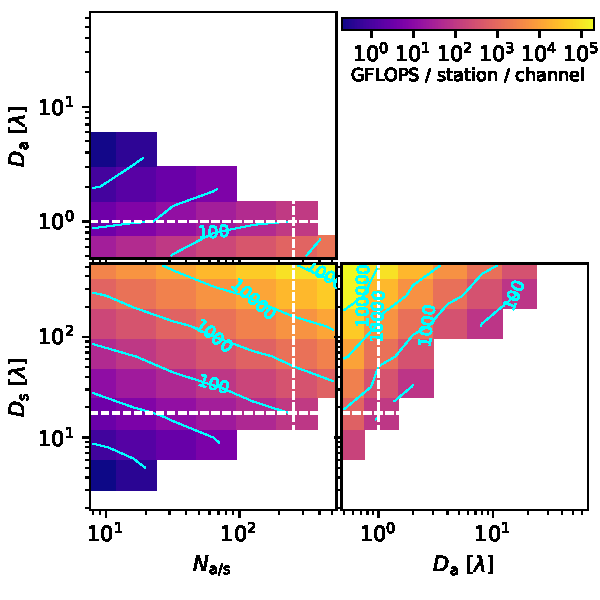
\includegraphics[width=0.4\textwidth]{figures/multidim_beamformer_dft_cost_analysis_SKA1-low.pdf}}
% \subfloat[][One-dimensional slices\label{fig:1D-incoherent-compcost-BF-SKA-low}]{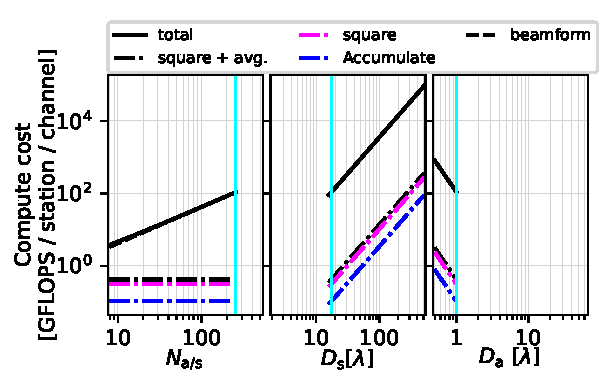
\includegraphics[width=0.58\textwidth]{figures/1D_beamformer_dft_cost_analysis_SKA1-low.pdf}}
% \caption{(Left): Two-dimensional slices of the computational cost for coherent-incoherent imaging using station-level voltage beamforming for \texttt{SKA-low-core}, \texttt{SKA-low}, \texttt{Aus-VLBA-low}, and \texttt{IC-VLBA-low}. Cyan contours  \label{fig:incoherent-compcost-BF-SKA-low}}
% \end{figure*}

Figure~\ref{fig:1D-incoherent-compcost-BF-LAMBDA-I} shows a breakdown of the computational cost per station per voxel for voltage beamforming as a function of the different station parameters. In each panel, all parameters except the one on the $x$-axis are kept fixed at the characteristic values of the \texttt{LAMBDA-I}, \textbf{\texttt{SKA-low}, and \texttt{SKA-low-core}} stations as highlighted in cyan. The total cost is dominated by the \textbf{DFT} beamforming in Equation~(\ref{eqn:intra-station-pol-hol-img-expl}) denoted by black dashed lines. \textbf{The DFT} beamforming cost per pixel scales linearly with the number of elements per station. The costs of squaring and temporal averaging in Equation~(\ref{eqn:intra-station-opt-pol-img-outprod}) are subdominant. Because the \textbf{squaring and temporal averaging} are performed on a per-pixel basis and not dependent on $N_\textrm{eps}$, they remain constant across $N_\textrm{eps}$. And because the number of independent pixels covering the field of view scales as $n_\textrm{bs} \simeq (D_\textrm{s}/D_\textrm{e})^2$, the cost per independent pixel remains constant across $D_\textrm{s}$ and $D_\textrm{e}$. All these operations have to be performed at every time step, $\delta t$, and hence remain constant regardless of $t_\textrm{acc}$. Although spatial averaging across multiple stations (orange dot-dashed line) is not a station-level operation, it is shown to emphasise that it constitutes only a negligible cost relative to the other components, noting that it needs to be only performed on a slower cadence of $t_\textrm{acc}$ on a per-pixel basis, and thus scales inversely with $t_\textrm{acc}$.

\begin{figure}
\includegraphics[width=\linewidth]
% {figures/1D_beamformer_dft_per_pixel_cost_analysis_LAMBDA-I.pdf}
{fig_02.pdf}
\caption{A breakdown of the computational cost density function over the station parameters for the voltage beamforming architecture at the station level. Each panel shows the variation with the respective parameter keeping the rest fixed at the characteristic values of the \textbf{\texttt{LAMBDA-I}, \texttt{SKA-low-core}, and \texttt{SKA-low} stations} (cyan lines). The beamforming cost in Equation~(\ref{eqn:intra-station-pol-hol-img-expl}) denoted by black dashed lines dominates the squaring (pink dot-dashes) and temporal averaging (blue dot-dashes) costs in Equation~(\ref{eqn:intra-station-opt-pol-img-outprod}). 
\label{fig:1D-incoherent-compcost-BF-LAMBDA-I}}
\end{figure}

Figure~\ref{fig:multidim-incoherent-compcost-BF-LAMBDA-I} shows a covariant view of the total computational cost density per station per voxel \textbf{(after summing the DFT, squaring, and averaging components)} for the beamforming architecture taken two station parameters at a time while keeping the rest fixed at the nominal values of a \texttt{LAMBDA-I}, \textbf{\texttt{SKA-low}, and a \texttt{SKA-low-core}} station (grey dashed lines). The variation in the cost per voxel is dominated by the beamforming cost and exhibits the same trends observed in Figure~\ref{fig:1D-incoherent-compcost-BF-LAMBDA-I}, that is, linear in $N_\textrm{eps}$ while remaining constant with $D_\textrm{e}$ and $D_\textrm{s}$. 

\begin{figure}
\includegraphics[width=\linewidth]
% {figures/multidim_beamformer_dft_per_pixel_cost_analysis_LAMBDA-I.pdf}
{fig_03.pdf}
\caption{A multi-dimensional covariant view of the net computational cost density function over the station parameters for the voltage beamforming architecture at the station level by varying two parameters at a time while fixing the rest at the nominal values of the \textbf{\texttt{LAMBDA-I}, \texttt{SKA-low-core}, and \texttt{SKA-low} stations} shown in grey dashed lines. The empty portions in the panels denote parts of parameter space physically impossible to sample given the constraints of the station parameters. Contours corresponding to the colour scale are shown in cyan. 
\label{fig:multidim-incoherent-compcost-BF-LAMBDA-I}}
\end{figure}

\subsection{E-field Parallel Imaging Correlator (EPIC)}

\textbf{Instead of DFT beamforming at discrete arbitrary locations as described above,} forming independent beams that simultaneously fill the entire field of view can be achieved by a two-dimensional spatial Fast Fourier Transform (FFT) of the \textbf{calibrated electric field} measurements on the aperture plane. \textbf{Typically, this has been associated with a regularly gridded array layout \citep{Daishido+1991,Otobe+1994,Tegmark+2009,Tegmark+2010,Foster+2014,Masui+2019}. However, it} can be enabled even for an irregular layout of station elements by gridding the calibrated electric fields measured by the station elements. The Optimal Map Making \citep[OMM;][]{Tegmark1997a} formalism adopted by \citet{Morales2011} is the basis of the architecture called E-field Parallel Imaging Correlator \cite[EPIC;][]{Thyagarajan+2017},
\begin{align}
    \widetilde{\mathcal{E}}_m^\alpha(\hat{\boldsymbol{s}}_k) &= \sum_j \delta^2 \boldsymbol{r}_j \, e^{i\frac{2\pi}{\lambda} \hat{\boldsymbol{s}}_k\cdot\boldsymbol{r}_j} \left(\sum_{a_m} \sum_p \widetilde{W}_{a_m}^{\alpha p*}(\boldsymbol{r}_j-\boldsymbol{r}_{a_m}) \, \widetilde{E}_{a_m}^p \right) \, . \label{eqn:intra-station-pol-hol-img-epic}
\end{align}
The expression within the parenthesis represents the gridding operation \textbf{of each calibrated electric field measurement at an arbitrary location, $\boldsymbol{r}_{a_m}$, of element $a_m$ onto a common grid at locations, $\boldsymbol{r}_j$, using a gridding kernel, $\widetilde{W}_{a_m}^{\alpha p*}(\boldsymbol{r}_j)$ corresponding to that element.} The outer summation denotes the Fourier transform \textbf{of the gridded electric fields} implemented via FFT. 

% whose equivalent linear algebraic representation is 
% \begin{align}
%   \widetilde{\boldsymbol{\mathcal{E}}}_{[m,\alpha,\hat{\boldsymbol{s}}]} &= \mathbf{F}^\textrm{H}_{[\hat{\boldsymbol{s}}\leftarrow \boldsymbol{r}]}\,\widetilde{\mathbf{W}}^\textrm{H}_{[\alpha,\boldsymbol{r}\leftarrow p,\boldsymbol{r}_{a_m}]}\,\widetilde{\mathbf{E}}_{[p,\boldsymbol{r}_{a_m}]} \, . \label{eqn:intra-station-pol-hol-img-epic-LA}
% \end{align}
% The subscripted variables on either side of $\leftarrow$ indicate the transformation carried out by the associated matrix. For example, $\mathbf{F}^\textrm{H}_{[\hat{\boldsymbol{s}}\leftarrow \boldsymbol{r}]}\coloneqq e^{i\frac{2\pi}{\lambda} \hat{\boldsymbol{s}}_k\cdot\boldsymbol{r}_j}$ denotes the Hermitian of the Fourier matrix (inverse Fourier matrix) transforming variables defined on aperture grid, $\boldsymbol{r}_j$, to sky grid, $\hat{\boldsymbol{s}}_k$. $\widetilde{\mathbf{W}}^\textrm{H}_{[\alpha,\boldsymbol{r}\leftarrow p,\boldsymbol{r}_{a_m}]}\coloneqq \{\widetilde{W}_{a}^{\alpha p *}(\boldsymbol{r}_j-\boldsymbol{r}_a)\}$ is a matrix, where each column corresponds to the gridding weights of an element, $\widetilde{W}_{a}^{\alpha p*}(\boldsymbol{r}_j)$, and the rows correspond to the aperture grid locations, $\boldsymbol{r}_j$. In each column, the gridding weights are shifted to the element location, $\boldsymbol{r}_{a}$. 
% % And, $\mathbf{W}_{[p,\boldsymbol{r}_{a}\leftarrow \alpha,\boldsymbol{r}]}\coloneqq \{W_{a}^{p\alpha}(\boldsymbol{r}_{a}-\boldsymbol{r}_j)\}$ is a matrix, where each row corresponds to the holographic pattern of an element, $W_{a}^{p\alpha}(\boldsymbol{r}_j)$, and the columns correspond to the aperture grid locations, $\boldsymbol{r}_j$. In each row, the holographic weights are shifted to the element location, $\boldsymbol{r}_{a}$. 

Application of the FFT will have the effect of simultaneously beamforming over the entire field of view, $\Omega_\textrm{e}$. The convolution with $\widetilde{W}_{a_m}^{\alpha p*}(\boldsymbol{r})$ in the aperture, which is the Fourier transform equivalent of $\widetilde{\mathcal{W}}_{a_m}^{{\alpha p}^*}(\hat{\boldsymbol{s}}_k)$, has several purposes. Firstly, it can be chosen to optimise specific properties in the synthesised image. For example, choosing $\widetilde{W}_{a_m}^{\alpha p*}(\boldsymbol{r})=W_{a_m}^{\alpha p*}(\boldsymbol{r})$, \textbf{the complex conjugate of} the holographic illumination pattern of the antenna element, $a_m$, will optimise the signal-to-noise ratio in the image \citep{Morales2011}. \textbf{Secondly, it can incorporate $w$-projection for non-coplanar element spacings \citep{Cornwell+2008}, direction-dependent ionospheric effects, wide-field distortions from refractive and scintillating atmospheric distortions, etc. \citep{Morales+2009,Morales2011}.} Finally, it also acts as gridding convolution transforming data from discrete and arbitrary locations onto a regular grid, thereby facilitating the application of a two-dimensional spatial FFT. Finally, the polarised intensities are obtained by application of Equation~(\ref{eqn:intra-station-opt-pol-img-outprod}), \textbf{that is pixelwise ``squaring'' (outer product of polarisation states) and temporal averaging.}

% The polarised intensity on $\mathbb{S}$ is again given by Equation~(\ref{eqn:intra-station-opt-pol-img-outprod}), which is expressed linear algebraically as
% \begin{align}
%     \widetilde{\mathbf{I}}_{[m,\alpha\beta,\hat{\boldsymbol{s}}]} &= \left\langle \widetilde{\boldsymbol{\mathcal{E}}}_{[m,\alpha,\hat{\boldsymbol{s}}]} \bigotimes_{\alpha\beta} \widetilde{\boldsymbol{\mathcal{E}}}_{[m,\beta,\hat{\boldsymbol{s}}]}^* \right\rangle \, , \label{eqn:intra-station-opt-polarimetric-direct-img-LA}    
% \end{align}
% where, the outer product is performed over polarisation indices, $\alpha$ and $\beta$. 

Figure~\ref{fig:1D-incoherent-compcost-EPIC-LAMBDA-I} shows a breakdown of the costs per station per voxel of the EPIC architecture, with nominal values of a \texttt{LAMBDA-I}, \textbf{\texttt{SKA-low}, or a \texttt{SKA-low-core}} station marked in cyan. The dominant cost is from the two-dimensional FFT (black dashed lines) in Equation~\ref{eqn:intra-station-pol-hol-img-epic}.
% or equivalently, Equation~\ref{eqn:intra-station-pol-hol-img-epic-LA}.
The spatial FFT cost depends only on the grid dimensions. So, it is independent of $N_\textrm{eps}$ as the grid can hold \textbf{as many} $N_\textrm{eps}$ elements as physically possible. The \textbf{computational cost of the} spatial FFT scales roughly as $(\gamma_\textrm{s} \, D_\textrm{s}/D_\textrm{e})^2\log_2(\gamma_\textrm{s}\, D_\textrm{s}/D_\textrm{e})^2$, where, $\gamma_\textrm{s}$ is a constant padding factor. \textbf{$\gamma_\textrm{s}$ is used to control the pixel scale in the image. For example, $\gamma_\textrm{s}=2$ (adopted in this paper) will provide identical pixel scale and image size as that formed from gridded visibilities.} Notably, because the spatial FFT produces an image over the entire field of view at every independent pixel instantly, it is not a pixelwise operation, and therefore, its cost per pixel scales as $\sim \log_2(D_\textrm{s}/D_\textrm{e})$, which exhibits a weak dependence on $D_\textrm{s}$ and $D_\textrm{e}$. The squaring (pink dot-dashed lines) and temporal averaging (blue dot-dashed lines) \textbf{in Equation~\ref{eqn:intra-station-opt-pol-img-outprod} operate on a per-pixel basis. Thus, those} costs per voxel remain constant with $N_\textrm{eps}$, $D_\textrm{s}$ and $D_\textrm{e}$ similar to the voltage beamforming architecture. And they 
% {eqn:intra-station-opt-polarimetric-direct-img-LA}
are subdominant. The gridding (black dotted lines) with weights in Equation~(\ref{eqn:intra-station-pol-hol-img-epic})
% and (\ref{eqn:intra-station-pol-hol-img-epic-LA})
is a per-element operation and depends only on $N_\textrm{eps}$ \textbf{and the size of the gridding kernel, $N_\textrm{ke}$. Here, $N_\textrm{ke}=1$ is chosen to provide unaliased full field-of-view images. The incorporation of $w$-projection in the gridding kernel will correspondingly increase $N_\textrm{ke}$. Nevertheless, the gridding cost}, scales linearly with $N_\textrm{eps}$ and inverse squared with $D_\textrm{s}$ per voxel. Overall, the gridding cost is insignificant. Again, the spatial averaging of pixels across multiple stations (orange dot-dashed line) is not a station-level operation, but is only shown to emphasise that it operates on a much slower cadence of $t_\textrm{acc}$, scaling inversely with $t_\textrm{acc}$, and adds only negligible cost to the overall cost budget. 

\begin{figure}
\includegraphics[width=0.99\linewidth]
% {figures/1D_epic_per_pixel_cost_analysis_LAMBDA-I.pdf}
{fig_04.pdf}
\caption{A breakdown of the computational cost density function over the station parameters for the EPIC architecture at the station level. Each panel shows the variation with the respective parameter keeping the rest fixed at the characteristic values of the \textbf{\texttt{LAMBDA-I}, \texttt{SKA-low-core}, and \texttt{SKA-low} stations} (cyan lines). The spatial FFT cost in Equation~(\ref{eqn:intra-station-pol-hol-img-epic})
  % {eqn:intra-station-pol-hol-img-epic-LA}
  denoted by black dashed lines dominates the squaring (pink dot-dashes) and temporal averaging (blue dot-dashes) costs in Equation~(\ref{eqn:intra-station-opt-pol-img-outprod}).
  % {eqn:intra-station-opt-polarimetric-direct-img-LA}
  The gridding operation (black dotted lines) in Equation~(\ref{eqn:intra-station-pol-hol-img-epic})
  % {eqn:intra-station-pol-hol-img-epic-LA}
  contributes even lesser to the cost budget. 
\label{fig:1D-incoherent-compcost-EPIC-LAMBDA-I}}
\end{figure}

Figure~\ref{fig:multidim-incoherent-compcost-EPIC-LAMBDA-I} shows a covariant view of the total computational cost density per station per voxel \textbf{(sum of gridding, FFT, squaring and temporal averaging components)} for the EPIC architecture taken two station parameters at a time while keeping the rest fixed at the nominal values of a \texttt{LAMBDA-I}, \textbf{\texttt{SKA-low}, or a \texttt{SKA-low-core}} station denoted by grey dashed lines. The variation in the cost per voxel is dominated by the spatial FFT cost which is relatively constant in all these parameters and displays the same trends observed in Figure~\ref{fig:1D-incoherent-compcost-EPIC-LAMBDA-I}, namely, nearly constant in $N_\textrm{eps}$, $D_\textrm{e}$ and $D_\textrm{s}$. Figure~\ref{fig:multidim-incoherent-relative-compcost-EPIC-LAMBDA-I} shows the ratio of the computational cost of the EPIC architecture relative to the voltage beamforming architecture in Figure~\ref{fig:multidim-incoherent-compcost-BF-LAMBDA-I}. It is clearly noted that the cost of the EPIC architecture is significantly less than that of voltage beamforming for $N_\textrm{eps} \gtrsim 100$, and continues to decrease with increasing $N_\textrm{eps}$, implying that for full field of view imaging, EPIC has a clear and significant computational advantage over voltage \textbf{DFT} beamforming as $N_\textrm{eps}$ and packing density of elements in a station increase.

\begin{figure*}
\centering
\subfloat[][Covariant cost density of EPIC architecture \label{fig:multidim-incoherent-compcost-EPIC-LAMBDA-I}]{\includegraphics[width=0.48\textwidth]
% {figures/multidim_epic_per_pixel_cost_analysis_LAMBDA-I.pdf}
{fig_05a.pdf}  
}
\subfloat[][Covariant cost of EPIC architecture relative to BF architecture \label{fig:multidim-incoherent-relative-compcost-EPIC-LAMBDA-I}]{\includegraphics[width=0.48\textwidth]
% {figures/multidim_epic_relative_cost_analysis_LAMBDA-I.pdf}
{fig_05b.pdf}
} 
\caption{(Left): Two-dimensional slices of the computational cost per station per voxel for coherent-incoherent imaging using station-level EPIC. Because the spatial FFT dominates the overall cost budget, the computational cost density is relatively insensitive to $N_\textrm{eps}$, $D_\textrm{s}$, and $D_\textrm{e}$ \textbf{as seen in Figure~\ref{fig:1D-incoherent-compcost-EPIC-LAMBDA-I}, thereby not showing much variation in the colour scale.} (Right): Ratio of computational cost of EPIC to voltage beamforming. For $N_\textrm{eps}\gtrsim 100$, EPIC has a significant advantage over voltage beamforming. Gray dashed lines indicate nominal values for \textbf{\texttt{LAMBDA-I}, \texttt{SKA-low-core}, and \texttt{SKA-low} stations}. Logarithmic contour levels corresponding to the colour scale are shown in cyan. \label{fig:incoherent-compcost-EPIC-LAMBDA-I}}
\end{figure*}

\textbf{The EPIC architecture has been implemented on the Long Wavelength Array (LWA) station in Sevilleta (NM, USA) \cite{Kent+2019,Kent+2020,Krishnan+2023} using a GPU framework and operates on a commensal mode. With recent optimisations, the EPIC pipeline on LWA-Sevilleta computes $128\times 128$ all-sky images at 25,000 frames per second and outputs at a cadence of 40--80~ms accumulations \citep{Reddy+2024}. For reference, the software correlator and visibility-based imager can produce images at 5~s cadence \citep{Taylor+2012}.}

\textbf{The EPIC architecture will be relevant for large cosmological arrays like PUMA that are considering a FFT-based correlator architecture. Obtaining visibilities from an EPIC architecture will involve an additional step of an inverse-FFT or an inverse-DFT back to the aperture plane from the accumulated images (not included in Figure~\ref{fig:1D-incoherent-compcost-EPIC-LAMBDA-I}). However, the inverse-FFT or DFT operation to obtain visibilities needs to be performed only once every accumulation interval, and is thus not expected to add significantly to the total cost budget.} 

\subsection{Correlator Beamforming (XBF)}

\textbf{In the traditional correlator approach, a pair of electric field measurements, $E_{a_m}^p$ and $E_{b_m}^q$, in polarisation states, $p$ and $q$, at station elements, $a_m$ and $b_m$, respectively, can be cross-correlated and temporally averaged to obtain} calibrated visibilities, $\widetilde{V}_{a_m b_m}^{pq}$, in a station, $m$. It can be written as 
\begin{align}
    \widetilde{V}_{a_m b_m}^{pq} &= \bigl\langle E_{a_m}^p \, E_{b_m}^{q*}\bigr\rangle \, . \label{eqn:intra-station-pol-visibilities}
\end{align}
\textbf{The visibilities in the station} can be beamformed using a DFT to obtain polarised intensities in any desired direction, $\boldsymbol{s}_k$, as
\begin{align}
    \widetilde{\mathcal{I}}_m^{\alpha\beta}(\hat{\boldsymbol{s}}_k) 
    &= \sum_{a_m,b_m} \sum_{p,q} \widetilde{\mathcal{B}}_{a_m b_m}^{\alpha\beta;pq*}(\hat{\boldsymbol{s}}_k) \, \widetilde{V}_{a_m b_m}^{pq} \,  e^{i\frac{2\pi}{\lambda} \hat{\boldsymbol{s}}_k\cdot\Delta\boldsymbol{r}_{a_m b_m}} \, . \label{eqn:intra-station-pol-xbf-img-expl} 
\end{align}
$\widetilde{\mathcal{B}}_{a_m b_m}^{\alpha\beta;pq*}(\hat{\boldsymbol{s}}_k)$, is the counterpart of $\widetilde{\mathcal{W}}_{a_m}^{{p\alpha}^*}(\hat{\boldsymbol{s}}_k)$ in Equation~(\ref{eqn:intra-station-pol-hol-img-expl}) for a correlated quantity, and it denotes a complex-valued directional weighting applied to the calibrated visibility \textbf{representing the contribution of polarisation state, $pq$, to a state, $\alpha\beta$, in the measurement and sky planes, respectively.} It can be chosen to produce images with desired characteristics \citep{Masui+2019}. 
% This correlation beamforming step can be executed at a cadence of $t_\textrm{acc}$. However, the correlations that produce visibilities must still be executed on timescales of $\delta t$. Like voltage beamforming, the number of independent beams filling the field of view is $n_\textrm{bs} \simeq (D_\textrm{s}/D_\textrm{e})^2$. 

Figure~\ref{fig:1D-incoherent-compcost-XBF-LAMBDA-I} shows the computational cost density breakdown for correlator beamforming at the station level. The correlation and temporal averaging in Equation~(\ref{eqn:intra-station-pol-visibilities}) \textbf{are performed on every pair of station elements and} scale as $N_\textrm{eps}(N_\textrm{eps}-1)/2$, with no dependence on $D_\textrm{e}$ or $D_\textrm{s}$. Hence, their per pixel costs scale as $(D_\textrm{s}/D_\textrm{e})^{-2}$. The two-dimensional DFT in Equation~(\ref{eqn:intra-station-pol-xbf-img-expl}) also scales as $N_\textrm{eps}(N_\textrm{eps}-1)/2$, but being a per-pixel operation, stays constant with $D_\textrm{e}$ and $D_\textrm{s}$. The correlation and temporal averaging have to be performed at every interval of $\delta t$ and are therefore, independent of $t_\textrm{acc}$, whereas the DFT needs to be performed at a cadence of $t_\textrm{acc}$ and thus scales as $t_\textrm{acc}^{-1}$. For the chosen parameters of \texttt{LAMBDA-I}, \textbf{\texttt{SKA-low}, and \texttt{SKA-low-core},} at $t_\textrm{acc}=1$~ms, the computational cost density is dominated by the cost of the DFT. However, for imaging on a slower cadence, $t_\textrm{acc}\gtrsim 10$~ms, the cost of correlation begins to dominate. 

% The computational cost budget consists of the following components. The formation of polarimetric visibilities and their accumulations requires $n_\textrm{p}^2 N_\textrm{eps} (N_\textrm{eps}-1)/2$ complex multiplications and complex additions, respectively, per station per channel at a cadence of $\delta t$. These accumulated visibilities will be further averaged across stations but on a slower cadence of $t_\textrm{acc}$. However, in order to obtain stationwise image intensities, we will not consider averaging across stations. Thus, the computational cost of forming polarimetric visibilities and their accumulations per station per channel is $4 n_\textrm{p}^2 N_\textrm{eps} (N_\textrm{eps}-1)/(\delta t)$ FLOPS. The accumulated visibilities from a station can be beamformed towards $n_\textrm{bs}\simeq (D_\textrm{s}/D_\textrm{e})^2$ sky locations using a DFT to obtain Stokes intensities. This DFT beamforming performs $n_\textrm{p}^2 N_\textrm{eps} (N_\textrm{eps}-1) (D_\textrm{s}/D_\textrm{e})^2 /2$ CMACs at a slower cadence of $t_\textrm{acc}$. Hence, the net computational cost for DFT beamforming of visibilities across the field of view per station per channel is 
% \begin{align}
%     C_\textrm{XBF} &= 4 n_\textrm{p}^2 \, N_\textrm{eps} (N_\textrm{eps}-1) \left[\frac{1}{\delta t} + \frac{\left(D_\textrm{s}/D_\textrm{e}\right)^2}{t_\textrm{acc}} \right] \, . \label{eqn:cost-XBF}
% \end{align}

\begin{figure}
\includegraphics[width=\linewidth]
% {figures/1D_xcor_dft_per_pixel_cost_analysis_LAMBDA-I.pdf}
{fig_06.pdf}
\caption{A breakdown of the computational cost density function over the station parameters for the correlator beamforming architecture (XBF) at the station level. Each panel shows the variation with the respective parameter keeping the rest fixed at the characteristic values of the \texttt{LAMBDA-I}, \texttt{SKA-low-core}, and \texttt{SKA-low} stations (cyan lines). The two-dimensional DFT (dashed lines) dominates the cost for the chosen \texttt{LAMBDA-I} parameters at an imaging cadence of $t_\textrm{acc}=1$~ms over correlation (double dot-dashed) and temporal averaging of the correlations (dot-dashed).
% The spatial FFT cost in Equation~(\ref{eqn:intra-station-pol-hol-img-epic-LA}) denoted by black dashed lines dominates the squaring (pink dot-dashes) and temporal averaging (blue dot-dashes) costs in Equation~(\ref{eqn:intra-station-opt-polarimetric-direct-img-LA}). The gridding operation (black dotted lines) in Equation~(\ref{eqn:intra-station-pol-hol-img-epic-LA}) contributes even lesser to the cost budget. 
\label{fig:1D-incoherent-compcost-XBF-LAMBDA-I}}
\end{figure}

Figure~\ref{fig:multidim-incoherent-compcost-XBF-LAMBDA-I} is a covariant view of the total computational cost density per station per voxel \textbf{(sum of correlator, temporal averaging, and DFT components)} for the correlator beamformer architecture taken two station parameters at a time while keeping the rest fixed at the nominal values of a \texttt{LAMBDA-I} station (grey dashed lines). The variation in the cost per voxel for $t_\textrm{acc}=1$~ms is dominated by the spatial DFT cost which is relatively constant in $D_\textrm{e}$ and $D_\textrm{s}$, and scales as $\sim N_\textrm{eps}^2$, displaying the same trends observed in Figure~\ref{fig:1D-incoherent-compcost-XBF-LAMBDA-I}. Figure~\ref{fig:multidim-incoherent-relative-compcost-XBF-LAMBDA-I} shows the ratio of the computational cost of the XBF architecture relative to the voltage beamforming architecture in Figure~\ref{fig:multidim-incoherent-compcost-BF-LAMBDA-I}. It is clear that the cost of the XBF architecture is less expensive only for $N_\textrm{eps}\lesssim 100$, and gets worse with increasing $N_\textrm{eps}$.

\begin{figure*}
\centering
\subfloat[][Covariant cost density of XBF architecture \label{fig:multidim-incoherent-compcost-XBF-LAMBDA-I}]
{\includegraphics[width=0.48\textwidth]
% {figures/multidim_xcor_dft_per_pixel_cost_analysis_LAMBDA-I.pdf}
{fig_07a.pdf}
}
\subfloat[][Covariant cost of XBF architecture relative to BF architecture \label{fig:multidim-incoherent-relative-compcost-XBF-LAMBDA-I}]
{\includegraphics[width=0.48\textwidth]
% {figures/multidim_xcor_dft_relative_cost_analysis_LAMBDA-I.pdf}
{fig_07b.pdf}
}
\caption{(Left): Two-dimensional slices of the computational cost for coherent-incoherent imaging using a DFT of station-level cross-correlations for \texttt{LAMBDA-I}, \texttt{SKA-low-core}, and \texttt{SKA-low} station parameters (dashed gray lines). Cyan lines denote contours of the colour scale in logarithmic increments. (Right): Same as the left but relative to a voltage beamformer architecture. The computational cost density is dominated by the two-dimensional DFT cost for $t_\textrm{acc}=1$~ms, and is lower than that of voltage beamforming for $N_\textrm{eps}\lesssim 100$ while getting more expensive with increasing $N_\textrm{eps}$. \label{fig:incoherent-compcost-XBF-LAMBDA-I}}
\end{figure*}

\subsection{Correlation and FFT (XFFT)}

In this approach, $\widetilde{V}_{a_m b_m}^{pq}$, the calibrated and inverse noise covariance weighted visibilities in station, $m$, in Equation~(\ref{eqn:intra-station-pol-visibilities}) are gridded with weights, $\widetilde{B}_{a_m b_m}^{\alpha\beta;pq*}(\Delta\boldsymbol{r}_j-\Delta\boldsymbol{r}_{a_m b_m})$, the Fourier transform equivalent of $\widetilde{\mathcal{B}}_{a_m b_m}^{\alpha\beta;pq*}(\hat{\boldsymbol{s}}_k)$ in Equation~(\ref{eqn:intra-station-pol-xbf-img-expl}), onto a grid and Fourier transformed using an FFT rather than the discrete Fourier transform of correlator beamforming,
\begin{align}
  \widetilde{\mathcal{I}}_m^{\alpha\beta}(\hat{\boldsymbol{s}}_k) &= \sum_j \delta^2 \Delta\boldsymbol{r}_j \, e^{i\frac{2\pi}{\lambda} \hat{\boldsymbol{s}}_k\cdot\Delta\boldsymbol{r}_j} \nonumber\\
  &\quad \left(\sum_{a_m,b_m} \sum_p \widetilde{B}_{a_m b_m}^{\alpha\beta;pq*}(\Delta\boldsymbol{r}_j-\Delta\boldsymbol{r}_{a_m b_m}) \, \widetilde{V}_{a_m b_m}^{pq} \right) \, . \label{eqn:intra-station-pol-img-xfft-expl}
\end{align}
The gridding and Fourier transform (using FFT) are represented by the parenthesis and outer summation, respectively. 

This is the mathematical counterpart to the operations performed on calibrated electric fields from the elements in EPIC, with few key differences -- (1) the calibrated visibilities can be accumulated and allowed for Earth rotation and bandwidth synthesis, (2) the gridding and spatial Fourier transform operate not on electric fields but visibilities, and (3) the spatial Fourier transform can occur on a slower cadence of $t_\textrm{acc}$.
% This is an explicit form of the optimal map-making (OMM) formalism \citep{Tegmark1997a}, and provides a lossless and optimal (least-squares) solution, which
In the radio interferometric context, $\widetilde{\mathcal{I}}_m^{\alpha\beta}(\hat{\boldsymbol{s}}_k)$ is referred to as the ``dirty image'' \citep{TMS2017,SIRA-II}. The purpose of $\widetilde{B}_{a_m b_m}^{\alpha\beta;pq*}(\Delta\boldsymbol{r}_j-\Delta\boldsymbol{r}_{a_m b_m})$ is similar \citep{Morales+2009,Bhatnagar+2008,Cornwell+2008} to its counterpart gridding operator in the EPIC architecture \citep{Morales2011}. 

% The optimal map-making (OMM) formalism \citep{Tegmark1997a} provides a lossless and optimal (least-squares) solution, which in the radio interferometric context is often referred to as the ``dirty image'' \citep{TMS2017,SIRA-II}, and can be expressed linear algebraically as \citep{Bhatnagar+2008,Morales+2009}:
% \begin{align}
%     \widetilde{\mathbf{I}}_{[m,\alpha\beta,\hat{\boldsymbol{s}}]} &=  \mathbf{F}^\textrm{H}_{[\hat{\boldsymbol{s}}\leftarrow\Delta\boldsymbol{r}]}\,\widetilde{\mathbf{B}}^\textrm{H}_{[\alpha\beta,\Delta\boldsymbol{r}\leftarrow pq,\Delta\boldsymbol{r}_{a_m b_m}]} \nonumber\\ 
%     &\qquad \mathbf{N}^{-1}_{[\Delta\boldsymbol{r}_{a_m b_m}\leftarrow\Delta\boldsymbol{r}_{a_m b_m}]}\,\widehat{\mathbf{V}}_{[pq,\Delta\boldsymbol{r}_{a_m b_m}]} \label{eqn:intra-station-opt-pol-corr-image}
%     % &= \mathbf{F}^\textrm{H}_{[\hat{\boldsymbol{s}}\leftarrow\Delta\boldsymbol{r}]}\,\mathbf{B}^\textrm{H}_{[\Delta\boldsymbol{r}\leftarrow\Delta\boldsymbol{r}_{a_m b_m}]}\,\mathbf{N}^{-1}_{[\Delta\boldsymbol{r}_{a_m b_m}\leftarrow\Delta\boldsymbol{r}_{a_m b_m}]} \nonumber\\ 
%     % &\qquad\qquad\qquad \vect\left(\Bigl\langle\widehat{\mathbf{E}}_{[\boldsymbol{r}_{a_m}]}\widehat{\mathbf{E}}^\textrm{H}_{[\boldsymbol{r}_{b_m}]}\Bigl\rangle\right)_{[\Delta\boldsymbol{r}_{a_m b_m}]} \, . \label{eqn:opt-copolar-corr-image}
% \end{align}
% % The subscript, $m$, on the left hand side denotes that the image was made using measurements within the station, $m$. 
% The inversion operation above takes a column vector of calibrated visibilities, $\widehat{\mathbf{V}}_{[pq,\Delta\boldsymbol{r}_{a_m b_m}]}\coloneqq \vect\left(\Bigl\langle\widehat{\mathbf{E}}_{[p,\boldsymbol{r}_{a_m}]}\widehat{\mathbf{E}}^\textrm{H}_{[q,\boldsymbol{r}_{b_m}]}\Bigl\rangle\right)$ at element spacings, $\Delta\boldsymbol{r}_{a_m b_m}$, in station $m$, weights them by the inverse noise covariance, $\mathbf{N}_{[\Delta\boldsymbol{r}_{a_m b_m}\leftarrow\Delta\boldsymbol{r}_{a_m b_m}]}\coloneqq \langle \boldsymbol{n}_{[\Delta\boldsymbol{r}_{a_m b_m}]}\boldsymbol{n}^\textrm{H}_{[\Delta\boldsymbol{r}_{a_m b_m}]}\rangle$, then weights and projects this inverse noise-covariance weighted vector of visibilities onto a finely sampled grid denoted by $\Delta\boldsymbol{r}$ using the gridding operator $\widetilde{\mathbf{B}}^\textrm{H}_{[\alpha\beta,\Delta\boldsymbol{r}\leftarrow pq,\Delta\boldsymbol{r}_{a_m b_m}]}$, and inverse-Fourier transforms using $\mathbf{F}^\textrm{H}_{[\hat{\boldsymbol{s}}\leftarrow\Delta\boldsymbol{r}]}$ to obtain for station, $m$, the estimate of the vector of pixelized intensities, $\widetilde{\mathbf{I}}_{[m,\alpha\beta,\hat{\boldsymbol{s}}]}$, on $\mathbb{S}$. 

% \begin{align}
%     \widetilde{\mathcal{I}}_m^{\alpha\beta}(\hat{\boldsymbol{s}}_k) 
%     &= \sum_{a_m,b_m} \sum_{p,q} \widetilde{\mathcal{B}}_{a_m b_m}^{*pq;\alpha\beta}(\hat{\boldsymbol{s}}_k) \, \widetilde{V}_{a_m b_m}^{pq} \,  e^{i\frac{2\pi}{\lambda} \hat{\boldsymbol{s}}_k\cdot\Delta\boldsymbol{r}_{a_m b_m}} \, , \label{eqn:intra-station-pol-xfft-img-expl} 
% \end{align}



% The purpose of $\widetilde{\mathbf{B}}^\textrm{H}_{[\alpha\beta,\Delta\boldsymbol{r}\leftarrow pq,\Delta\boldsymbol{r}_{a_m b_m}]}$ is similar \citep{Morales+2009,Cornwell+2008} to its counterpart gridding operator in the EPIC architecture \citep{Morales2011}. 
% % implies the following. First, if $\widetilde{\mathbf{B}}^\textrm{H}=\mathbf{B}^\textrm{H}$ (assumed hereafter, unless specified), then the inversion is lossless and optimal, minimizing noise and the reconstruction error \citep{Tegmark1997a}. This form is very similar to a matched filter. Second, it transforms the inverse noise covariance weighted visibilities at arbitrary locations, $\Delta\boldsymbol{r}_{a_m b_m}$, to finely sampled locations, $\Delta\boldsymbol{r}$, on a grid. If the grid is uniformly sampled, it facilitates efficient inverse Fourier transform using Fast Fourier Transform (FFT) algorithms. 
% Noting that the optimal inversion is weighted by $\widetilde{\mathbf{B}}^\textrm{H}$, which is the conjugate of that in the RIME in Equation~(\ref{eqn:RIME-LA}), the phase introduced by the instrument is cancelled out precisely during the inversion. However, the amplitude is not. Hence, the inverted image, $\widetilde{\mathbf{I}}_{[\hat{\boldsymbol{s}}]}$, is attenuated relative to the true image, $\mathbf{I}_{[m,\alpha\beta,\hat{\boldsymbol{s}}]}$, by a factor that is square of the interferometer's angular power pattern \citep{Cornwell+2008,Morales+2009}, once due to $\mathbf{B}_{[pq,\Delta\boldsymbol{r}_{a_m b_m}\leftarrow \alpha\beta,\Delta\boldsymbol{r}]}$ in Equation~(\ref{eqn:RIME-LA}) (inherent in the measurement) and once more due to $\widetilde{\mathbf{B}}^\textrm{H}_{[\alpha\beta,\Delta\boldsymbol{r}\leftarrow pq,\Delta\boldsymbol{r}_{a_m b_m}]}$ in Equation~(\ref{eqn:intra-station-opt-pol-corr-image}). 

% The computational cost consists of forming the visibilities and accumulating them, gridding them using the gridding kernel and accumulating them on the grid in case of overlapping data, and spatial FFT to obtain the polarimetric images. 

% \begin{table*}[htb!]
% \normalsize
% \begin{threeparttable}
% \caption{Computational budget of intra-station coherent imaging architectures}
% \label{tab:intra-station-coherent-imaging}
% \begin{tabular}{ccccc}
% % \begin{tabularx}{\textwidth}{ccccc}
% \toprule
% \headrow Intra-station & Components & Equation & FLOP count & Timescale \\
% architecture & & & (per station per channel) & \\ 
% \midrule\midrule
% BF & Beamforming & \ref{eqn:intra-station-pol-hol-img-expl} & $8 n_\textrm{p}^2 N_\textrm{eps} \left(\frac{D_\textrm{s}}{D_\textrm{e}}\right)^2$ & $\delta t$ \\
% & Squaring & \ref{eqn:intra-station-opt-pol-img-outprod} & $6 n_\textrm{p}^2 \left(\frac{D_\textrm{s}}{D_\textrm{e}}\right)^2$ & $\delta t$ \\
% & Accumulation & \ref{eqn:intra-station-opt-pol-img-outprod} & $2 n_\textrm{p}^2 \left(\frac{D_\textrm{s}}{D_\textrm{e}}\right)^2$ & $\delta t$ \\
% \midrule
% EPIC & Gridding & \ref{eqn:intra-station-pol-hol-img-epic-LA} & $6 n_\textrm{p}^2 N_\textrm{eps} N_\textrm{ke}$ & $\delta t$ \\
% & FFT & \ref{eqn:intra-station-pol-hol-img-epic-LA} & $8 n_\textrm{p} \frac{r}{\log_2 r} \left(\gamma_\textrm{s}\frac{D_\textrm{s}}{D_\textrm{e}}\right)^2\log_2\left(\gamma_\textrm{s}\frac{D_\textrm{s}}{D_\textrm{e}}\right)^2$ & $\delta t$ \\
% & Squaring & \ref{eqn:intra-station-opt-polarimetric-direct-img-LA} & $6 n_\textrm{p}^2 \left(\gamma_\textrm{s} \frac{D_\textrm{s}}{D_\textrm{e}}\right)^2$ & $\delta t$ \\
% & Accumulation & \ref{eqn:intra-station-opt-polarimetric-direct-img-LA} & $2 n_\textrm{p}^2 \left(\gamma_\textrm{s} \frac{D_\textrm{s}}{D_\textrm{e}}\right)^2$ & $\delta t$ \\
% \midrule
% XBF & Correlator & \ref{eqn:intra-station-pol-visibilities} & $6 n_\textrm{p}^2 N_\textrm{eps} (N_\textrm{eps}-1)/2$ & $\delta t$ \\
% & Accumulation & \ref{eqn:intra-station-pol-visibilities} & $2 n_\textrm{p}^2 N_\textrm{eps} (N_\textrm{eps}-1)/2$ & $\delta t$ \\
% & DFT & \ref{eqn:intra-station-pol-xbf-img-expl} & $8 n_\textrm{p}^2 \left(\frac{D_\textrm{s}}{D_\textrm{e}}\right)^2 N_\textrm{eps} (N_\textrm{eps}-1)/2$ & $t_\textrm{acc}$ \\
% \midrule
% XFFT & Correlator & \ref{eqn:intra-station-pol-visibilities} & $6 n_\textrm{p}^2 N_\textrm{eps} (N_\textrm{eps}-1)/2$ & $\delta t$ \\
% & Accumulation & \ref{eqn:intra-station-pol-visibilities} & $2 n_\textrm{p}^2 N_\textrm{eps} (N_\textrm{eps}-1)/2$ & $\delta t$ \\
% & Gridding & \ref{eqn:intra-station-opt-pol-corr-image} & 8$n_\textrm{p}^4 (2^2 N_\textrm{ke}) N_\textrm{eps} (N_\textrm{eps}-1)/2$ & $t_\textrm{acc}$ \\
% & FFT & \ref{eqn:intra-station-opt-pol-corr-image} & $8 n_\textrm{p}^2 \frac{r}{\log_2 r} \left(\frac{D_\textrm{s}}{D_\textrm{e}}\right)^2\log_2\left(\frac{D_\textrm{s}}{D_\textrm{e}}\right)^2$ & $t_\textrm{acc}$ \\
% % \midrule
% % Three & Four&three three\tnote{b} &four & & \\
% \bottomrule
% % \end{tabularx}
% \end{tabular}
% \begin{tablenotes}[hang]
% % \item[]Table note
% \item[a]Array filling factor, $\,f_\textrm{A}=N_\textrm{s}\,(D_\textrm{s}/D_\textrm{A})^2$
% % \item[b]Station filling factor, $\,f_\textrm{s}=N_\textrm{eps}\,(D_\textrm{e}/D_\textrm{s})^2$
% \end{tablenotes}
% \end{threeparttable}
% \end{table*}

% \subsubsection{Correlator Beamforming (XBF)}

% \begin{figure*}
% \centering
% \subfloat[][Two-dimensional slices \label{fig:multidim-incoherent-compcost-XBF-SKA-low}]{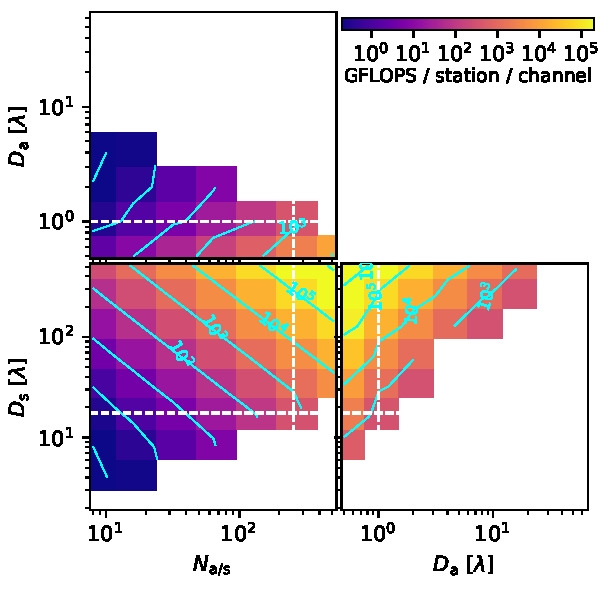
\includegraphics[width=0.48\textwidth]{figures/multidim_xcor_dft_cost_analysis_SKA1-low.pdf}}
% \subfloat[][Two-dimensional slices (relative)\label{fig:multidim-incoherent-relative-compcost-XBF-SKA-low}]{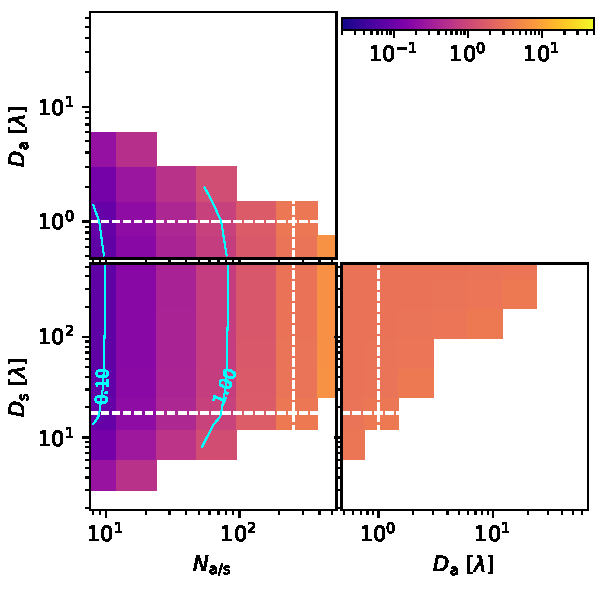
\includegraphics[width=0.48\textwidth]{figures/multidim_xcor_dft_relative_cost_analysis_SKA1-low.pdf}}
% \caption{(Left): Two-dimensional slices of the computational cost for coherent-incoherent imaging using a DFT of station-level cross-correlations for \texttt{SKA-low-core}, \texttt{SKA-low}, \texttt{Aus-VLBA-low}, and \texttt{IC-VLBA-low}. Cyan contours  \label{fig:incoherent-compcost-XBF-SKA-low}}
% \end{figure*}

% \begin{figure}
% 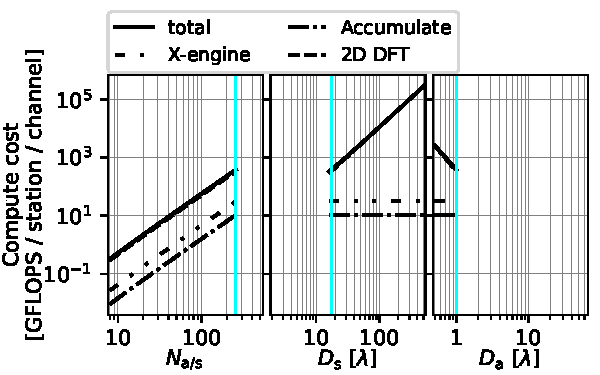
\includegraphics[width=\linewidth]{figures/1D_xcor_dft_cost_analysis_SKA1-low.pdf}
% % 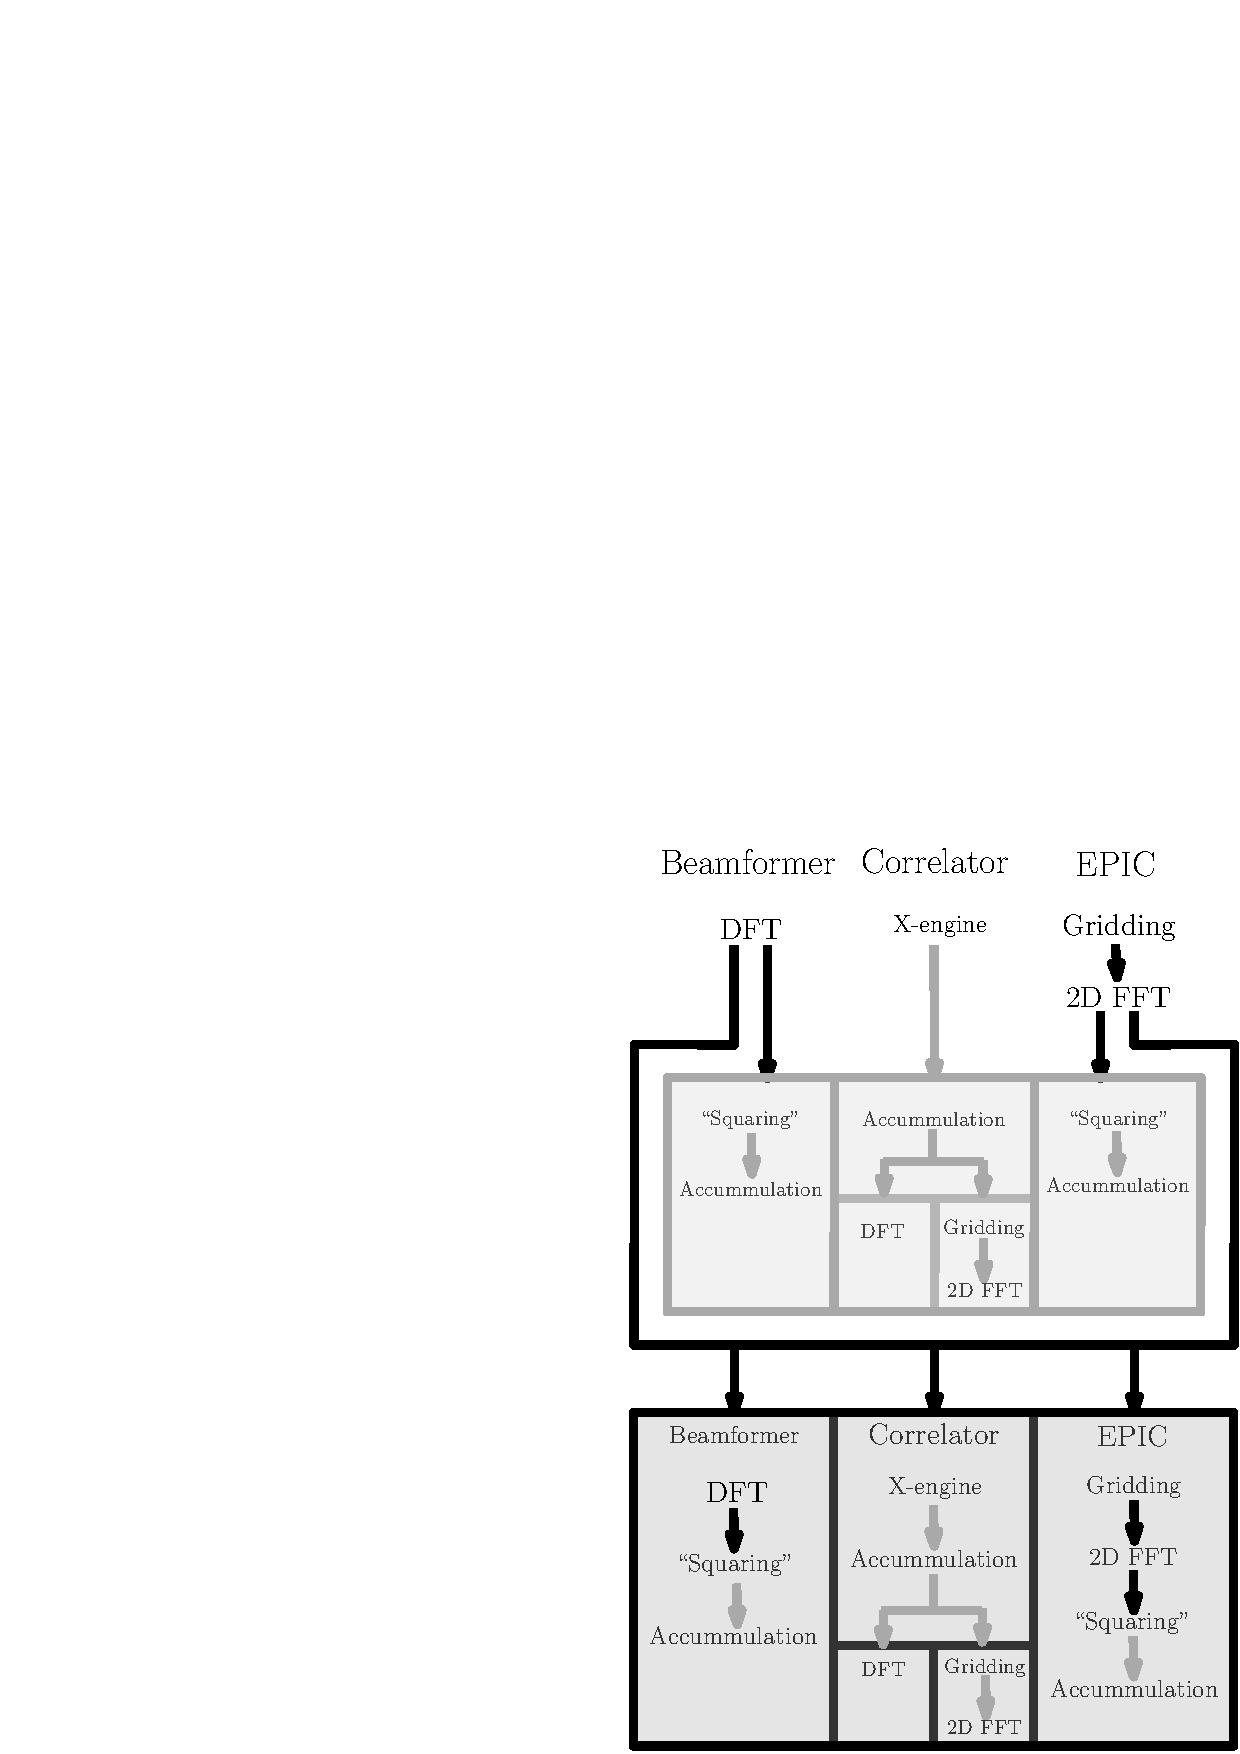
\includegraphics[width=\linewidth]{fig_01.pdf}
% \caption{
% \label{fig:1D-incoherent-compcost-XBF-SKA-low}}
% \end{figure}

% \subsubsection{Correlation and FFT (XFFT)}

Figure~\ref{fig:1D-incoherent-compcost-XFFT-LAMBDA-I} shows the computational cost density breakdown for XFFT at the station level. The correlation and temporal averaging in Equation~(\ref{eqn:intra-station-pol-visibilities}) are the same as the correlator beamformer, scaling as $N_\textrm{eps}(N_\textrm{eps}-1)/2$ and have no dependence on $D_\textrm{e}$ or $D_\textrm{s}$. Hence, their per-voxel costs scale as $(D_\textrm{s}/D_\textrm{e})^{-2}$. The gridding in Equation~(\ref{fig:1D-incoherent-compcost-XFFT-LAMBDA-I}) also scales as $N_\textrm{eps}(N_\textrm{eps}-1)/2$, but being independent of grid dimensions, its cost per voxel scales as $(D_\textrm{s}/D_\textrm{e})^{-2}$. The two-dimensional FFT in Equation~(\ref{fig:1D-incoherent-compcost-XFFT-LAMBDA-I}) depends only on the grid size and is independent of $N_\textrm{eps}$. The FFT scales as $(D_\textrm{s}/D_\textrm{e})^2\log_2(D_\textrm{s}/D_\textrm{e})^2$, and thus its cost per voxel scales only weakly as $\log_2(D_\textrm{s}/D_\textrm{e})$. The correlation and temporal averaging have to be performed at every interval of $\delta t$ and are therefore, independent of $t_\textrm{acc}$, whereas the gridding and FFT need to be performed at a cadence of $t_\textrm{acc}$, and thus scale as $t_\textrm{acc}^{-1}$. For the chosen parameters of \texttt{LAMBDA-I} and $t_\textrm{acc}=1$~ms, gridding dominates the computational cost density, followed by the correlator, temporal averaging of correlations, and FFT. However, for imaging on a slower cadence, $t_\textrm{acc}\gtrsim 5-10$~ms, the cost of correlation begins to dominate. 

\begin{figure}
\includegraphics[width=\linewidth]
% {figures/1D_xcor_fft_per_pixel_cost_analysis_LAMBDA-I.pdf}
{fig_08.pdf}
\caption{A breakdown of the computational cost density function over the station parameters for the correlator FFT architecture (XFFT) at the station level. Each panel shows the variation with the respective parameter keeping the rest fixed at the characteristic values of the \texttt{LAMBDA-I}, \texttt{SKA-low-core}, and \texttt{SKA-low} stations (cyan lines). The correlator / X-engine (double dot- dashed lines) and gridding (dotted lines) dominate the cost for the chosen \texttt{LAMBDA-I} parameters at an imaging cadence of $t_\textrm{acc}=1$~ms over the temporal averaging (dot dahsed lines) and two-dimensional FFT (dashed lines).
\label{fig:1D-incoherent-compcost-XFFT-LAMBDA-I}}
\end{figure} 

\begin{figure*}
\centering
\subfloat[][Covariant cost density of XFFT architecture \label{fig:multidim-incoherent-compcost-XFFT-LAMBDA-I}]
{\includegraphics[width=0.48\textwidth]
% {figures/multidim_xcor_fft_per_pixel_cost_analysis_LAMBDA-I.pdf}
{fig_09a.pdf}
}
\subfloat[][Covariant cost of XFFT architecture relative to BF architecture \label{fig:multidim-incoherent-relative-compcost-XFFT-LAMBDA-I}]
{\includegraphics[width=0.48\textwidth]
% {figures/multidim_xcor_fft_relative_cost_analysis_LAMBDA-I.pdf}
{fig_09b.pdf}
}
\caption{(Left): Two-dimensional slices of the computational cost for coherent-incoherent imaging using an FFT of station-level cross-correlations for \textbf{\texttt{LAMBDA-I}, \texttt{SKA-low-core}, and \texttt{SKA-low} station parameters (dashed gray lines)}. Cyan contours denote logarithmic levels in the colour scale. \label{fig:incoherent-compcost-XFFT-LAMBDA-I}}
\end{figure*}

Figure~\ref{fig:multidim-incoherent-compcost-XFFT-LAMBDA-I} shows a covariant view of the total computational cost density per station per voxel for the correlator FFT architecture taken two station parameters at a time while keeping the rest fixed at the nominal values of a \texttt{LAMBDA-I} station denoted by grey dashed lines. The variation in the cost per voxel for $t_\textrm{acc}=1$~ms is dominated by the gridding cost, displaying the same trends observed in Figure~\ref{fig:1D-incoherent-compcost-XFFT-LAMBDA-I}. Figure~\ref{fig:multidim-incoherent-relative-compcost-XFFT-LAMBDA-I} shows the ratio of the computational cost of the XFFT architecture relative to the voltage beamforming architecture in Figure~\ref{fig:multidim-incoherent-compcost-BF-LAMBDA-I}. Clearly, the cost of the XFFT architecture is less expensive than the BF in most of the parameter space, particularly for larger $D_\textrm{s}/D_\textrm{e}$. For the chosen \texttt{LAMBDA-I} parameters (gray dashed lines), the XFFT cost roughly matches that of BF.

\textbf{For applications where visibilities are processed offline and real-time imaging is not required, like traditional cosmology experiments including the EoR, only the computational cost of correlations in forming the visibilities will apply, which still forms a dominant component of the overall cost in Figures~\ref{fig:1D-incoherent-compcost-XBF-LAMBDA-I} and \ref{fig:1D-incoherent-compcost-XFFT-LAMBDA-I}. The DFT, gridding, and FFT costs can be ignored for real-time processing.}

\section{Inter-station Imaging Architectures} \label{sec:inter-station-arch}

The products from the intra-station architectures form the inputs for inter-station imaging. The intra-station coherent combinations producing $\widetilde{\mathcal{E}}_m^\alpha(\hat{\boldsymbol{s}}_k)$ in Equations~(\ref{eqn:intra-station-pol-hol-img-expl}) and (\ref{eqn:intra-station-pol-hol-img-epic}) effectively act as virtual telescopes measuring the electric fields but simultaneously pointed towards multiple locations, $\hat{\boldsymbol{s}}_k$. Here, the processing is assumed to occur in real time. 

\subsection{Incoherent Architectures} \label{sec:incoherent}

Incoherent inter-station imaging simply involves accumulating the images from each station at a cadence of $t_\textrm{acc}$. The angular resolution remains the same as the intra-station images (assuming all stations have equal angular resolution). This can be achieved through the four approaches described in section~\ref{sec:intra-station-arch} by accumulating the intensities, 
\begin{align}
    \widetilde{\mathcal{I}}^{\alpha\beta}(\hat{\boldsymbol{s}}_k) &= \frac{\sum_m w_{m}^{\alpha\beta}(\hat{\boldsymbol{s}}_k) \, \widetilde{\mathcal{I}}_m^{\alpha\beta}(\hat{\boldsymbol{s}}_k)}{\sum_m w_{m}^{\alpha\beta}(\hat{\boldsymbol{s}}_k)} \, , \label{eqn:inter-station-incoherent-pol-images}
\end{align}
where, $w_{m}^{\alpha\beta}(\hat{\boldsymbol{s}}_k)$ represents station weights in the incoherent accumulation of intensities for the intra-station beam centred on $\hat{\boldsymbol{s}}_k$. The incoherent nature of this inter-station intensity accumulation implies that it does not depend on inter-station spacing in the array layout and the array diameter, $D_A$. 

\subsection{Coherent Architectures} \label{sec:coherent}

A coherent combination of data between stations requires electric field data products with phase information from the first stage of processing on individual stations. Thus, intra-station visibilities in which only phase differences remain and from which the absolute phases have been removed, as well as the image intensity outputs of XBF and XFFT, are unusable for coherent processing at the inter-station level. Hence, two possibilities are considered, namely, the electric fields, $\widetilde{\mathcal{E}}_m^\alpha(\hat{\boldsymbol{s}}_k)$, from BF and EPIC from equations~\ref{eqn:intra-station-pol-hol-img-expl} and \ref{eqn:intra-station-pol-hol-img-epic},
% {eqn:intra-station-pol-hol-img-epic-LA},
respectively. 

The pointing direction of the virtual synthesised telescope from the elements of station, $m$ is denoted by $\hat{\boldsymbol{s}}_k$. The field of view and angular resolution of the intra-station $\widetilde{\mathcal{E}}_m^\alpha(\hat{\boldsymbol{s}}_k)$ are determined by the individual element and the station dimensions, respectively. Using these electric fields as measurements from virtual synthesised telescopes, the inter-station imaging architecture can take any of the architectures that were already discussed under intra-station imaging by combining the electric fields from synthesised telescopes from different stations virtually pointed in the same direction. Since the computational costs depend on the station and array layouts, this necessitates hybrid architectures appropriate for multi-scale aperture arrays. Table~\ref{tab:intra-inter-station-coherent-imaging} summarises these costs. 

Below, $\widetilde{E}_{a_m}^p$ is replaced with the electric fields, $\widetilde{\mathcal{E}}_m^\alpha(\hat{\boldsymbol{s}}_k)$
% (equivalently,  $\widetilde{\boldsymbol{\mathcal{E}}}_{[m,\alpha,\hat{\boldsymbol{s}}]}$)
coherently produced by the intra-station processing either through voltage beamforming or EPIC with corresponding changes in replacing intra-station with inter-station terms. $\boldsymbol{\sigma}_l$ and $\boldsymbol{r}_{m}$ are used to denote pixel locations within a selected station's resolution solid angle element centred on $\hat{\boldsymbol{s}}_k$, and location of station $m$, respectively. 

\subsubsection{Beamforming}

The inter-station beamforming 
% takes the same form as Equation~(\ref{eqn:intra-station-pol-hol-img-expl}) except $\widetilde{E}_{a_m}^p$ is replaced with beamformed $\widetilde{\mathcal{E}}_m^\alpha(\hat{\boldsymbol{s}}_k)$ and corresponding changes in other terms too. Thus,
can be written as
\begin{align}
    \widetilde{\mathcal{E}}_{\hat{\boldsymbol{s}}_k}^\alpha(\boldsymbol{\sigma}_l) &= \sum_{m} \sum_p  \widetilde{\mathcal{W}}_{m}^{{\alpha p}^*}(\boldsymbol{\sigma}_l,\hat{\boldsymbol{s}}_k) \, \widetilde{\mathcal{E}}_m^p(\hat{\boldsymbol{s}}_k) \, e^{i\frac{2\pi}{\lambda} \boldsymbol{\sigma}_l\cdot\boldsymbol{r}_{m}} \, , \label{eqn:inter-station-pol-hol-img-expl}   
\end{align}
where, $\widetilde{\mathcal{W}}_{m}^{{\alpha p}^*}(\boldsymbol{\sigma}_l,\hat{\boldsymbol{s}}_k)$ denotes the directional weighting applied to the electric fields towards the station beam $\hat{\boldsymbol{s}}_k$, around which the corresponding polarised intensity 
% at $\boldsymbol{\sigma}_l$ within this station beam, $\hat{\boldsymbol{s}}_k$, 
is given by the ``squaring'' and averaging, similar to Equation~(\ref{eqn:intra-station-opt-pol-img-outprod}),
\begin{align}
    \widetilde{\mathcal{I}}^{\alpha\beta}_{\hat{\boldsymbol{s}}_k}(\boldsymbol{\sigma}_l) &= \left\langle \widetilde{\mathcal{E}}_{\hat{\boldsymbol{s}}_k}^\alpha(\boldsymbol{\sigma}_l) \,  \widetilde{\mathcal{E}}_{\hat{\boldsymbol{s}}_k}^{\beta^*}(\boldsymbol{\sigma}_l) \right\rangle \, , \label{eqn:inter-station-opt-pol-img-outprod}
\end{align}
where, the angular brackets denote a temporal averaging across an interval of $t_\textrm{acc}$. The angular resolution of the inter-station beamforming will correspond to the dimensions of the layout of stations within the array.

% The computational budget, $C_\textrm{1BF+2BF}$, of coherent inter-station imaging on all independent pixels filling all station resolution elements preceded by intra-station beamforming which fill the entire station field of view can be expressed as
% \begin{align}
%     C_\textrm{1BF+2BF} &= \frac{8 n_\textrm{p}^2}{\delta t} \, \biggl[N_\textrm{eps} N_\textrm{s}\left(\frac{D_\textrm{s}}{D_\textrm{e}}\right)^2 + N_\textrm{s}\left(\frac{D_\textrm{A}}{D_\textrm{e}}\right)^2 + \left(\frac{D_\textrm{A}}{D_\textrm{e}}\right)^2 \biggr] \, . \label{eqn:cost-1BF-2BF}
% \end{align}
% The first, second, and third terms in the brackets correspond to intra-station voltage beamforming in Equation~(\ref{eqn:intra-station-pol-hol-img-expl}) to produce $\widetilde{E}_{a_m}^p$ on all station resolution elements, inter-station voltage beamforming in Equation~(\ref{eqn:inter-station-pol-hol-img-expl}) on every independent pixel on all station resolution elements, and ``squaring'' and accumulation to obtain intensities in Equation~(\ref{eqn:inter-station-opt-pol-img-outprod}), respectively.  

\subsubsection{EPIC}

% The $\widetilde{E}_{a_m}^p$ produced by intra-station voltage beamforming in Equation~(\ref{eqn:intra-station-pol-hol-img-expl}) forms the input for inter-station EPIC as
% \begin{align}
%     \widetilde{\mathcal{E}}_{\hat{\boldsymbol{s}}_k}^\alpha(\hat{\boldsymbol{\sigma}}_l) &= \sum_j \delta^2 \boldsymbol{r}_j \, e^{i\frac{2\pi}{\lambda} \hat{\boldsymbol{\sigma}}_l\cdot\boldsymbol{r}_j} \left(\sum_{m}\sum_p \widetilde{W}_{m}^{p\alpha*}(\boldsymbol{r}_j-\boldsymbol{r}_{m}) \, \widetilde{\mathcal{E}}_m^p(\hat{\boldsymbol{s}}_k) \right) \, , \label{eqn:inter-station-pol-hol-img-epic}
% \end{align}
% whose equivalent linear algebraic representation is 

Inter-station EPIC takes the form
\begin{align}
  \widetilde{\mathcal{E}}_{\hat{\boldsymbol{s}}_k}^\alpha(\hat{\boldsymbol{\sigma}}_l) &= \sum_j \delta^2 \boldsymbol{r}_j \, e^{i\frac{2\pi}{\lambda} \hat{\boldsymbol{\sigma}}_l\cdot\boldsymbol{r}_j} \nonumber\\
  &\quad \left(\sum_{m} \sum_p \widetilde{W}_{m}^{\alpha p*}(\boldsymbol{r}_j-\boldsymbol{r}_{m},\hat{\boldsymbol{s}}_k) \, \widetilde{\mathcal{E}}_m^p(\hat{\boldsymbol{s}}_k) \right) \, , \label{eqn:inter-station-pol-hol-img-epic-expl}
\end{align}
% \begin{align}
%     \widetilde{\boldsymbol{\mathcal{E}}}_{[\alpha,\hat{\boldsymbol{\sigma}},\hat{\boldsymbol{s}}]} &= \mathbf{F}^\textrm{H}_{[\hat{\boldsymbol{\sigma}}\leftarrow \boldsymbol{r}]}\,\widetilde{\mathbf{W}}^\textrm{H}_{[\alpha,\boldsymbol{r}\leftarrow p,\boldsymbol{r}_{m}]}\,\widetilde{\boldsymbol{\mathcal{E}}}_{[m,p,\hat{\boldsymbol{s}}]} \, . \label{eqn:inter-station-pol-hol-img-epic-LA}
% \end{align}
for gridding (parenthesis) with $\widetilde{W}_{m}^{\alpha p*}(\boldsymbol{r}_j-\boldsymbol{r}_{m},\hat{\boldsymbol{s}}_k)$, the Fourier transform equivalent of $\widetilde{\mathcal{W}}_{m}^{{\alpha p}^*}(\boldsymbol{\sigma}_l,\hat{\boldsymbol{s}}_k)$ in Equation~(\ref{eqn:inter-station-pol-hol-img-expl}), and two-dimensional FFT (outer summation) of electrical fields with an angular resolution corresponding to the full array layout including all stations. \textbf{A gridding kernel size of $N_\textrm{ks}=1^2$ is assumed, while incorporating any $w$ terms into the gridding will increase $N_\textrm{ks}$.} The polarised intensities are produced by ``squaring'' and accumulation as in Equation~(\ref{eqn:inter-station-opt-pol-img-outprod}).

\textbf{Obtaining visibilities from the polarised intensities such as in FFT correlators being considered for large cosmological arrays like PUMA will involve an additional inverse-FFT step (not included here) which is not expected to be significant compared to the overall cost due to the slower cadence of that operation.}
% \begin{align}
%     \widetilde{\mathcal{I}}_{\hat{\boldsymbol{s}}_k}^{\alpha\beta}(\hat{\boldsymbol{\sigma}}_l) &= \left\langle \widetilde{\mathcal{E}}_{\hat{\boldsymbol{s}}_k}^\alpha(\hat{\boldsymbol{\sigma}}_l) \, \widetilde{\mathcal{E}}_{\hat{\boldsymbol{s}}_k}^{\beta *}(\hat{\boldsymbol{\sigma}}_l) \right\rangle \, , \label{eqn:inter-station-opt-polarimetric-direct-img-expl}    
% \end{align}

% \begin{align}
%     \widetilde{\mathbf{I}}_{[\alpha\beta,\hat{\boldsymbol{\sigma}},\hat{\boldsymbol{s}}]} &= \left\langle \widetilde{\boldsymbol{\mathcal{E}}}_{[\alpha,\hat{\boldsymbol{\sigma}},\hat{\boldsymbol{s}}]} \bigotimes_{\alpha\beta} \widetilde{\boldsymbol{\mathcal{E}}}_{[\beta,\hat{\boldsymbol{\sigma}},\hat{\boldsymbol{s}}]}^* \right\rangle \, , \label{eqn:inter-station-opt-polarimetric-direct-img-LA}    
% \end{align}
% where,
% % the outer product is performed over polarisation indices, $\alpha$ and $\beta$, and
% the angular brackets denote a temporal averaging across an interval of $t_\textrm{acc}$.  

\subsubsection{Correlator Beamforming}

The intra-station electric fields,
% $\widetilde{\boldsymbol{\mathcal{E}}}_{[m,p,\hat{\boldsymbol{s}}]}$ or
$\widetilde{\mathcal{E}}_m^p(\hat{\boldsymbol{s}}_k)$, phase-centred towards $\hat{\boldsymbol{s}}_k$, are correlated to produce the inter-station visibilities, 
\begin{align}
    \widetilde{V}_{mn}^{pq}(\hat{\boldsymbol{s}}_k) &= \bigl\langle \widetilde{\mathcal{E}}_m^p(\hat{\boldsymbol{s}}_k) \, \widetilde{\mathcal{E}}_n^{q*}(\hat{\boldsymbol{s}}_k)\bigr\rangle \label{eqn:inter-station-pol-visibilities}
\end{align}
which are then beamformed similar to Equation~(\ref{eqn:intra-station-pol-xbf-img-expl}) to produce the intensities at a higher angular resolution around $\hat{\boldsymbol{s}}_k$ filling the station-scale angular resolution element (equivalently, the array's field of view),
\begin{align}
    \widetilde{\mathcal{I}}^{\alpha\beta}_{\hat{\boldsymbol{s}}_k}(\hat{\boldsymbol{\sigma}}_l)
    &= \sum_{m,n} \sum_{p,q} \widetilde{\mathcal{B}}_{mn}^{\alpha\beta;pq*}(\hat{\boldsymbol{\sigma}}_l, \hat{\boldsymbol{s}}_k) \, \widetilde{V}_{mn}^{pq}(\hat{\boldsymbol{s}}_k) \,  e^{i\frac{2\pi}{\lambda} \hat{\boldsymbol{\sigma}}_l\cdot\Delta\boldsymbol{r}_{m n}} \, , \label{eqn:inter-station-pol-xbf-img-expl} 
\end{align}
where, $\widetilde{\mathcal{B}}_{mn}^{\alpha\beta;pq*}(\hat{\boldsymbol{\sigma}}_l,\hat{\boldsymbol{s}}_k)$ is applied to the visibility phase-centred on $\hat{\boldsymbol{s}}_k$ as a directional weighting (direction denoted by $\hat{\boldsymbol{\sigma}}_l$).  

\subsubsection{Correlation FFT}

The visibilities are obtained as in Equation~(\ref{eqn:inter-station-pol-visibilities}) and transformed using an FFT following the same formalism in Equation~(\ref{eqn:intra-station-pol-img-xfft-expl}), to yield the polarised intensities,
\begin{align}
  \widetilde{\mathcal{I}}_{\hat{\boldsymbol{s}}_k}^{\alpha\beta}(\hat{\boldsymbol{\sigma}}_l) &= \sum_j \delta^2 \Delta\boldsymbol{r}_j \, e^{i\frac{2\pi}{\lambda} \hat{\boldsymbol{\sigma}}_l\cdot\Delta\boldsymbol{r}_j} \nonumber\\
  &\quad \left(\sum_{m,n} \sum_{p,q} \widetilde{B}_{mn}^{\alpha\beta;pq*}(\Delta\boldsymbol{r}_j-\Delta\boldsymbol{r}_{mn}, \hat{\boldsymbol{s}}_k) \, \widetilde{V}_{mn}^{pq}(\hat{\boldsymbol{s}}_k) \right) \, , \label{eqn:inter-station-pol-img-xfft-expl}
\end{align}
where, $\widetilde{B}_{mn}^{\alpha\beta;pq*}(\Delta\boldsymbol{r}_j-\Delta\boldsymbol{r}_{mn}, \hat{\boldsymbol{s}}_k)$, the Fourier transform equivalent of $\widetilde{\mathcal{B}}_{mn}^{\alpha\beta;pq*}(\hat{\boldsymbol{\sigma}}_l,\hat{\boldsymbol{s}}_k)$ in Equation~(\ref{eqn:inter-station-pol-xbf-img-expl}), is the gridding operator that projects discrete inverse noise covariance weighted intra-station visibilities, $\widetilde{V}_{mn}^{pq}(\hat{\boldsymbol{s}}_k)$, phased towards $\hat{\boldsymbol{s}}_k$ onto an array-scale grid and accumulates any visibilities overlapping on the grid points. \textbf{A gridding kernel size of $2^2 N_\textrm{ks}$ with $N_\textrm{ks}=1$ is assumed, which would increase if $w$-projection is incorporated to account for any $w$ terms.}

\textbf{If only visibilities are required such as in traditional cosmology experiments, then the costs associated with the DFT in Equation~(\ref{eqn:inter-station-pol-xbf-img-expl}), and gridding and FFT in Equation~(\ref{eqn:inter-station-pol-img-xfft-expl}) can be ignored for real-time processing. However, the cost of correlations in forming the visibilities will continue to dominate the total cost budget for large arrays.}

% \begin{align}
%     \widetilde{\mathbf{I}}_{[\alpha\beta,\hat{\boldsymbol{\sigma}},\hat{\boldsymbol{s}}]} &= \mathbf{F}^\textrm{H}_{[\hat{\boldsymbol{\sigma}}\leftarrow\Delta\boldsymbol{r}]}\,\widetilde{\mathbf{B}}^\textrm{H}_{[\alpha\beta,\Delta\boldsymbol{r}\leftarrow pq,\Delta\boldsymbol{r}_{mn}]} \mathbf{N}^{-1}_{[mn\leftarrow mn]}\,\widehat{\mathbf{V}}_{[mn,pq,\hat{\boldsymbol{s}}]} \, , \label{eqn:inter-station-opt-pol-corr-image}
% \end{align}
% where, $\widetilde{\mathbf{B}}^\textrm{H}_{[\alpha\beta,\Delta\boldsymbol{r}\leftarrow pq,\Delta\boldsymbol{r}_{mn}]}$ is the gridding operator that places discrete inverse noise covariance weighted intra-station visibilities onto a array-scale grid and accumulates any visibilities overlapping on the grid points. 

\begin{table*}[htb!]
\normalsize
\begin{threeparttable}
\caption{Computational budget of intra- and inter-station coherent imaging architectures.}
\label{tab:intra-inter-station-coherent-imaging}
% \begin{tabularx}{\textwidth}{ccccc}
\begin{tabular}{cccccc}
\toprule
\headrow Architecture & Components & Intra-station & Inter-station & Timescale & Equations \\
 & & FLOP count & FLOP count & & \\ 
 & & (per station & (per voxel) & & \\
 & & per voxel) & & & \\
\midrule\midrule
BF & Beamforming & $8 n_\textrm{p}^2 N_\textrm{eps}$ & $8 n_\textrm{p}^2 N_\textrm{s}$ & $\delta t$ & \ref{eqn:intra-station-pol-hol-img-expl}, \ref{eqn:inter-station-pol-hol-img-expl} \\
& Squaring & $6 n_\textrm{p}^2$ & $6 n_\textrm{p}^2$ & $\delta t$ & \ref{eqn:intra-station-opt-pol-img-outprod}, \ref{eqn:inter-station-opt-pol-img-outprod}  \\
& Accumulation & $2 n_\textrm{p}^2$ & $2 n_\textrm{p}^2$ & $\delta t$ & \ref{eqn:intra-station-opt-pol-img-outprod}, \ref{eqn:inter-station-opt-pol-img-outprod} \\
\midrule
EPIC & Gridding\tnote{a} & $\frac{6 n_\textrm{p}^2 N_\textrm{eps} N_\textrm{ke}}{(D_\textrm{s}/D_\textrm{e})^2}$ & $\frac{6 n_\textrm{p}^2 N_\textrm{s} N_\textrm{ks}}{(D_\textrm{A}/D_\textrm{s})^2}$ & $\delta t$ & \ref{eqn:intra-station-pol-hol-img-epic}, \ref{eqn:inter-station-pol-hol-img-epic-expl}   \\
& FFT\tnote{b}$\,\,\,$\tnote{c} & $8 n_\textrm{p} \frac{r}{\log_2 r} \gamma_\textrm{s}^2 \log_2\left(\gamma_\textrm{s}\frac{D_\textrm{s}}{D_\textrm{e}}\right)^2$ & $8 n_\textrm{p} \frac{r}{\log_2 r} \gamma_\textrm{A}^2 \log_2\left(\gamma_\textrm{A}\frac{D_\textrm{A}}{D_\textrm{S}}\right)^2$ & $\delta t$ & \ref{eqn:intra-station-pol-hol-img-epic}, \ref{eqn:inter-station-pol-hol-img-epic-expl}   \\
& Squaring & $6 n_\textrm{p}^2 \gamma_\textrm{s}^2$ & $6 n_\textrm{p}^2 \gamma_\textrm{A}^2$ & $\delta t$ & \ref{eqn:intra-station-opt-pol-img-outprod}, \ref{eqn:inter-station-opt-pol-img-outprod}  \\ 
& Accumulation & $2 n_\textrm{p}^2 \gamma_\textrm{s}^2$ & $2 n_\textrm{p}^2 \gamma_\textrm{A}^2$ & $\delta t$ & \ref{eqn:intra-station-opt-pol-img-outprod}, \ref{eqn:inter-station-opt-pol-img-outprod}  \\
\midrule
XBF & Correlator & $\frac{6 n_\textrm{p}^2 N_\textrm{eps} (N_\textrm{eps}-1)/2}{(D_\textrm{s}/D_\textrm{e})^2}$ & $\frac{6 n_\textrm{p}^2 N_\textrm{s} (N_\textrm{s}-1)/2}{(D_\textrm{A}/D_\textrm{s})^2}$ & $\delta t$ & \ref{eqn:intra-station-pol-visibilities}, \ref{eqn:inter-station-pol-visibilities}  \\
& Accumulation & $\frac{2 n_\textrm{p}^2 N_\textrm{eps} (N_\textrm{eps}-1)/2}{(D_\textrm{s}/D_\textrm{e})^2}$ & $\frac{2 n_\textrm{p}^2  N_\textrm{s} (N_\textrm{s}-1)/2}{(D_\textrm{A}/D_\textrm{s})^2}$ & $\delta t$ & \ref{eqn:intra-station-pol-visibilities}, \ref{eqn:inter-station-pol-visibilities}  \\
& DFT & $8 n_\textrm{p}^2 N_\textrm{eps} (N_\textrm{eps}-1)/2$ & $8 n_\textrm{p}^2 N_\textrm{s} (N_\textrm{s}-1)/2$ & $t_\textrm{acc}$ & \ref{eqn:intra-station-pol-xbf-img-expl}, \ref{eqn:inter-station-pol-xbf-img-expl}  \\
\midrule
XFFT & Correlator & $\frac{6 n_\textrm{p}^2 N_\textrm{eps} (N_\textrm{eps}-1)/2}{(D_\textrm{s}/D_\textrm{e})^2}$ & $\frac{6 n_\textrm{p}^2 N_\textrm{s} (N_\textrm{s}-1)/2}{(D_\textrm{A}/D_\textrm{s})^2}$ & $\delta t$ & \ref{eqn:intra-station-pol-visibilities}, \ref{eqn:inter-station-pol-visibilities}  \\
& Accumulation & $\frac{2 n_\textrm{p}^2 N_\textrm{eps} (N_\textrm{eps}-1)/2}{(D_\textrm{s}/D_\textrm{e})^2}$ & $\frac{2 n_\textrm{p}^2 N_\textrm{s} (N_\textrm{s}-1)/2}{(D_\textrm{A}/D_\textrm{s})^2}$ & $\delta t$ & \ref{eqn:intra-station-pol-visibilities}, \ref{eqn:inter-station-pol-visibilities} \\
& Gridding\tnote{a} & $\frac{8 n_\textrm{p}^4 (2^2 N_\textrm{ke}) N_\textrm{eps} (N_\textrm{eps}-1)/2}{(D_\textrm{s}/D_\textrm{e})^2}$ & $\frac{8 n_\textrm{p}^4 (2^2 N_\textrm{ks}) N_\textrm{s} (N_\textrm{s}-1)/2}{(D_\textrm{A}/D_\textrm{s})^2}$ & $t_\textrm{acc}$ & \ref{eqn:intra-station-pol-img-xfft-expl}, \ref{eqn:inter-station-pol-img-xfft-expl} \\
& FFT\tnote{b} & $8 n_\textrm{p}^2 \frac{r}{\log_2 r} \log_2\left(\frac{D_\textrm{s}}{D_\textrm{e}}\right)^2$ & $8 n_\textrm{p}^2 \frac{r}{\log_2 r} \log_2\left(\frac{D_\textrm{A}}{D_\textrm{S}}\right)^2$ & $t_\textrm{acc}$ & \ref{eqn:intra-station-pol-img-xfft-expl}, \ref{eqn:inter-station-pol-img-xfft-expl} \\
\bottomrule
% \end{tabularx}
\end{tabular}
\begin{tablenotes}[hang]
% \item[]Table note
\item[a]$N_\textrm{ke}$ and $N_\textrm{ks}$ denote the sizes (in number of cells) the gridding kernels of the antenna elements and the stations, respectively. In this paper, $N_\textrm{ke}=1^2$ and $N_\textrm{ks}=1^2$. For XFFT, compared to pre-correlated data used in EPIC, the gridding sizes for intra- and inter-station correlations are quadrupled to $2^2 N_\textrm{ke}$ and $2^2 N_\textrm{ks}$, respectively to remove the aliasing effects within the respective fields of view. \textbf{If the gridding kernels incorporate $w$-projection, the kernel sizes will be correspondingly larger.}
\item[b]$r$ denotes the radix of the FFT algorithm \citep{Cooley+Tukey1965}. Here, $r=2$. 
\item[c]$\gamma_\textrm{s}$ and $\gamma_\textrm{A}$ denote padding factors for station- and array-level FFT, respectively in EPIC. Here, $\gamma_\textrm{s}=2$ and $\gamma_\textrm{A}=2$.
\end{tablenotes}
\end{threeparttable}
\end{table*}

% \subsubsection{Correlation and FFT (XFFT)}

% Here, the calibrated visibilities, $\widetilde{V}_{a_m b_m}^{pq}$, in a station, $m$, are gridded and Fourier transformed rather Discrete Fourier transform of correlator beamforming. Mathematically, it is similar to the operations performed on calibrated electric fields from the elements in EPIC, with two key differences -- (1) the calibrated visibilities can be accumulated and allowed for Earth rotation and bandwidth synthesis, (2) the gridding and spatial Fourier transform operates on visibilities rather than electric fields, and (2) the spatial Fourier transform can occur on a slower cadence of $t_\textrm{acc}$ or the calibration timescale, whichever is shorter. 

% The optimal map-making (OMM) formalism \citep{Tegmark1997a} provides a lossless and optimal (least-squares) solution, which in the radio interferometric context is often referred to as the ``dirty image'' \citep{TMS2017,SIRA-II}, and can be expressed linear algebraically as \citep{Bhatnagar+2008,Morales+2009}:
% \begin{align}
%     \widetilde{\mathbf{I}}_{[m,\hat{\boldsymbol{s}}]} &=  \mathbf{F}^\textrm{H}_{[\hat{\boldsymbol{s}}\leftarrow\Delta\boldsymbol{r}]}\,\widetilde{\mathbf{B}}^\textrm{H}_{[\Delta\boldsymbol{r}\leftarrow\Delta\boldsymbol{r}_{a_m b_m}]} \nonumber\\ 
%     &\qquad \mathbf{N}^{-1}_{[\Delta\boldsymbol{r}_{a_m b_m}\leftarrow\Delta\boldsymbol{r}_{a_m b_m}]}\,\widehat{\mathbf{V}}_{[\Delta\boldsymbol{r}_{a_m b_m}]} \label{eqn:opt-copolar-corr-image}
%     % &= \mathbf{F}^\textrm{H}_{[\hat{\boldsymbol{s}}\leftarrow\Delta\boldsymbol{r}]}\,\mathbf{B}^\textrm{H}_{[\Delta\boldsymbol{r}\leftarrow\Delta\boldsymbol{r}_{a_m b_m}]}\,\mathbf{N}^{-1}_{[\Delta\boldsymbol{r}_{a_m b_m}\leftarrow\Delta\boldsymbol{r}_{a_m b_m}]} \nonumber\\ 
%     % &\qquad\qquad\qquad \vect\left(\Bigl\langle\widehat{\mathbf{E}}_{[\boldsymbol{r}_{a_m}]}\widehat{\mathbf{E}}^\textrm{H}_{[\boldsymbol{r}_{b_m}]}\Bigl\rangle\right)_{[\Delta\boldsymbol{r}_{a_m b_m}]} \, . \label{eqn:opt-copolar-corr-image}
% \end{align}
% The subscript, $m$, on the left hand side denotes that the image was made using measurements within the station, $m$. The inversion operation above takes a column vector of calibrated visibilities, $\widehat{\mathbf{V}}_{[\Delta\boldsymbol{r}_{a_m b_m}]}\coloneqq \vect\left(\Bigl\langle\widehat{\mathbf{E}}_{[\boldsymbol{r}_{a_m}]}\widehat{\mathbf{E}}^\textrm{H}_{[\boldsymbol{r}_{b_m}]}\Bigl\rangle\right)$ at element spacings, $\Delta\boldsymbol{r}_{a_m b_m}$, in station $m$, weights them by the inverse noise covariance, $\mathbf{N}_{[\Delta\boldsymbol{r}_{a_m b_m}\leftarrow\Delta\boldsymbol{r}_{a_m b_m}]}\coloneqq \langle \boldsymbol{n}_{[\Delta\boldsymbol{r}_{a_m b_m}]}\boldsymbol{n}^\textrm{H}_{[\Delta\boldsymbol{r}_{a_m b_m}]}\rangle$, then weights and projects this inverse noise-covariance weighted vector of visibilities onto a finely sampled grid denoted by $\Delta\boldsymbol{r}$ using the operator $\widetilde{\mathbf{B}}^\textrm{H}_{[\Delta\boldsymbol{r}\leftarrow\Delta\boldsymbol{r}_{a_m b_m}]}$, and inverse-Fourier transforms using $\mathbf{F}^\textrm{H}_{[\hat{\boldsymbol{s}}\leftarrow\Delta\boldsymbol{r}]}$ to obtain the estimate of the vector of pixelized intensities, $\widetilde{\mathbf{I}}_{[\hat{\boldsymbol{s}}]}$, on $\mathbb{S}$. 

% The use of $\widetilde{\mathbf{B}}^\textrm{H}_{[\Delta\boldsymbol{r}\leftarrow\Delta\boldsymbol{r}_{a_m b_m}]}$ implies the following. First, if $\widetilde{\mathbf{B}}^\textrm{H}=\mathbf{B}^\textrm{H}$ (assumed hereafter, unless specified), then the inversion is lossless and optimal, minimizing noise and the reconstruction error \citep{Tegmark1997a}. This form is very similar to a matched filter. Second, it transforms the inverse noise covariance weighted visibilities at arbitrary locations, $\Delta\boldsymbol{r}_{a_m b_m}$, to finely sampled locations, $\Delta\boldsymbol{r}$, on a grid. If the grid is uniformly sampled, it facilitates efficient inverse Fourier transform using Fast Fourier Transform (FFT) algorithms. Noting that the optimal inversion is weighted by $\widetilde{\mathbf{B}}^\textrm{H}$, which is the conjugate of that in the RIME in Equation~(\ref{eqn:RIME-LA}), the phase introduced by the instrument is cancelled out precisely during the inversion. However, the amplitude is not. Hence, the inverted image, $\widetilde{\mathbf{I}}_{[\hat{\boldsymbol{s}}]}$, is attenuated relative to the true image, $\mathbf{I}_{[\hat{\boldsymbol{s}}]}$, by a factor that is square of the interferometer's angular power pattern \citep{Bhatnagar+2008,Morales+2009}, once due to $\mathbf{B}_{[\Delta\boldsymbol{r}_{a_m b_m}\leftarrow\Delta\boldsymbol{r}]}$ in Equation~(\ref{eqn:RIME-LA}) (inherent in the measurement) and once more due to $\widetilde{\mathbf{B}}^\textrm{H}_{[\Delta\boldsymbol{r}\leftarrow\Delta\boldsymbol{r}_{a_m b_m}]}$ in Equation~(\ref{eqn:opt-copolar-corr-image}). 

% \begin{figure*}
% \centering
% \subfloat[][Two-dimensional slices \label{fig:multidim-incoherent-compcost-XFFT-SKA-low}]{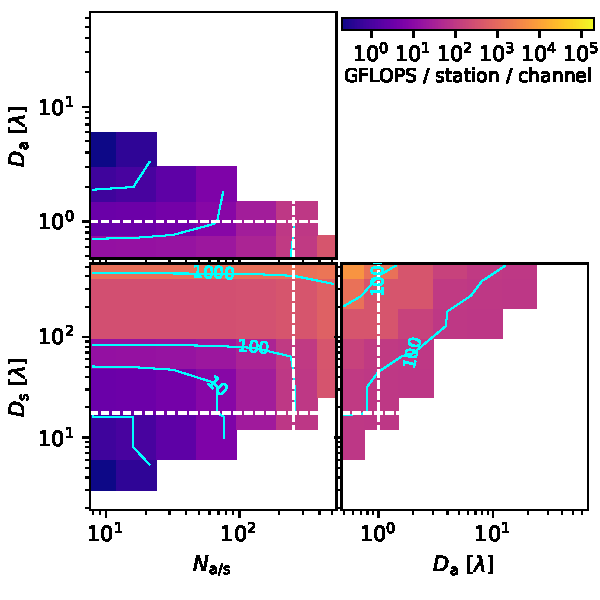
\includegraphics[width=0.48\textwidth]{figures/multidim_xcor_fft_cost_analysis_SKA1-low.pdf}}
% \subfloat[][Two-dimensional slices (relative)\label{fig:multidim-incoherent-relative-compcost-XFFT-SKA-low}]{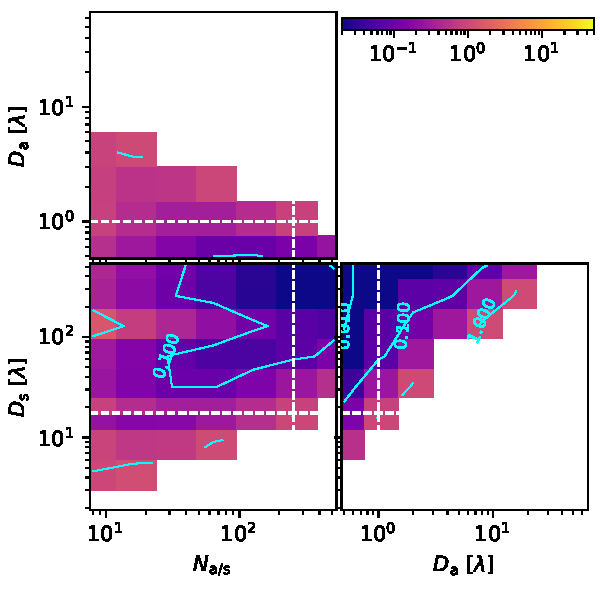
\includegraphics[width=0.48\textwidth]{figures/multidim_xcor_fft_relative_cost_analysis_SKA1-low.pdf}}
% \caption{(Left): Two-dimensional slices of the computational cost for coherent-incoherent imaging using an FFT of station-level cross-correlations for \texttt{SKA-low-core}, \texttt{SKA-low}, \texttt{Aus-VLBA-low}, and \texttt{IC-VLBA-low}. Cyan contours  \label{fig:incoherent-compcost-XFFT-SKA-low}}
% \end{figure*}

% \begin{figure}
% 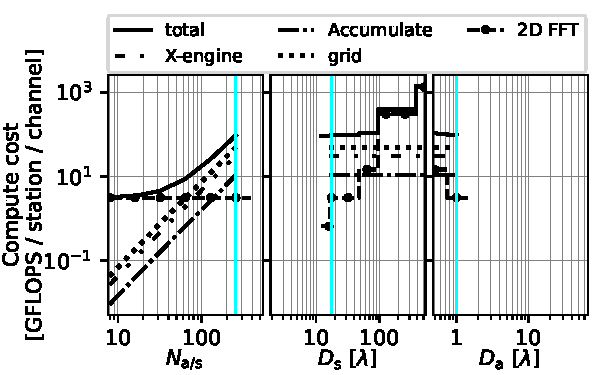
\includegraphics[width=\linewidth]{figures/1D_xcor_fft_cost_analysis_SKA1-low.pdf}
% % 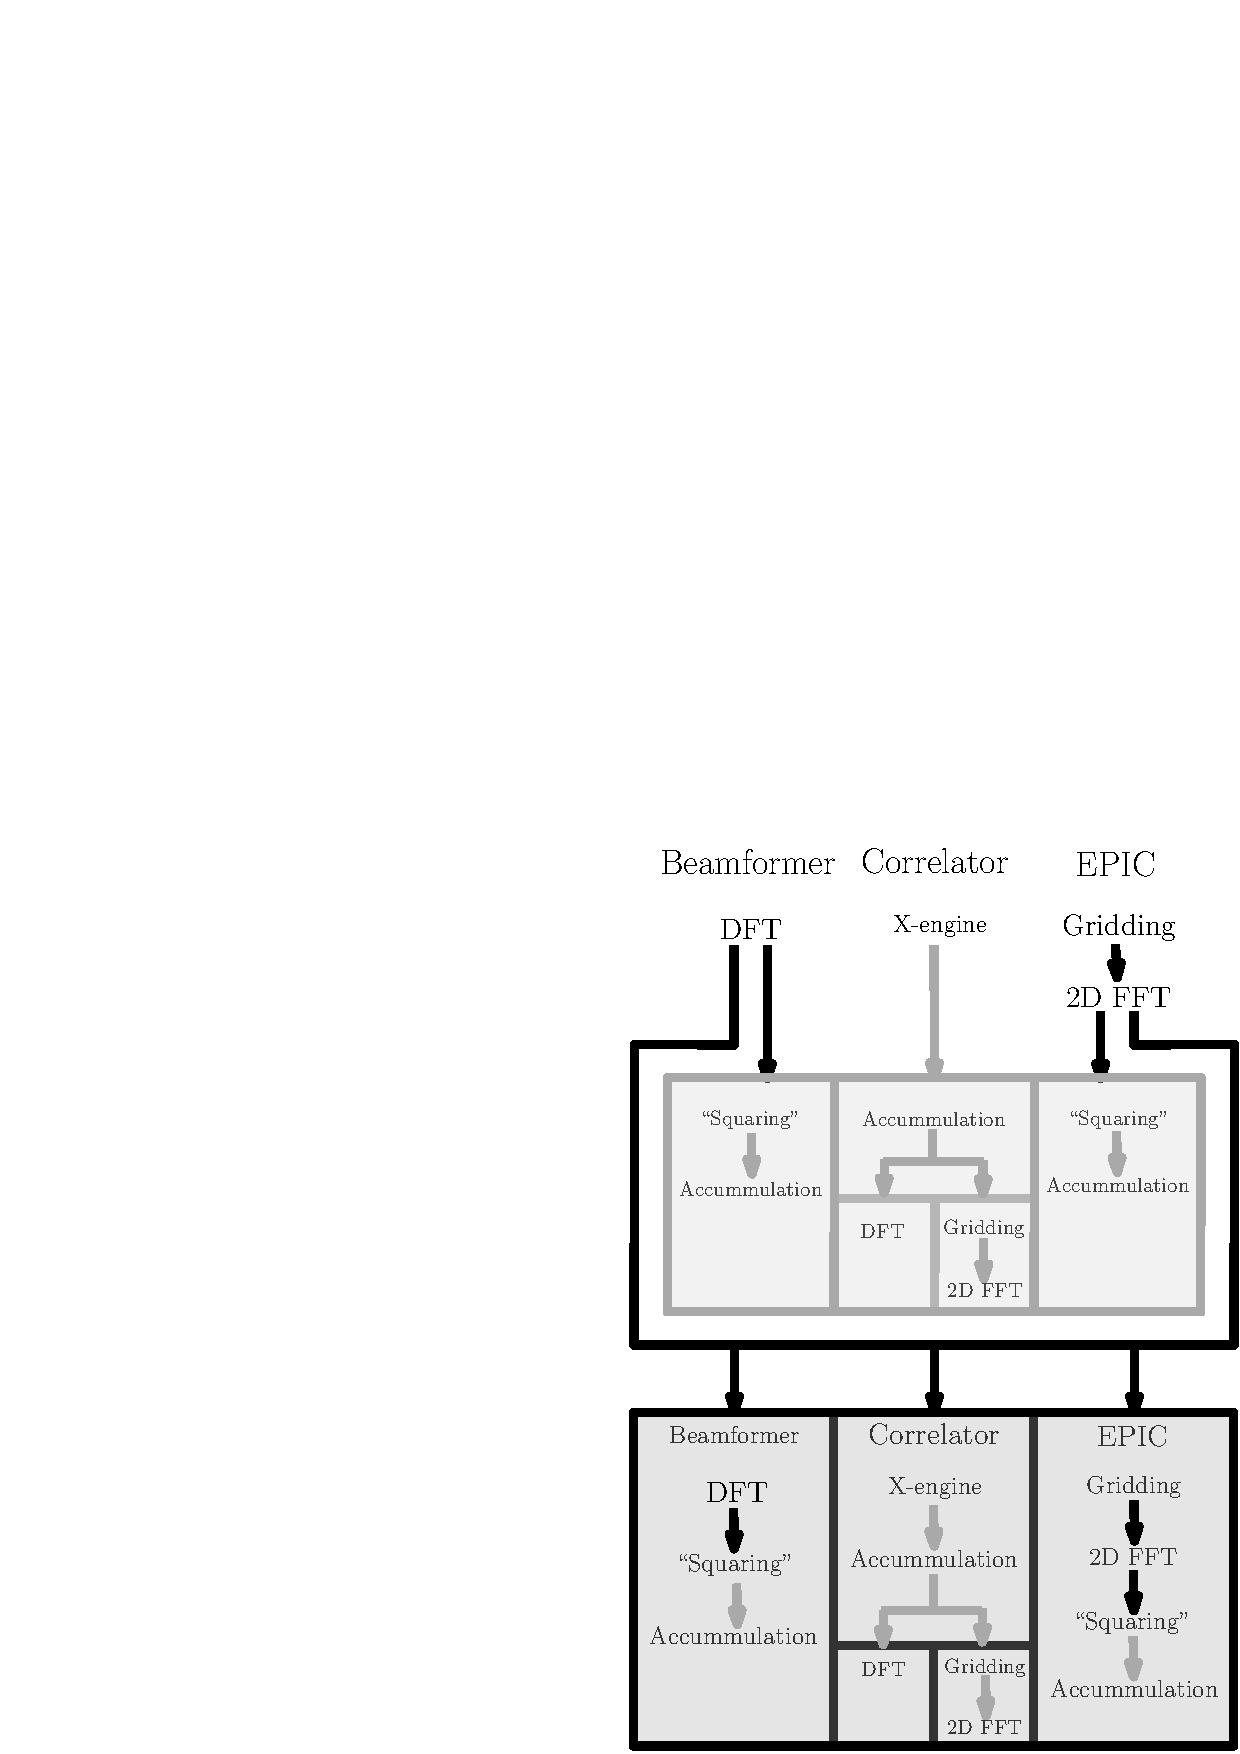
\includegraphics[width=\linewidth]{fig_01.pdf}
% \caption{
% \label{fig:1D-incoherent-compcost-XFFT-SKA-low}}
% \end{figure}

% \begin{figure}
% \centering
% \subfloat[][One-dimensional slices \label{fig:1D-incoherent-compcost-SKA-low}]{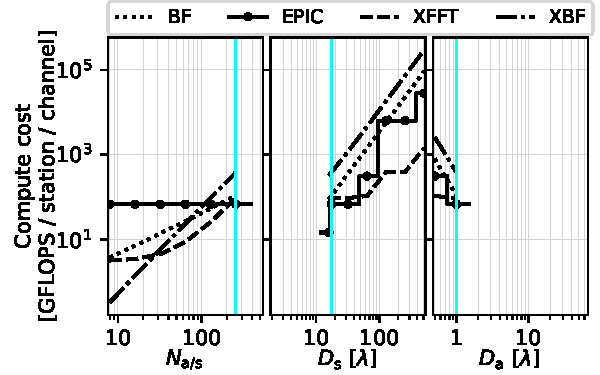
\includegraphics[width=\textwidth]{figures/1D_compcost_analysis_SKA1-low.pdf}} \\
% \subfloat[][One-dimensional slices (relative)\label{fig:1D-incoherent-compcost-XFFT-IC-VLBA-low}]{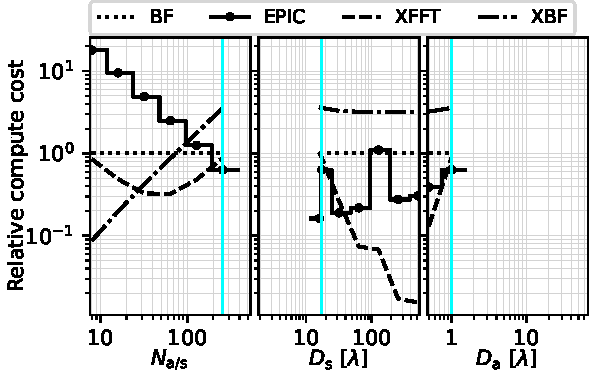
\includegraphics[width=\textwidth]{figures/1D_relative_compcost_analysis_SKA1-low.pdf}}
% \caption{(Left): One-dimensional slices of the computational cost for coherent-incoherent imaging using station-level voltage beamforming for \texttt{SKA-low-core}, \texttt{SKA-low}, \texttt{Aus-VLBA-low}, and \texttt{IC-VLBA-low}. Cyan contours  \label{fig:1D-incoherent-compcost-SKA-low}}
% \end{figure}

% \subsection{Stage II: Inter-station Architectures} \label{sec:inter-station-arch}

% \subsubsection{Incoherent Architectures} \label{sec:incoherent}

% \subsubsection{Coherent Architectures} \label{sec:coherent}

% \subsubsection{Beamforming -- Beamforming (1BF+2BF)}

% \subsubsection{Beamforming -- EPIC (1BF+2EPIC)}

% \subsubsection{Beamforming -- Correlator Beamforming (1BF+2XBF)}

% \subsubsection{Beamforming -- Correlation FFT (1BF+2XFFT)}

% \begin{figure*}
% 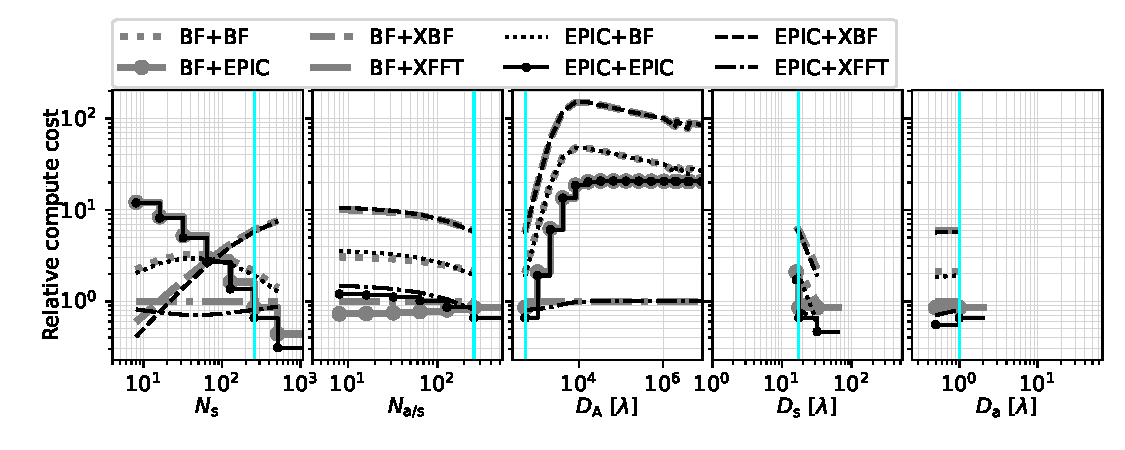
\includegraphics[width=0.95\textwidth]{figures/1D_coherent_relative_compcost_analysis_SKA1-low-core.pdf} 
% \caption{Computational cost of coherent strategy for \texttt{SKA-low-core} relative to BF+XFFT strategy. \label{fig:1D-coherent-relative-compcost-SKA-low-core}}
% \end{figure*}

% \begin{figure*}
% 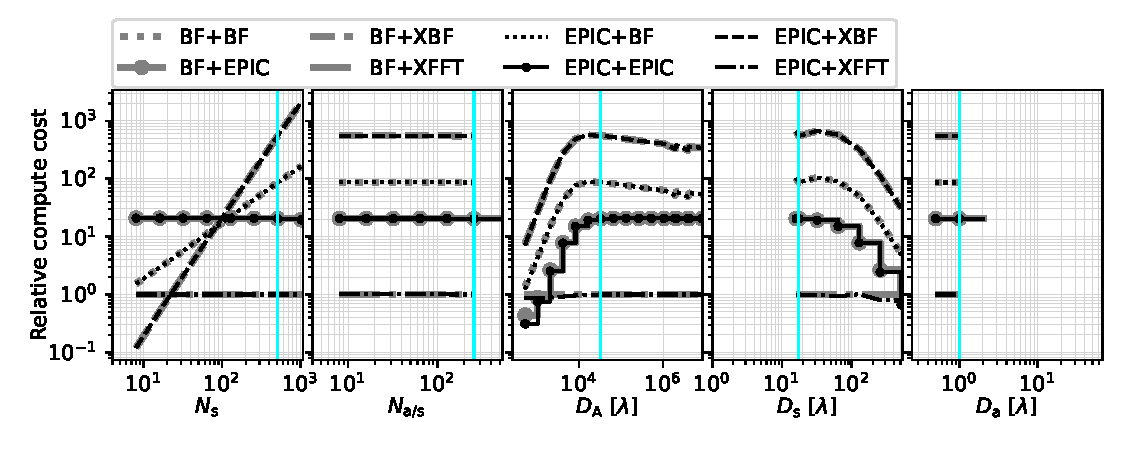
\includegraphics[width=0.95\textwidth]{figures/1D_coherent_relative_compcost_analysis_SKA1-low.pdf}
% \caption{Computational cost of coherent strategy for \texttt{SKA-low} relative to BF+XFFT strategy.  \label{fig:1D-coherent-relative-compcost-SKA-low}}
% \end{figure*}

% \begin{figure*}
% 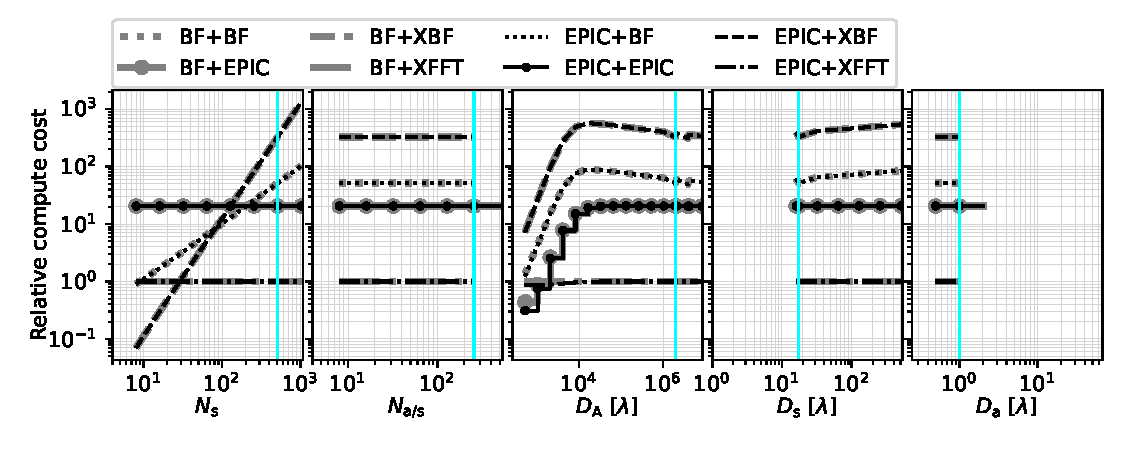
\includegraphics[width=0.95\textwidth]{figures/1D_coherent_relative_compcost_analysis_AU-VLBA-low.pdf}
% \caption{Computational cost of coherent strategy for \texttt{Aus-VLBA-low} relative to BF+XFFT strategy. \label{fig:1D-coherent-relative-compcost-Aus-VLBA-low}}
% \end{figure*}

% \begin{figure*}
% 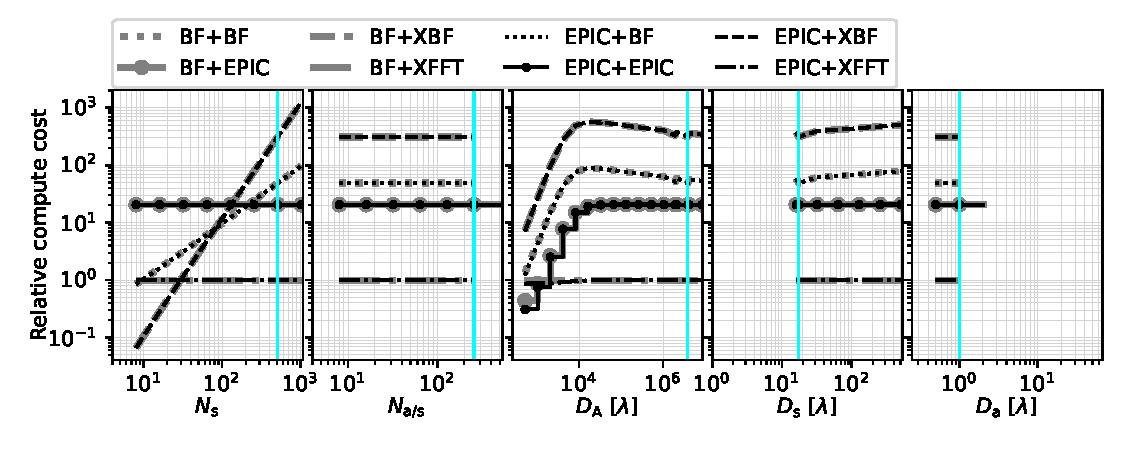
\includegraphics[width=0.95\textwidth]{figures/1D_coherent_relative_compcost_analysis_IC-VLBA-low.pdf}
% \caption{Computational cost of coherent strategy for \texttt{IC-VLBA-low} relative to BF+XFFT strategy. \label{fig:1D-coherent-relative-compcost-IC-VLBA-low}}
% \end{figure*}

\section{Results \& Discussion} \label{sec:results}

Below is a comparative view of the various architectures from the viewpoint of computational cost density for the range of array layouts and imaging cadence considered in this paper. 

\subsection{Station-scale Imaging Architectures}\label{sec:station-scale-imaging}

Figure~\ref{fig:1D-incoherent-compcost} shows a comparison of the computational cost densities of different imaging architectures discussed in section~\ref{sec:intra-station-arch} for varying parameters of the arrays in Table~\ref{tab:array_params}. The station layout parameters for \texttt{LAMBDA-I}, \texttt{SKA-low-core}, and \texttt{SKA-low} are identical, and thus so are their station-level computing costs. For these station parameters, EPIC holds a clear computational advantage. For \texttt{CASPA}, EPIC and XFFT hold the advantage for imaging cadence faster and slower than $t_\textrm{acc}\simeq 5$~ms, respectively, while for \texttt{FarView-core}, a similar tipping point between EPIC and XFFT occurs at a cadence of $t_\textrm{acc}\simeq 1$~ms.

\begin{figure}
\centering
\subfloat[][Station imaging compute cost densities for \texttt{LAMBDA-I}, \texttt{SKA-low}, and \texttt{SKA-low-core}. \label{fig:1D-incoherent-compcost-LAMBDA-I}]
{\includegraphics[width=\textwidth]
% {figures/1D_per_pixel_compcost_analysis_LAMBDA-I.pdf}
{fig_10a.pdf}
} \\
\subfloat[][Station imaging compute cost densities for \texttt{CASPA}.\label{fig:1D-incoherent-compcost-CASPA}]
{\includegraphics[width=\textwidth]
% {figures/1D_per_pixel_compcost_analysis_CASPA.pdf}
{fig_10b.pdf}
} \\
\subfloat[][Station imaging compute cost densities for \texttt{FarView-core}. \label{fig:1D-incoherent-compcost-FarView}]
{\includegraphics[width=\textwidth]
% {figures/1D_per_pixel_compcost_analysis_FarView.pdf}
{fig_10c.pdf}
}
\caption{Computational cost densities of different station-level imaging architectures for (a) \texttt{SKA-low-core}, \texttt{SKA-low}, and \texttt{LAMBDA-I}, (b) \texttt{CASPA}, and (c) \texttt{FarView-core}. In each subpanel, all parameters are fixed at the array's nominal value (cyan line) except the parameter shown on the $x$-axis. For \texttt{SKA-low-core}, \texttt{SKA-low}, and \texttt{LAMBDA-I}, the EPIC architecture is found to be most efficient computationally. For \texttt{CASPA}, EPIC is more efficient than other architectures when imaging cadence is $t_\textrm{acc}\lesssim 1-5$~ms, while XFFT is more efficient for $t_\textrm{acc}\gtrsim 5-10$~ms. For \texttt{FarView-core}, EPIC and XFFT are equally efficient when the cadence is $t_\textrm{acc}\approx 1$~ms, while EPIC and XFFT are advantageous for cadences faster and slower, respectively, than 1~ms.  \label{fig:1D-incoherent-compcost}}
\end{figure}

\subsection{Multi-scale Imaging Architectures}\label{sec:multi-scale-imaging}

Figure~\ref{fig:1D-coherent-compcost-a} shows a comparison of the compute cost densities in the discovery phase space of different multi-scale imaging architectures combining four options -- BF, EPIC, XBF, and XFFT -- on the inter-station data with two options -- BF and EPIC -- on the intra-station data for various array parameters and imaging cadences.  

\begin{figure*}
\centering
\subfloat[][\texttt{LAMBDA-I} \label{fig:1D-coherent-compcost-LAMBDA-I}]
{\includegraphics[width=\textwidth]
% {figures/1D_coherent_per_pixel_compcost_analysis_LAMBDA-I.pdf}
{fig_11a.pdf}
} \\
\subfloat[][\texttt{SKA-Low-core} \label{fig:1D-coherent-compcost-SKA-low-core}]
{\includegraphics[width=\textwidth]
% {figures/1D_coherent_per_pixel_compcost_analysis_SKA1-low-core.pdf}
{fig_11b.pdf}
} \\
\subfloat[][\texttt{SKA-Low} \label{fig:1D-coherent-compcost-SKA-low}]
{\includegraphics[width=\textwidth]
% {figures/1D_coherent_per_pixel_compcost_analysis_SKA1-low.pdf}
{fig_11c.pdf}
} 
\caption{One-dimensional slices of the computational cost density for (a) \texttt{LAMBDA-I}, (b) \texttt{SKA-low-core}, and (c) \texttt{SKA-low} using  coherent imaging at intra- and inter-station levels via BF (gray) and EPIC (black) for intra-station processing, and BF (dotted), EPIC (solid), XBF (dashed), and XFFT (dot-dashed) for inter-station processing of data. \label{fig:1D-coherent-compcost-a}}
\end{figure*}

\begin{figure*}\ContinuedFloat
\subfloat[][\texttt{CASPA} \label{fig:1D-coherent-compcost-CASPA}]
{\includegraphics[width=\textwidth]
% {figures/1D_coherent_per_pixel_compcost_analysis_CASPA.pdf}
{fig_11d.pdf}
} \\
\subfloat[][\texttt{FarView-core} \label{fig:1D-coherent-compcost-FarView}]
{\includegraphics[width=\textwidth]
% {figures/1D_coherent_per_pixel_compcost_analysis_FarView.pdf}
{fig_11e.pdf}
}
\caption{Contd. Same as above but for (d) \texttt{CASPA}, and (e) \texttt{FarView-core} \label{fig:1D-coherent-compcost-b}}
\end{figure*}

In all cases, EPIC (black lines) is more efficient than BF (gray lines) for intra-station full field of view data processing (first stage). This is because of the relatively large number of elements densely packed in stations and due to the capability of simultaneous full field of view beamforming by the EPIC architecture powered by the FFT's efficiency. 

The inter-station processing, however, varies significantly due to the diversity in the various inter-station array parameters and imaging cadence considered. For example, 
\begin{itemize}
    \item \texttt{LAMBDA-I} will benefit from deploying the correlator beamforming (XBF) architecture for inter-station processing by a factor of $\simeq 10$ over XFFT or BF. 
    \item \texttt{SKA-low-core} will have a marginal advantage from EPIC for the chosen parameters. However, if the number of stations, $N_\textrm{s}$, decreases,  the array diameter, $D_\textrm{A}$, increases or if the imaging cadence interval is slowed to $t_\textrm{acc} \gtrsim 5$~ms, the XFFT architecture starts to have a significant advantage over EPIC on the inter-station scale of data processing. 
    \item \texttt{SKA-low} will have an advantage from the XFFT architecture for inter-station processing by a factor $\simeq 20$.
    \item \texttt{CASPA} will have an advantage by a factor $\gtrsim 20$ from using the XBF architecture for inter-station processing due to significantly smaller number of stations.
    \item \texttt{FarView-core} appears to have a marginal advantage in using XFFT for inter-station processing for the chosen parameters. If $N_\textrm{s}$ increases or if the cadence interval decreases to $t_\textrm{acc}\lesssim 1$~ms, then EPIC becomes more efficient. 
\end{itemize}

\subsection{Effect of Imaging Cadence}\label{sec:cadence}

% The timescales of radio transients span many orders of magnitudes \citep{Pietka+2015,Chandra+2016,Nimmo+2022}. Pulsars, stellar bursts \citep{Zhang+2023}, and gamma ray burst afterglows, for example, are active on timescales from milliseconds to seconds, millisecond pulsars on milliseconds to tens of milliseconds, and FRBs on sub-milliseconds to tens of milliseconds \citep{Crawford+2022,Gupta+2022,Snelders+2023}. The exact origin of these energetic phenomena are yet to be fully understood. Extremely energetic and ultra-fast phenomena on timescales of sub-milliseconds such as magnetars and sub-millisecond pulsars \citep{Du+2009,Haskell+2018}, and on nanoseconds such as giant pulses from the Crab pulsar \citep{Hankins+2003,Hankins+2007,Eilek+2016,Philippov+2019}, for example, can reveal the fundamental nature of matter and exotic physics. 

The scientific goals enabled by access to \textbf{the wide range of timescales exhibited by transient phenomena (microseconds to days)} are key determinants of whether the architecture deployed can support the processing, as they are intricately tied to different timescales evident from Table~\ref{tab:intra-inter-station-coherent-imaging}. Here, the impact of the cadence interval on the choice of imaging architecture for multi-scale arrays for intra- and inter-station processing is examined. Table~\ref{tab:cadence} summarises the findings from Figures~\ref{fig:1D-incoherent-compcost} and \ref{fig:1D-coherent-compcost-b} based on the dependence of the computational cost densities of the different architectures and arrays on $t_\textrm{acc}$.

\begin{table*}[htb!]
\normalsize
\begin{threeparttable}
\caption{Impact of imaging cadence on choice of efficient imaging architecture.}
\label{tab:cadence}
% \begin{tabularx}{\textwidth}{ccccc}
\begin{tabular}{c|ccc|ccc}
\toprule
\headrow 
% Array & & Intra-station & & & Inter-station & \\
Array & \multicolumn{3}{c|}{Intra-station architecture} & \multicolumn{3}{c}{Inter-station architecture} \\ 
 & $\lesssim 0.1$~ms & $\simeq 1$~ms & $\gtrsim 100$~ms & $\lesssim 0.1$~ms & $\simeq 1$~ms & $\gtrsim 100$~ms \\ 
\midrule\midrule

\texttt{LAMBDA-I} & EPIC & EPIC & EPIC & BF/XBF & XBF & XBF \\
\midrule
\texttt{SKA-low-core} & EPIC & EPIC & EPIC & EPIC & EPIC & XFFT/EPIC/XBF \\
\midrule
\texttt{SKA-low} & EPIC & EPIC & EPIC & XFFT/EPIC & XFFT & XFFT \\
\midrule
\texttt{CASPA} & EPIC & EPIC & XFFT & XBF & XBF & XBF \\
\midrule
\texttt{FarView-core} & EPIC & EPIC & EPIC & EPIC & XFFT & XBF/XFFT \\
% \midrule
% Three & Four&three three\tnote{b} &four & & \\
\bottomrule
% \end{tabularx}
\end{tabular}
% \begin{tablenotes}[hang]
% % \item[]Table note
% \item[a]Array filling factor, $\,f_\textrm{A}=N_\textrm{s}\,(D_\textrm{s}/D_\textrm{A})^2$
% % \item[b]Station filling factor, $\,f_\textrm{s}=N_\textrm{eps}\,(D_\textrm{e}/D_\textrm{s})^2$
% \end{tablenotes}
\end{threeparttable}
\end{table*}

For intra-station processing, EPIC emerges as the most efficient among various architectures for all arrays considered on all timescales by a factor of $\lesssim 10$, except for \texttt{CASPA} when $t_\textrm{acc}\gtrsim 100$~ms where the XFFT architecture emerges to be more efficient than EPIC by a factor of few. This is because the stations having a sufficiently large number of elements packed densely is a notable aspect of all these arrays (see Table~\ref{tab:array_params}). For arrays like \texttt{CASPA} that have lesser number of elements and/or are not as densely packed, the cadence interval becomes an important factor. For cadence intervals, $t_\textrm{acc}\gtrsim 100$~ms, the XFFT architecture becomes advantageous.

The same reasoning can be extended for inter-station processing, where there is significant diversity. There is a large range in the number of stations and in the array filling factor. As a result, both the layout and cadence interval play significant roles in determining the efficiency of architectures. For arrays with small numbers of stations such as \texttt{LAMBDA-I} and \texttt{CASPA}, the XBF architecture holds an advantage by a factor of $\simeq 10$ on $t_\textrm{acc}\gtrsim 1$~ms and BF for $t_\textrm{acc}\lesssim 0.1$~ms. For arrays with large numbers of stations such as \texttt{SKA-low-core} with a reasonably high packing density, EPIC holds the advantage on all timescales by a factor of few, but with slower cadence intervals, $t_\textrm{acc}\gtrsim 100$~ms, XBF and XFFT also have comparable efficiency. Although the \texttt{SKA-low} has a large number of stations, they are not as densely packed as in the core, and therefore, the role of $t_\textrm{acc}$ is more significant. XFFT and EPIC are comparable (within a factor of few) at $t_\textrm{acc}\lesssim 1$~ms, but for $t_\textrm{acc}\gtrsim 1$~ms, XFFT is clearly efficient by a factor $\gtrsim 10$. Similarly, \texttt{FarView-core} has a comparable array filling factor as \texttt{SKA-low-core}, but has far fewer stations. Hence, EPIC is only marginally efficient for $t_\textrm{acc}\lesssim 0.1$~ms, whereas XFFT becomes more efficient by a factor of few for $t_\textrm{acc}\gtrsim 1$~ms. 

\subsection{Other considerations}\label{sec:other-metrics}

In transient search and cosmological applications, there will be additional processing required. For example, a de-dispersion trial process is required to discover new FRBs and pulsars with optimum signal-to-noise ratio. Computationally efficient algorithms for de-dispersion like the Fast Dispersion Measure Transform \citep[FDMT;][]{Zackay+2014} need to be performed either on intensities in the image plane pixels or on visibilities in the aperture plane, the cost of which will scale with the number of independent pixels in the image or the visibilities, respectively. For compact, dense, large-$N$ arrays, the number of independent pixels will be typically lesser than the number of measured visibilities, and thus it will be advantageous to perform de-dispersion in the image plane. Correspondingly, it will be computationally preferable to de-disperse visibilities for sparse arrays. A full accounting of such costs for most general cases is beyond the scope of this paper.
% on every independent pixel in the image formed. De-disperson may be performed 

In intensity mapping applications for cosmology, the images need to be post-processed for deconvolution, foreground, removal, etc. As these post-processing computations are additional and common to all architectures, including them in adopted cost metric will not affect the results. Calibration is another aspect that is not included in this computational cost analysis. Because calibration typically operates on a significantly slower cadence compared to $t_\textrm{acc}$, and the computational cost is not tedious \citep{Beardsley+2017,Gorthi+2021}, its contribution is negligible to the overall cost budget, and therefore will not affect the results.

Besides computational costs, there are other practical considerations in the deployment of an architecture such as the hardware's processing bandwidth, internal memory bandwidth management, input and output data rates, etc. For example, the GPU-based deployment of EPIC on the LWA is severely limited by the memory bandwidth constraints on chip\footnote{See \url{https://github.com/epic-astronomy/Memos/blob/master/PDFs/009_EPIC_Code_Optimizations.md} for a detailed analysis.}. The architecture of current generation of GPUs is found to be inefficient at handling the transpose operation required in an $N$-point two-dimensional FFT, whereas they may be more efficient at handling correlations. On the contrary, the current generation of FPGAs seem more suited for low bit width two-dimensional FFT from computational and on-chip memory bandwidth perspectives. It is extremely difficult to forecast the continually evolving landscape of hardware capabilities accessible to instruments at the instant of deployment. Thus, this analysis has been restricted to the metric of computational cost density, which is independent of evolving hardware capabilities. For example, even if the computations are parallelised over a large number of GPU cores as noted in \citet{Sokolowski+2024}, the total computational cost remains unaffected. So, it is intended to be viewed as a first step among many towards an actual implementation. 

% \subsection{SKA-low}

% \subsection{SKA-low Core}

% \subsection{CASPA}

% \subsection{FarView}

% \subsection{Australian VLBA-low}

% \subsection{Inter-continental VLBA-low}

\section{Conclusions} \label{sec:conclusion}

Explosive transient phenomena and observations of cosmological structures are two high impact science drivers in radio astronomy. The paradigm of aperture arrays used in radio astronomy is undergoing a transformation towards large numbers of low-cost elements grouped together in a hierarchy of spatial scales to achieve the desired science outcomes. Such a paradigm faces enormous challenges in computing and throughput because of the large numbers of elements spanning a multiplicity of spatial scales, a range of cadence intervals, real-time processing, and a continuous operation model. Different processing architectures are optimal for specific layouts and processing cadences. However, a single architectural may not be optimal for a hierarchical spatial layout.

This paper explores hybrid architecture solutions for existing and planned multi-scale aperture arrays (\texttt{SKA-low-core}, \texttt{SKA-low}, \texttt{LAMBDA-I}, \texttt{CASPA}, and \texttt{FarView-core}) on a wide range of cadence intervals, 0.1~ms$\le t_\textrm{acc} \le 10$~s, over the full field of view, using the metric of computational cost density evaluated over the discovery parameter space. The interferometric data processing architectures considered here are pre-correlation voltage beamformer (BF), a generic FFT-based direct imager (EPIC), beamforming from correlations (XBF), and FFT-based imaging of correlations (XFFT). The compute budget for various architecture combinations for these different arrays are broken down into their detailed components. 

For densely packed layouts with large numbers of elements, EPIC is computationally quite efficient regardless of processing cadence. This was the case for the station layouts of all the arrays considered, and hence EPIC emerges as the computationally most efficient architecture for full field of view, station level data processing on all cadence intervals except for \texttt{CASPA} on $t_\textrm{acc}\gtrsim 100$~ms, when XFFT becomes more efficient, although marginally. 
% Thus, in almost cases of station layouts considered here, EPIC appears to hold a clear advantage for full field of view, intra-station processing. 

The inter-station array layout has a wider range in the number of stations and density of their distribution. In such cases, the cadence interval plays a significant role in determining the computationally most efficient architecture. For inter-station data processing in \texttt{LAMBDA-I} and \texttt{CASPA}, XBF is found to be the most suitable option for all cadence intervals, while for \texttt{SKA-low-core} it is EPIC that holds the advantage on all cadence intervals. For \texttt{SKA-low}, XFFT appears most efficient for $t_\textrm{acc}\gtrsim 1$~ms, while EPIC and XFFT become comparable for $t_\textrm{acc}\lesssim 0.1$~ms. Thus, a multi-scale aperture array requires an optimal hybrid architecture strategy depending on the processing cadence, which in turn depends on the scientific objectives. This study provides a guide for designing computationally strategic data processing architecture for multi-scale aperture arrays, and conversely, can be used to design array parameters for specified computational complexity. 

This work considers only computational cost density over the discovery parameter space as a metric for finding the most efficient combination of processing architectures for multi-scale aperture arrays. Additional computing will be required for post-processing steps such as de-dispersion, deconvolution, etc. depending on the application. Actual deployment will have to take other significant practical factors into account such as power consumption, memory bandwidth, data rate, cost and capabilities of current hardware.

% See example table in Table~\ref{table_example}.

% \begin{table}[hbt!]
% \begin{threeparttable}
% \caption{An Example of a Table}
% \label{table_example}
% \begin{tabular}{llll}
% \toprule
% \headrow Column head 1 & Column head 2  & Column head 3 & Column head 4\\
% \midrule
% One\tnote{a} & Two&three three &four\\ 
% \midrule
% Three & Four&three three\tnote{b} &four\\
% \bottomrule
% \end{tabular}
% \begin{tablenotes}[hang]
% \item[]Table note
% \item[a]First note
% \item[b]Another table note
% \end{tablenotes}
% \end{threeparttable}
% \end{table}


% \section{Conclusion}
% The conclusion text goes here.


\begin{acknowledgement}
Inputs from Ron Ekers, Vivek Gupta, David Humphrey, Nivedita Mahesh, and Rajaram Nityananda are gratefully acknowledged. 
\end{acknowledgement}

% \paragraph{Funding Statement}

% This research was supported by grants from the <funder-name> <doi> (<award ID>); <funder-name> <doi> (<award ID>).

% \paragraph{Competing Interests}

% A statement about any financial, professional, contractual or personal relationships or situations that could be perceived to impact the presentation of the work --- or `None' if none exist.

% \paragraph{Data Availability Statement}

% A statement about how to access data, code and other materials allowing users to understand, verify and replicate findings --- e.g. Replication data and code can be found in Harvard Dataverse: \verb+\url{https://doi.org/link}+.

%\endnote in some journals will behave like \footnote; and \printendnotes will not output anything. 
\printendnotes

% \printbibliography
\bibliography{refs}

% \appendix

% \section{Mathematical Details}\label{sec:notation}

% Let $\mathcal{E}^\alpha_\nu(\hat{\boldsymbol{s}},t)$ represent the spectral Fourier components of the electric field time series emanating from astrophysical sources of emission in directions denoted by the unit vector, $\hat{\boldsymbol{s}}$, where, $\alpha\in\{1,2\}$ denotes the index of the polarisation state of the radiation, $\nu$ denotes the spectral component or the frequency of radiation, $\lambda=c/\nu$ is the wavelength, and $c$ is the speed of light. Hereafter, without loss of generality, all quantities can be implicitly assumed to depend on time and frequency throughout without explicit specification. Thus, $\mathcal{E}^\alpha(\hat{\boldsymbol{s}})\equiv \mathcal{E}^\alpha_\nu(\hat{\boldsymbol{s}},t)$

% Electric fields in the aperture plane, $E^\alpha(\boldsymbol{r})$, can be written as a superposition of those that propagated from the astrophysical sources on the celestial surface $\mathbb{S}$:
% \begin{align}
%     E^\alpha(\boldsymbol{r}) &= \int_\mathbb{S} \mathcal{E}^\alpha(\hat{\boldsymbol{s}})\, e^{-i \frac{2\pi}{\lambda}\hat{\boldsymbol{s}}\cdot\boldsymbol{r}} \,\mathrm{d}\Omega,
% \end{align}
% where, the integral is over the celestial surface, $\mathbb{S}$, covered by the unit vector, $\hat{\boldsymbol{s}}$, $\boldsymbol{r}$ denotes the observer's location, $\mathrm{d}\Omega=\mathrm{d}^2\hat{\boldsymbol{s}}$ is the infinitesimal solid angle element on $\mathbb{S}$ perpendicular to $\hat{\boldsymbol{s}}$. 

% The measuring instrument will imprint its transfer function on the measurements. If $a$ denotes a collecting element at location $\boldsymbol{r}_{a}$, then the electric field measured by this element will be
% \begin{align}
%     E_{a}^p &= \int_\mathbb{S} \sum_\alpha \mathcal{W}_{a}^{p\alpha}(\hat{\boldsymbol{s}})\, \mathcal{E}^\alpha(\hat{\boldsymbol{s}})\, e^{-i \frac{2\pi}{\lambda} \hat{\boldsymbol{s}}\cdot\boldsymbol{r}_{a}} \,\mathrm{d}\Omega + n_{a}^p \, , \label{eqn:polarimetric-Efield-element-ideal}
% \end{align}
% where, $n_{a}^p$ and $\mathcal{W}_{a}^{p\alpha}(\hat{\boldsymbol{s}})$ are the stochastic noise and polarisation-sensitive, directional electric field response of the element, $a$, respectively. $\mathcal{W}_{a}^{p\alpha}(\hat{\boldsymbol{s}})$ denotes the contribution from polarisation state, $\alpha$, in $\mathbb{S}$ to polarisation state, $p$, in the measurement.

% Thus, the measured electric field can be treated as a linear superposition of the electric fields emanating from astronomical sources with appropriate complex phases acquired on account of propagation and properties of the measuring instrument. Ignoring wide-field effects, this relation can be simplified as a two-dimensional Fourier transform of the electric fields in the sky coordinates \citep{TMS2017}. Using the convolution theorem of Fourier transform, Equation~(\ref{eqn:polarimetric-Efield-element-ideal}) can be expressed as the weighted integral of the propagated electric field over the region the element is responsive to in the aperture surface, $\mathbb{R}$, 
% \begin{align}
%     E_{a}^p &= \int_\mathbb{R} \sum_\alpha W_{a}^{p\alpha}(\boldsymbol{r}_{a} - \boldsymbol{r})\,E^\alpha(\boldsymbol{r}) \, \mathrm{d}^2 \boldsymbol{r}+ n_{a}^p \, , \label{eqn:polarimetric-Efield-element-ideal-aperture-continuous}
% \end{align}
% where, the weighting, denoted by $W_{a}^{p\alpha}(\boldsymbol{r})$, is the spatial Fourier transform of $\mathcal{W}_{a}^{p\alpha}(\hat{\boldsymbol{s}})$,
% \begin{align}
%     W_{a}^{p\alpha}(\boldsymbol{r}) &= \frac{1}{\lambda^2}\int_\mathbb{S} \mathcal{W}_{a}^{p\alpha}(\hat{\boldsymbol{s}})\, e^{-i\frac{2\pi}{\lambda} \hat{\boldsymbol{s}}\cdot \boldsymbol{r}} \,\mathrm{d}\Omega \, . \label{eqn:holographic-Efield-illumination}
% \end{align}

% Equation~(\ref{eqn:polarimetric-Efield-element-ideal-aperture-continuous}) involves a weighted integral of the propagated electric fields, where the weighting corresponds to the instrumental response, $W_{a}^{p\alpha}(\boldsymbol{r})$, centred at the location of the element, $a$, in the aperture plane, $\mathbb{R}$. Generally, $W_{a}^{p\alpha}(\boldsymbol{r})$ is physically interpretable as the holographic pattern of the element element in the aperture plane, which has support over the element's area of influence where it collects signals from. 
% % However, in some cases such as for narrow dipoles, this relation is purely mathematical and a physical interpretation is not straightforward. 
% % such as narrow dipoles, this relation is  encapsulates the aperture field illumination pattern of the element or the element's aperture distribution, 
% $W_{a}^{p\alpha}(\boldsymbol{r})$ can also include other instrumental effects that influence the element behavior. 

% Equations~(\ref{eqn:polarimetric-Efield-element-ideal}) and (\ref{eqn:polarimetric-Efield-element-ideal-aperture-continuous}) can be discretised as:
% \begin{align}
%     E_{a}^p &= \sum_k e^{-i\frac{2\pi}{\lambda}\hat{\boldsymbol{s}}_k\cdot\boldsymbol{r}_{a}} \, \sum_\alpha \left[\mathcal{W}_{a}^{p\alpha}(\hat{\boldsymbol{s}}_k) \, \mathcal{E}^\alpha(\hat{\boldsymbol{s}}_k)\right] \, \delta\Omega_k + n_{a}^p \, , \label{eqn:Efield-element-img-discrete}
% \end{align}
% or
% \begin{align}
%     E_{a}^p &= \sum_j \sum_\alpha W_{a}^{p\alpha}(\boldsymbol{r}_{a}-\boldsymbol{r}_j)\, \delta^2\boldsymbol{r}_j \left(\sum_k e^{-i\frac{2\pi}{\lambda} \hat{\boldsymbol{s}}_k\cdot\boldsymbol{r}_j} \, \mathcal{E}^\alpha(\hat{\boldsymbol{s}}_k) \,\delta\Omega_k \right) \nonumber\\ 
%     &\quad + n_{a}^p \, , \label{eqn:Efield-element-aperture-discrete}    
% \end{align}
% respectively. Equation~(\ref{eqn:Efield-element-aperture-discrete}) can be represented linear algebraically as
% \begin{align}
%     \mathbf{E}_{[p,\boldsymbol{r}_{a}]} &= \mathbf{W}_{[p,\boldsymbol{r}_{a}\leftarrow \alpha,\boldsymbol{r}]} \, \mathbf{F}_{[\boldsymbol{r}\leftarrow \hat{\boldsymbol{s}}]} \, \boldsymbol{\mathcal{E}}_{[\alpha,\hat{\boldsymbol{s}}]} + \mathbf{n}_{[p,\boldsymbol{r}_{a}]} \, .
% \end{align}
% The subscripted variables on either side of $\leftarrow$ indicate the transformation carried out by the associated matrix. For example, $\mathbf{F}_{[\boldsymbol{r}\leftarrow \hat{\boldsymbol{s}}]}\coloneqq e^{-i\frac{2\pi}{\lambda} \hat{\boldsymbol{s}}_k\cdot\boldsymbol{r}_j}$ denotes the Fourier matrix transforming variables defined on sky grid, $\hat{\boldsymbol{s}}_k$, to the aperture grid, $\boldsymbol{r}_j$. And, $\mathbf{W}_{[p,\boldsymbol{r}_{a}\leftarrow \alpha,\boldsymbol{r}]}\coloneqq \{W_{a}^{p\alpha}(\boldsymbol{r}_{a}-\boldsymbol{r}_j)\}$ is a matrix, where each row corresponds to the holographic pattern of an element, $W_{a}^{p\alpha}(\boldsymbol{r}_j)$, and the columns correspond to the aperture grid locations, $\boldsymbol{r}_j$. In each row, the holographic weights are shifted to the element location, $\boldsymbol{r}_{a}$. 

% The theory of mutual coherence has established the relation between the intensity distribution of spatially incoherent quasi-monochromatic emission, $I^{\alpha\beta}(\hat{\boldsymbol{s}})\coloneqq \bigl\langle \mathcal{E}^\alpha(\hat{\boldsymbol{s}}) \mathcal{E}^{\beta *}(\hat{\boldsymbol{s}}) \bigr\rangle$ on $\mathbb{S}$ and mutual coherence, or visibility, $V^{\alpha\beta}(\Delta\boldsymbol{r})\coloneqq \bigl\langle E^\alpha(\boldsymbol{r})E^{\beta *}(\boldsymbol{r}+\Delta\boldsymbol{r})\bigr\rangle$, in the aperture plane, and is popularly known as the \textit{Van Cittert-Zernike} theorem \citep{VanCittert1934,Zernike1938,Born-Wolf,Goodman2000,TMS2017}:
% \begin{align}
%     V^{\alpha\beta}(\Delta\boldsymbol{r}) &= \int_\mathbb{S} \mathcal{I}^{\alpha\beta}(\hat{\boldsymbol{s}})\, e^{-i\frac{2\pi}{\lambda} \hat{\boldsymbol{s}}\cdot\Delta\boldsymbol{r}} \,\mathrm{d}\Omega, \label{eqn:VCZ-theorem}
% \end{align}
% where, $\Delta\boldsymbol{r}$, denotes the displacement vector between any two locations\footnote{The dependence of spatial coherence on $\Delta\mathbb{R}$ (displacement vectors between the element pairs), rather than $\mathbb{R}$ (absolute positions), in Equation~(\ref{eqn:VCZ-theorem}) implies an assumption of wide-sense spatial stationarity for the electric fields measured on the aperture, which will hold true only when the spatial intensity distribution, $\mathcal{I}^{\alpha\beta}(\hat{\boldsymbol{s}})$, on $\mathbb{S}$ is spatially incoherent.} in the aperture domain $\mathbb{R}$, $\langle\cdot\rangle$ denotes an estimator of the ensemble average\footnote{This is typically obtained by assuming ergodicity and averaging over a coherence scale usually along temporal or spectral axes, and sometimes over redundant element spacings.}, and $*$ denotes complex conjugation. When the instrument's transfer function is included in the measurement process, the visibility measured by the interferometer elements $a$ and $b$ (with separation $\Delta\boldsymbol{r}_{ab}\coloneqq \boldsymbol{r}_{a}-\boldsymbol{r}_{b}$) will be:
% \begin{align}
%     V_{ab}^{pq} &= \int_\mathbb{S} \sum_{\alpha,\beta} \mathcal{B}_{ab}^{pq;\alpha\beta}(\hat{\boldsymbol{s}})\,\mathcal{I}^{\alpha\beta}(\hat{\boldsymbol{s}})\, e^{-i\frac{2\pi}{\lambda} \hat{\boldsymbol{s}}\cdot\Delta\boldsymbol{r}_{ab}} \,\mathrm{d}\Omega + n_{ab}^{pq} \, , \label{eqn:ideal-polarimetric-visibilities}
% \end{align}
% where, 
% \begin{align}
%     \mathcal{B}_{ab}^{pq;\alpha\beta}(\hat{\boldsymbol{s}}) &=  \mathcal{W}_{a}^{p\alpha}(\hat{\boldsymbol{s}}) \mathcal{W}_{b}^{{q\beta }^*}(\hat{\boldsymbol{s}}) \, ,
% \end{align}
% is the directional polarimetric cross-power pattern of an ideal two-element interferometer (made of elements $a$ and $b$) measuring two polarizations, $p$ and $q$. Equation~(\ref{eqn:ideal-polarimetric-visibilities}) is the polarimetric radio interferometric measurement equation (RIME).  
% % In the absence of other non-ideal effects, $\mathcal{B}_{a_m b_m}(\hat{\boldsymbol{s}})$ corresponds to the directional cross-power pattern of the interferometer comprising of elements $a$ and $b$.

% From the Fourier transform relations, the above equations can be expressed equivalently in the aperture plane. The cross-power illumination of the interferometer's aperture, $B_{ab}^{pq;\alpha\beta}(\Delta\boldsymbol{r})$, is the Fourier transform of the directional cross-power pattern, $\mathcal{B}_{ab}^{pq;\alpha\beta}(\hat{\boldsymbol{s}})$,
% \begin{align}
%     B_{ab}^{pq;\alpha\beta}(\Delta\boldsymbol{r}) &= \frac{1}{\lambda^2}\int_\mathbb{S} \mathcal{B}_{ab}^{pq;\alpha\beta}(\hat{\boldsymbol{s}}) \, e^{-i\frac{2\pi}{\lambda} \hat{\boldsymbol{s}}\cdot \Delta\boldsymbol{r}_{ab}} \,\mathrm{d}\Omega \label{eqn:holographic-power-illumination} \\
%     &= \int_\mathbb{R} W_{a}^{p\alpha}(\boldsymbol{r}) \, W_{b}^{q\beta *}(\boldsymbol{r}+\Delta\boldsymbol{r})\,\mathrm{d}^2\boldsymbol{r} \, ,
% \end{align}
% % In the aperture (Fourier) domain, it is equivalent to
% % \begin{align}
% %     B_{a_m b_m}^{pq;\alpha\beta}(\Delta\boldsymbol{r}) &= \int_\mathbb{R} W_{a_m}(\boldsymbol{r}) W_{b_m}^{*}(\boldsymbol{r}+\Delta\boldsymbol{r})\,\mathrm{d}^2\boldsymbol{r} \, ,
% % \end{align}
% which is a correlation of the aperture-plane responses of the two individual elements of the interferometer. The RIME in Equation~(\ref{eqn:ideal-polarimetric-visibilities}) can be expressed alternatively in the aperture domain as:
% \begin{align}
%     V_{ab}^{pq} &= \bigl\langle E_{a}^p \, E_{b}^{q*}\bigr\rangle\\ 
%     &= \int_{\Delta\mathbb{R}} \sum_{\alpha,\beta} B_{ab}^{pq;\alpha\beta}(\Delta\boldsymbol{r}_{ab}-\Delta\boldsymbol{r})\,V^{\alpha\beta}(\Delta\boldsymbol{r})\,\mathrm{d}^2\Delta\boldsymbol{r}  + n_{ab}^{pq} \, , \label{eqn:vis-degridding}
% \end{align}
% whose discrete linear algebraic representation is
% \begin{align}
%     \mathbf{V}_{[pq,\Delta\boldsymbol{r}_{ab}]} &= \mathbf{B}_{[pq,\Delta\boldsymbol{r}_{ab}\leftarrow \alpha\beta,\Delta\boldsymbol{r}]} \, \mathbf{F}_{[\Delta\boldsymbol{r}\leftarrow \hat{\boldsymbol{s}}]} \, \boldsymbol{\mathcal{I}}_{[\alpha\beta,\hat{\boldsymbol{s}}]} + \mathbf{n}_{[pq,\Delta\boldsymbol{r}_{ab}]} \, .
% \end{align}
% Equation~(\ref{eqn:vis-degridding}) represents a weighting of the true spatial coherence of the incident radiation by the interferometer's cross-power illumination pattern and integration over the region the interferometer has a response to, centered at $\Delta\boldsymbol{r}_{ab}$. $\Delta\mathbb{R}$ denotes the space of all possible displacement vectors between elements. 

% \section{Mathematical Details of Architectures}

% \subsection{Co-polar Interferometry}\label{sec:copolar-interferometry}

% If we represent $\mathcal{E}^\alpha(\hat{\boldsymbol{s}},\nu,t)$ as the spectral Fourier components, $\nu$, of the time-domain electric fields, $\mathcal{E}_{t^\prime}(\alpha,\hat{\boldsymbol{s}},t^\prime)$, emanating from astrophysical sources of emission in directions denoted by the unit vector, $\hat{\boldsymbol{s}}$ measured over a finite time interval, $T$, centered around time, $t$, then:
% \begin{align}
%     \mathcal{E}^\alpha(\hat{\boldsymbol{s}},\nu,t) = \frac{1}{T}\int\limits_{t-T/2}^{t+T/2} \mathcal{E}_{t^\prime}^\alpha(\hat{\boldsymbol{s}},t^\prime) e^{-i 2\pi \nu t^\prime} \mathrm{d}t^\prime,
% \end{align}
% where, superscript $\alpha\in\{1,2\}$ denotes the polarisation state of the radiation, $\nu$ denotes the spectral component or the frequency of radiation, $\lambda=c/\nu$ is the wavelength, where $c$ is the speed of light. Because all the operations considered in this paper operate independently on each spectral channel, $\nu$, and time, $t$, we will hereafter assume implicit dependence on $\nu$ and $t$ throughout without explicitly specifying it. 

% A measuring instrument, like an antenna in an aperture array, in the aperture plane will measure the superposition of these electric fields as they propagate from the sky locations spanning the celestial surface, $\mathbb{S}$, while imprinting its transfer function, $\mathcal{W}_{a_m}^{p\alpha}(\hat{\boldsymbol{s}})$, as
% \begin{align}
%     \underline{E}_{a_m}^p &= \int_\mathbb{S} \sum_\alpha  \mathcal{W}_{a_m}^{p\alpha}(\hat{\boldsymbol{s}})\, \mathcal{E}^\alpha(\hat{\boldsymbol{s}})\, e^{-i \frac{2\pi}{\lambda} \hat{\boldsymbol{s}}\cdot\boldsymbol{r}_{a_m}} \,\mathrm{d}\Omega \, , \label{eqn:polarimetric-Efield-element-ideal}
% \end{align}


% Electric fields in the aperture plane, $\underline{E}(\boldsymbol{r})$, can be written as a superposition of those that propagated from the astrophysical sources on the celestial surface $\mathbb{S}$, $\mathcal{E}(\hat{\boldsymbol{s}})$:
% \begin{align}
%     \underline{E}(\boldsymbol{r}) &= \int_\mathbb{S} \mathcal{E}(\hat{\boldsymbol{s}})\, e^{-i \frac{2\pi}{\lambda}\hat{\boldsymbol{s}}\cdot\boldsymbol{r}} \,\mathrm{d}\Omega,
% \end{align}
% where, the integral is over the celestial surface, $\mathbb{S}$, covered by the unit vector, $\hat{\boldsymbol{s}}$, $\boldsymbol{r}$ denotes the observer's location, $t$ denotes time, $\mathrm{d}\Omega=\mathrm{d}^2\hat{\boldsymbol{s}}$ is the infinitesimal solid angle element on the tangent plane of the celestial sphere perpendicular to the unit vector $\hat{\boldsymbol{s}}$. 

% Thus, the propagated electric field can be construed as a linear superposition of the electric fields emanating from astronomical sources with appropriate complex phases acquired during the propagation. Ignoring wide-field effects, this relation can be simplified as a Fourier transform of the electric fields in the sky coordinates. 

% % In the presence of a directional response of an ideal instrument, which includes but is not limited to the directional electric field pattern of the element, the electric field measured by the 

% In order to generalize later, we will consider a station indexed by $m$ as being made up of a group of $N_m$ elements, indexed by $a_m$. For now, we will focus on a single station, denoted by $m$. 

% The measuring instrument will imprint its transfer function on the measurements. If $\mathcal{W}_{a_m}(\hat{\boldsymbol{s}})$ is the directional electric field response of the element, $a_m$, then the electric field measured by this element will be ideally
% \begin{align}
%     \underline{E}_{a_m} &= \int_\mathbb{S} \mathcal{W}_{a_m}(\hat{\boldsymbol{s}})\, \mathcal{E}(\hat{\boldsymbol{s}})\, e^{-i \frac{2\pi}{\lambda} \hat{\boldsymbol{s}}\cdot\boldsymbol{r}_{a_m}} \,\mathrm{d}\Omega \, . \label{eqn:copolar-Efield-element-ideal}
% \end{align}
% In the typical case of non-ideal behavior of an element, the measured electric field will be potentially corrupted both in amplitude and phase relative to the ideal measurement in Equation~(\ref{eqn:copolar-Efield-element-ideal}). Then,
% \begin{align}
%     E_{a_m} &= g_{a_m}\underline{E}_{a_m} + n_{a_m} \, , \label{eqn:Efield-element}
% \end{align}
% where, $g_{a_m}$ denotes the multiplicative complex gain encapsulating the corruption of the wavefront due to instrumental and propagation effects, and $n_{a_m}$ denotes element-based additive noise in the measurement chain. A process of calibration is typically performed to remove the effects of this corruption by obtaining the best estimate, $\widehat{g}_{a_m}$, of the corrupting gain term, $g_{a_m}$, and the estimated electric field at the element after calibration will be:
% \begin{align}
%     \widehat{\underline{E}}_{a_m} &= \widehat{g}_{a_m}^{-1}\,E_{a_m} \, . \label{eqn:calibration}
% \end{align}


% % then $\mathcal{W}_{a_m}(\hat{\boldsymbol{s}})$ is the corresponding directional electric field response of the element. Thus, by application of Fourier transform properties, 
% % \begin{align}
% %     E_{a_m}^\textrm{I} &= \int_\mathbb{S} \mathcal{W}_{a_m}(\hat{\boldsymbol{s}})\, \mathcal{E}(\hat{\boldsymbol{s}})\, e^{-2\pi i\frac{\nu}{c} \boldsymbol{r}\cdot \hat{\boldsymbol{s}}} \,\mathrm{d}\Omega
% % \end{align}


% % \begin{align}
% %     &= \int_\mathbb{R} W_{a_m}(\boldsymbol{r} - \boldsymbol{r}_{a_m}) \nonumber\\
% %     &\quad \times \left[\int_\textrm{S} \mathcal{E}(\hat{\boldsymbol{s}})\, e^{-2\pi i\nu \boldsymbol{r}\cdot \hat{\boldsymbol{s}}/c} \,\mathrm{d}\Omega\right]\, \mathrm{d}^2 \boldsymbol{r} + n_{a_m} \\
% %     &= \int_\textrm{S} \mathcal{W}_{a_m}(\hat{\boldsymbol{s}})\, \mathcal{E}(\hat{\boldsymbol{s}})\, e^{-2\pi i\nu \boldsymbol{r}\cdot \hat{\boldsymbol{s}}/c} \,\mathrm{d}\Omega \nonumber\\ 
% %     &\qquad + n_{a_m}  + n_{a_m}
% % \end{align}
% % The weighting, denoted by $W_{a_m}(\boldsymbol{r})$, encapsulates the aperture field illumination pattern of the element, the complex element gains (including direction-dependence) containing the effects of the propagation medium as well as of the instrumentation. $\mathcal{W}_{a_m}(\hat{\boldsymbol{s}})$ is the spatial Fourier transform of $W_{a_m}(\boldsymbol{r})$. If $W_{a_m}(\boldsymbol{r})$ denotes only the aperture field illumination pattern, then $\mathcal{W}_{a_m}(\hat{\boldsymbol{s}})$ is the corresponding directional element voltage response towards the celestial surface. 

% The theory of mutual coherence has established the relation between the intensity distribution of spatially incoherent quasi-monochromatic emission, $I(\hat{\boldsymbol{s}})$ on $\mathbb{S}$ and mutual coherence, or ``true'' visibility, $\underline{V}(\Delta\boldsymbol{r})\coloneqq \bigl\langle \underline{E}(\boldsymbol{r})\underline{E}^*(\boldsymbol{r}+\Delta\boldsymbol{r})\bigr\rangle$, in the aperture plane, and is popularly known as the \textit{Van Cittert-Zernike} theorem \citep{VanCittert1934,Zernike1938,Born-Wolf,Goodman2000,TMS2017}:
% \begin{align}
%     \underline{V}(\Delta\boldsymbol{r}) &= \int_\mathbb{S} \mathcal{I}(\hat{\boldsymbol{s}})\, e^{-i\frac{2\pi}{\lambda} \hat{\boldsymbol{s}}\cdot\Delta\boldsymbol{r}} \,\mathrm{d}\Omega, \label{eqn:VCZ-theorem}
% \end{align}
% where, $\Delta\boldsymbol{r}$, denotes the displacement vector between any two locations\footnote{The dependence of spatial coherence on $\Delta\mathbb{R}$ (displacement vectors between the element pairs), rather than $\mathbb{R}$ (absolute positions), in Equation~(\ref{eqn:VCZ-theorem}) implies an assumption of wide-sense spatial stationarity for the electric fields measured on the aperture, which will hold true only when the spatial intensity distribution, $\mathcal{I}(\hat{\boldsymbol{s}})$, on $\mathbb{S}$ is incoherent.} in the aperture domain $\mathbb{R}$, $\langle\cdot\rangle$ denotes an estimator of the ensemble average\footnote{This is typically obtained by assuming ergodicity and averaging over a coherence scale usually along temporal or spectral axes, and sometimes over redundant element spacings.}, and $*$ denotes complex conjugation. When the ideal instrument's transfer function is included in the measurement process, the visibility measured by the interferometer elements $a$ and $b$ (with separation $\Delta\boldsymbol{r}_{a_m b_m}\coloneqq \boldsymbol{r}_{a_m}-\boldsymbol{r}_{b_m}$) will be:
% \begin{align}
%     \underline{V}_{a_m b_m} &= \int_\mathbb{S} \mathcal{B}_{a_m b_m}(\hat{\boldsymbol{s}})\,\mathcal{I}(\hat{\boldsymbol{s}})\, e^{-i\frac{2\pi}{\lambda} \hat{\boldsymbol{s}}\cdot\Delta\boldsymbol{r}_{a_m b_m}} \,\mathrm{d}\Omega, \label{eqn:ideal-copolar-visibilities}
% \end{align}
% where, 
% \begin{align}
%     \mathcal{B}_{a_m b_m}(\hat{\boldsymbol{s}}) &=  \mathcal{W}_{a_m}(\hat{\boldsymbol{s}})\,\mathcal{W}_{b_m}^*(\hat{\boldsymbol{s}}) \, ,
% \end{align}
% is called the directional cross-power pattern of an ideal two-element interferometer (made of elements $a$ and $b$). Equation~(\ref{eqn:ideal-copolar-visibilities}) is referred to as the radio interferometric measurement equation (RIME). 
% % In the absence of other non-ideal effects, $\mathcal{B}_{a_m b_m}(\hat{\boldsymbol{s}})$ corresponds to the directional cross-power pattern of the interferometer comprising of elements $a$ and $b$.

% Correlators in interferometer arrays produce complex correlations products of the measured (corrupted) electric fields between pairs of elements (denoted by $a$ and $b$) to produce corrupted visibilities,
% \begin{align}
%     V_{a_m b_m} &= \bigl\langle E_{a_m} \, E_{b_m}^*\bigr\rangle \\
%     &= g_{a_m}\, \underline{V}_{a_m b_m}\, g_{b_m}^* + n_{a_m b_m} \, . \label{eqn:corrupted-noise-visibility}
% \end{align}
% % where, $\underline{V}_{a_m b_m}$ denotes ideal visibilities measured at element spacing $\boldsymbol{r}_{a_m b_m}\coloneqq \boldsymbol{r}_{a_m}-\boldsymbol{r}_{b_m}$, $\langle\cdot\rangle$ denotes an estimator of the ensemble average\footnote{This is typically obtained by assuming ergodicity and averaging over a coherence scale usually along temporal or spectral axes, and sometimes over redundant element spacings.}, and $*$ denotes complex conjugation. 
% The corresponding estimate of ideal visibilities, after calibration, will be
% \begin{align}
%     \widehat{\underline{V}}_{a_m b_m} &= \bigl\langle \widehat{\underline{E}}_{a_m}\widehat{\underline{E}}_{b_m}^*\bigr\rangle \nonumber\\
%     &= \widehat{g}_{a_m}^{-1}\, V_{a_m b_m}\, \widehat{g}_{b_m}^{*^{-1}} \, .
% \end{align}
% Because this paper does not concern primarily with calibration, we will assume that the measured element electric fields are perfectly calibrated hereafter, and hence, $\widehat{\underline{E}}_{a_m}=\underline{E}_{a_m}$ and $E_{a_m}=\underline{E}_{a_m}+n_{a_m}$. Correspondingly, we will assume $\widehat{\underline{V}}_{a_m b_m}=\underline{V}_{a_m b_m}$ and $V_{a_m b_m}=\underline{V}_{a_m b_m}+n_{a_m b_m}$. 

% % Equation~(\ref{eqn:ideal-copolar-visibilities}) can be alternatively expressed in the aperture domain, using Fourier transform properties, as:
% % \begin{align}
% %     V_{a_m b_m}^\textrm{I} &= \int_{\Delta\mathbb{R}} B_{a_m b_m}(\Delta\boldsymbol{r}-\Delta\boldsymbol{r}_{a_m b_m})\,V^\textrm{T}(\Delta\boldsymbol{r})\,\mathrm{d}^2\Delta\boldsymbol{r}, \label{eqn:vis-degridding}
% % \end{align}
% % where, $B_{a_m b_m}(\Delta\boldsymbol{r})$ denotes the cross-power illumination of the interferometer's aperture. Equation~(\ref{eqn:vis-degridding}) represents a weighting of the true spatial coherence of the incident radiation by the interferometer's cross-power illumination pattern and integration over the region the interferometer has a response to. $\Delta\mathbb{R}$ denotes the space of all possible displacement vectors between elements. $B_{a_m b_m}(\Delta\boldsymbol{r})$ is the Fourier transform of $\mathcal{B}_{a_m b_m}(\hat{\boldsymbol{s}})$. Thus,
% % \begin{align}
% %     B_{a_m b_m}(\Delta\boldsymbol{r}) &= \frac{\nu^2}{c^2}\int_\mathbb{S} \mathcal{W}_{a_m}(\hat{\boldsymbol{s}})\mathcal{W}_{b_m}^{*}(\hat{\boldsymbol{s}})\nonumber\\
% %     &\qquad\qquad \times e^{-2\pi i\frac{\nu}{c} \Delta\boldsymbol{r}\cdot\hat{\boldsymbol{s}}} \,\mathrm{d}\Omega \\
% %     &= \int_\mathbb{R} W_{a_m}(\boldsymbol{r}) W_{b_m}^{*}(\boldsymbol{r}+\Delta\boldsymbol{r})\,\mathrm{d}^2\boldsymbol{r}. \label{eqn:holographic-power-illumination}
% % \end{align}
 
% % Interferometric image synthesis involves inverting Equation~(\ref{eqn:VCZ-theorem}) to obtain $\mathcal{I}(\hat{\boldsymbol{s}})$, the spatial intensity distribution on $\mathbb{S}$, using a number of calibrated visibility measurements, $\widehat{V}_{a_m b_m}$, from different element pairs. The optimal map-making (OMM) formalism \citep{Tegmark1997a} provides an optimal solution, which in the radio interferometric context is often referred to as the ``dirty image'' \citep{TMS2017,SIRA-II}. In linear algebraic notation, the measurement and the optimal inversion operations can be written as \citep{Bhatnagar+2008,Morales+2009}:
% % \begin{align}
% %     \mathbf{V}_{[\Delta\boldsymbol{r}_{a_m b_m}]} &= \mathbf{B}_{[\Delta\boldsymbol{r}_{a_m b_m}|\Delta\boldsymbol{r}]}\,\mathbf{F}_{[\Delta\boldsymbol{r}|\hat{\boldsymbol{s}}]}\,\mathbf{I}_{[\hat{\boldsymbol{s}}]} + \mathbf{n}_{[\Delta\boldsymbol{r}_{a_m b_m}]}, \label{eqn:RIME-LA}
% % \end{align}
% % and
% % \begin{align}
% %     \widehat{\mathbf{I}}_{[\hat{\boldsymbol{s}}]} &=  \mathbf{F}^\textrm{H}_{[\hat{\boldsymbol{s}}\leftarrow\Delta\boldsymbol{r}]}\,\mathbf{B}^\textrm{H}_{[\Delta\boldsymbol{r}\leftarrow\Delta\boldsymbol{r}_{a_m b_m}]}\,\mathbf{N}^{-1}_{[\Delta\boldsymbol{r}_{a_m b_m}\leftarrow\Delta\boldsymbol{r}_{a_m b_m}]}\,\widehat{\mathbf{V}}_{[\Delta\boldsymbol{r}_{a_m b_m}]} \label{eqn:OptEst-LA} \\
% %     &= \mathbf{F}^\textrm{H}_{[\hat{\boldsymbol{s}}\leftarrow\Delta\boldsymbol{r}]}\,\mathbf{B}^\textrm{H}_{[\Delta\boldsymbol{r}\leftarrow\Delta\boldsymbol{r}_{a_m b_m}]}\,\mathbf{N}^{-1}_{[\Delta\boldsymbol{r}_{a_m b_m}\leftarrow\Delta\boldsymbol{r}_{a_m b_m}]} \nonumber\\ 
% %     &\qquad\qquad\qquad \vect\left(\Bigl\langle\widehat{\mathbf{E}}_{[\boldsymbol{r}_{a_m}]}\widehat{\mathbf{E}}^\textrm{H}_{[\boldsymbol{r}_{b_m}]}\Bigl\rangle\right)_{[\Delta\boldsymbol{r}_{a_m b_m}]}, \label{eqn:opt-copolar-corr-image}
% % \end{align}
% % respectively. Here, the dependence on $\nu$ and $t$ have been omitted for convenience as they carry through the equation without transformations. $\vect(\mathbf{M})$ denotes the vectorization of a matrix $\mathbf{M}$ into a column vector. Quantities with a single bracketed variable, such as $\mathbf{V}_{[\Delta\boldsymbol{r}_{a_m b_m}]}$, $\mathbf{I}_{[\hat{\boldsymbol{s}}]}$, $\mathbf{n}_{[\Delta\boldsymbol{r}_{a_m b_m}]}$, and $\widehat{\mathbf{I}}_{[\hat{\boldsymbol{s}}]}$, denote vectors that are a function of that variable, and those with two bracketed variables denote matrix operators that transform the vector between the variable on the right of the delimiter $\leftarrow$ to that on its left. For example, Equation~(\ref{eqn:RIME-LA}) Fourier transforms a vector of true pixelized intensities, $\mathbf{I}_{[\hat{\boldsymbol{s}}]}$, to a spatial coherence function, $\mathbf{F}_{[\Delta\boldsymbol{r}|\hat{\boldsymbol{s}}]}\mathbf{I}_{[\hat{\boldsymbol{s}}]}$, defined on a continuous variable (or finely sampled in case of a discretized implementation), $\boldsymbol{r}_{a_m b_m}$, which through the operator represented by $\mathbf{B}_{[\Delta\boldsymbol{r}_{a_m b_m}|\Delta\boldsymbol{r}]}$ is then further transformed into a discrete vector of measured visibilities between specific element pairs, $\mathbf{V}_{[\Delta\boldsymbol{r}_{a_m b_m}]}$, which includes an additive measurement noise vector, $\mathbf{n}_{[\Delta\boldsymbol{r}_{a_m b_m}]}$. 
% % % weighted by $B_{a_m b_m}(\Delta\boldsymbol{r})$ and integrated the propagated spatial coherence over the aperture defined on a continuous (or finely sampled in case of a discretized implementation) variable $\Delta\boldsymbol{r}$ and obtaining the visibility measured at the specific element spacing, $\Delta\boldsymbol{r}_{a_m b_m}$. 
% % Equation~(\ref{eqn:OptEst-LA}) represents the optimal inversion operation that takes the vector of measured visibilities that have been calibrated, $\widehat{\mathbf{V}}_{[\Delta\boldsymbol{r}_{a_m b_m}]}$, weights them by the inverse of the noise covariance, $\mathbf{N}_{[\Delta\boldsymbol{r}_{a_m b_m}|\Delta\boldsymbol{r}_{a_m b_m}]}\coloneqq \langle \boldsymbol{n}_{[\Delta\boldsymbol{r}_{a_m b_m}]}\boldsymbol{n}^\textrm{H}_{[\Delta\boldsymbol{r}_{a_m b_m}]}\rangle$, then weights and projects this inverse noise-covariance weighted vector of visibilities onto a finely sampled grid denoted by $\Delta\boldsymbol{r}_{a_m b_m}$ using the operator $\mathbf{B}^\textrm{H}_{[\Delta\boldsymbol{r}|\Delta\boldsymbol{r}_{a_m b_m}]}$, and Fourier transforms to obtain the optimal estimate of the vector of pixelized intensities, $\widehat{\mathbf{I}}_{[\hat{\boldsymbol{s}}]}$, on $\mathbb{S}$. The optimal solution in Equation~(\ref{eqn:OptEst-LA}) may require further treatment, such as deconvolution, based on the properties desired in the reconstructed image \citep{Bhatnagar+2008,Morales+2009}. 

% Let $N_{a_m}$ denote the number of collecting elements in the interferometer array. Then, $\left\langle\widehat{\mathbf{E}}_{[\boldsymbol{r}_{a_m}]}\widehat{\mathbf{E}}^\textrm{H}_{[\boldsymbol{r}_{b_m}]}\right\rangle_{[\Delta\boldsymbol{r}_{a_m b_m}]}$ involves generating the outer product of stochastic electric fields measured by the $N_{a_m}$ elements, and thus the cost of computing the correlations scales as $\mathcal{O}(N_{a_m}^2)$ \citep{Daishido+1991,Bunton+2004,Tegmark+2009} for every spectral channel, before they can be averaged within an accumulation interval as denoted by the $\langle\cdot\rangle$ operator. Thus, the correlator cost can become very expensive for arrays with large $N_{a_m}$ (as $N_{a_m}$ approaches hundreds to thousands of array elements) as will be the case with HERA, SKA-low, etc.

% \subsection{Discrete and Linear Algebraic Representations}\label{sec:discrete-LA}

% The measurement process and the imaging step via inversion can be represented in the aperture plane through equivalent Fourier domain quantities. The net electric field measured by an ideal element, $a$, in Equation~(\ref{eqn:copolar-Efield-element-ideal}) can be re-written as the weighted integral of the propagated electric field over the region the element is responsive to in the aperture surface, $\mathbb{R}$, 
% \begin{align}
%     \underline{E}_{a_m} &= \int_\mathbb{R} W_{a_m}(\boldsymbol{r}_{a_m} - \boldsymbol{r})\,E(\boldsymbol{r}) \, \mathrm{d}^2 \boldsymbol{r} \, , \label{eqn:copolar-Efield-element-ideal-aperture-continuous}
% \end{align}
% where, the weighting, denoted by $W_{a_m}(\boldsymbol{r})$, is the spatial Fourier transform of $\mathcal{W}_{a_m}(\hat{\boldsymbol{s}})$,
% \begin{align}
%     W_{a_m}(\boldsymbol{r}) &= \frac{1}{\lambda^2}\int_\mathbb{S} \mathcal{W}_{a_m}(\hat{\boldsymbol{s}})\, e^{-i\frac{2\pi}{\lambda} \hat{\boldsymbol{s}}\cdot \boldsymbol{r}} \,\mathrm{d}\Omega \, . \label{eqn:holographic-Efield-illumination}
% \end{align}

% Equation~(\ref{eqn:copolar-Efield-element-ideal-aperture-continuous}) involves a weighted integral of the propagated electric fields, where the weighting corresponds to the instrumental response, $W_{a_m}(\boldsymbol{r})$, centered at the location of the element, $a$, in the aperture plane, $\mathbb{R}$. Generally, $W_{a_m}(\boldsymbol{r})$ is physically interpretable as the holographic pattern of the element element in the aperture plane, which has support over the element's area of influence where it collects signals from. However, in some cases such as for narrow dipoles, this relation is purely mathematical and a physical interpretation is not straightforward. 
% % such as narrow dipoles, this relation is  encapsulates the aperture field illumination pattern of the element or the element's aperture distribution, 
% $W_{a_m}(\boldsymbol{r})$ can also include other instrumental effects that influence the element behavior. 

% Similarly, $B_{a_m b_m}(\Delta\boldsymbol{r})$ denotes the cross-power illumination of the interferometer's aperture and is the Fourier transform of the directional cross-power pattern, $\mathcal{B}_{a_m b_m}(\hat{\boldsymbol{s}})$. $B_{a_m b_m}(\Delta\boldsymbol{r})$ is the Fourier transform of $\mathcal{B}_{a_m b_m}(\hat{\boldsymbol{s}})$. Thus,
% \begin{align}
%     B_{a_m b_m}(\Delta\boldsymbol{r}) &= \frac{1}{\lambda^2}\int_\mathbb{S} \mathcal{W}_{a_m}(\hat{\boldsymbol{s}})\mathcal{W}_{b_m}^{*}(\hat{\boldsymbol{s}})\nonumber\\
%     &\qquad\qquad \times e^{-i\frac{2\pi}{\lambda} \hat{\boldsymbol{s}}\cdot \Delta\boldsymbol{r}} \,\mathrm{d}\Omega \label{eqn:holographic-power-illumination}
% \end{align}
% In the aperture (Fourier) domain, it is equivalent to
% \begin{align}
%     B_{a_m b_m}(\Delta\boldsymbol{r}) &= \int_\mathbb{R} W_{a_m}(\boldsymbol{r}) W_{b_m}^{*}(\boldsymbol{r}+\Delta\boldsymbol{r})\,\mathrm{d}^2\boldsymbol{r} \, ,
% \end{align}
% which is a correlation of the aperture-plane responses of the two individual elements of the interferometer. 

% Now, the RIME in Equation~(\ref{eqn:ideal-copolar-visibilities}) can be alternatively expressed in the aperture domain using Fourier transform properties as:
% \begin{align}
%     \underline{V}_{a_m b_m} &= \int_{\Delta\mathbb{R}} B_{a_m b_m}(\Delta\boldsymbol{r}_{a_m b_m}-\Delta\boldsymbol{r})\,\underline{V}(\Delta\boldsymbol{r})\,\mathrm{d}^2\Delta\boldsymbol{r}, \label{eqn:vis-degridding}
% \end{align}
% where, $B_{a_m b_m}(\Delta\boldsymbol{r})$ denotes the cross-power illumination of the interferometer's aperture. Equation~(\ref{eqn:vis-degridding}) represents a weighting of the true spatial coherence of the incident radiation by the interferometer's cross-power illumination pattern and integration over the region the interferometer has a response to, centered at $\Delta\boldsymbol{r}_{a_m b_m}$. $\Delta\mathbb{R}$ denotes the space of all possible displacement vectors between elements. 

% % $B_{a_m b_m}(\Delta\boldsymbol{r})$ is the Fourier transform of $\mathcal{B}_{a_m b_m}(\hat{\boldsymbol{s}})$. Thus,
% % \begin{align}
% %     B_{a_m b_m}(\Delta\boldsymbol{r}) &= \frac{\nu^2}{c^2}\int_\mathbb{S} \mathcal{W}_{a_m}(\hat{\boldsymbol{s}})\mathcal{W}_{b_m}^{*}(\hat{\boldsymbol{s}})\nonumber\\
% %     &\qquad\qquad \times e^{-2\pi i\frac{\nu}{c} \Delta\boldsymbol{r}\cdot\hat{\boldsymbol{s}}} \,\mathrm{d}\Omega \\
% %     &= \int_\mathbb{R} W_{a_m}(\boldsymbol{r}) W_{b_m}^{*}(\boldsymbol{r}+\Delta\boldsymbol{r})\,\mathrm{d}^2\boldsymbol{r}. \label{eqn:holographic-power-illumination}
% % \end{align}

% % Equation~(\ref{eqn:vis-degridding}) represents a weighting of the true spatial coherence of the incident radiation by the interferometer's cross-power illumination pattern and integration over the region the interferometer has a response to. $\Delta\mathbb{R}$ denotes the space of all possible displacement vectors between elements. 

% In discrete form, Equations~(\ref{eqn:copolar-Efield-element-ideal}) and (\ref{eqn:Efield-element}) can be combined as
% \begin{align}
%     E_{a_m} &= \sum_k e^{-i\frac{2\pi}{\lambda}\hat{\boldsymbol{s}}_k\cdot\boldsymbol{r}_{a_m}} \, \left[\mathcal{W}_{a_m}(\hat{\boldsymbol{s}}_k) \, \mathcal{E}(\hat{\boldsymbol{s}}_k)\right] \, \delta\Omega_k + n_{a_m} \, ,
% \end{align}
% or equivalently, from Equation~(\ref{eqn:copolar-Efield-element-ideal-aperture-continuous}) as
% \begin{align}
%     E_{a_m} &= \sum_j W_{a_m}(\boldsymbol{r}_{a_m}-\boldsymbol{r}_j)\, \delta^2\boldsymbol{r}_j \nonumber\\ 
%     &\qquad \left(\sum_k e^{-i\frac{2\pi}{\lambda} \hat{\boldsymbol{s}}_k\cdot\boldsymbol{r}_j} \, \mathcal{E}(\hat{\boldsymbol{s}}_k) \,\delta\Omega_k \right) + n_{a_m} \, . \label{eqn:Efield-element-aperture-discrete}
% \end{align}
% The term inside the parenthesis is a discrete Fourier transform of the spatial distribution of electric fields on the celestial sphere, which represents the propagated electric fields on a grid sampling the aperture plane at $\boldsymbol{r}_j$. The outer summation on the sampled aperture plane denotes a convolution of the true propagated electric fields with the instrumental response of element, $a$, at location, $\boldsymbol{r}_{a_m}$, which is further corrupted by additive noise, $n_{a_m}$. The outer summation also transforms the true instrument-independent electric fields on a well-sampled (typically, Nyquist-sampled) aperture grid, $\boldsymbol{r}_j$, to a discrete instrument-dependent measurement of the electric fields at an arbitrary element location, $\boldsymbol{r}_{a_m}$, which does not have to coincide with any of the grid points. 

% Consider a collection of such electric fields in the sky plane and those measured by the elements in the aperture plane arranged as column vectors, $\boldsymbol{\mathcal{E}}_{[\hat{\boldsymbol{s}}]}\coloneqq \{\mathcal{E}(\hat{\boldsymbol{s}}_k)\}$ and $\mathbf{E}_{[\boldsymbol{r}_{a_m}]}\coloneqq \{E_{a_m}\}$, respectively. Then, Equation~(\ref{eqn:Efield-element-aperture-discrete}) can be represented in linear algebraic form
% \begin{align}
%     \mathbf{E}_{[\boldsymbol{r}_{a_m}]} &= \mathbf{W}_{[\boldsymbol{r}_{a_m}\leftarrow \boldsymbol{r}]} \, \mathbf{F}_{[\boldsymbol{r}\leftarrow \hat{\boldsymbol{s}}]} \, \boldsymbol{\mathcal{E}}_{[\hat{\boldsymbol{s}}]} + \mathbf{n}_{[\boldsymbol{r}_{a_m}]} \, .
% \end{align}
% The subscripted $\leftarrow$ with variables on either side indicates the transformation brought out by the associated matrix. For example, $\mathbf{F}_{[\boldsymbol{r}\leftarrow \hat{\boldsymbol{s}}]}\coloneqq e^{-i\frac{2\pi}{\lambda} \hat{\boldsymbol{s}}_k\cdot\boldsymbol{r}_j}$ denotes the Fourier matrix transforming variables defined on sky grid, $\hat{\boldsymbol{s}}_k$, to the aperture grid, $\boldsymbol{r}_j$. And, $\mathbf{W}_{[\boldsymbol{r}_{a_m}\leftarrow \boldsymbol{r}]}\coloneqq \{W_{a_m}(\boldsymbol{r}_{a_m}-\boldsymbol{r}_j)\}$ is a matrix, where each row corresponds to the holographic pattern of an element, $W_{a_m}(\boldsymbol{r}_j)$, and the columns correspond to the aperture grid locations, $\boldsymbol{r}_j$. In each row, the holographic weights are shifted to the element location, $\boldsymbol{r}_{a_m}$. 

% Similarly, the RIME in discrete form is
% \begin{align}
%     V_{a_m b_m} &= \sum_k e^{-i\frac{2\pi}{\lambda}\hat{\boldsymbol{s}}_k\cdot\Delta\boldsymbol{r}_{a_m b_m}} \, \left[\mathcal{B}_{a_m b_m}(\hat{\boldsymbol{s}}_k) \,  \mathcal{I}(\hat{\boldsymbol{s}}_k)\right] \, \delta\Omega_k \nonumber\\ 
%     &\qquad + n_{a_m b_m} \, .
% \end{align}
% Equivalently, Equations~(\ref{eqn:VCZ-theorem}), (\ref{eqn:corrupted-noise-visibility}), and (\ref{eqn:vis-degridding}) yield
% \begin{align}
%     V_{a_m b_m} &= \sum_j B_{a_m b_m}(\Delta\boldsymbol{r}_{a_m b_m}-\Delta\boldsymbol{r}_j)\, \delta^2\Delta\boldsymbol{r}_j \nonumber\\ 
%     &\qquad \left(\sum_k e^{-i\frac{2\pi}{\lambda} \hat{\boldsymbol{s}}_k\cdot\Delta\boldsymbol{r}_j} \, \mathcal{I}(\hat{\boldsymbol{s}}_k) \,\delta\Omega_k \right) + n_{a_m b_m} \, . \label{eqn:copolar-aperture-plane-RIME}
% \end{align}
% Again, the term inside the parenthesis is a discrete Fourier transform of sky intensity distribution, which represents the spatial coherence on a grid sampling the aperture plane at $\Delta\boldsymbol{r}_j$. The outer summation on the sampled aperture plane denotes a convolution of the true spatial coherence with the instrumental response corresponding to the element pair $(a,b)$ at the element spacing, $\Delta\boldsymbol{r}_{a_m b_m}$, which is further corrupted by additive noise, $n_{a_m b_m}$. The outer summation also transforms the true instrument-independent spatial coherence on a well-sampled aperture grid, $\Delta\boldsymbol{r}_j$, to a discrete instrument-dependent visibility at an arbitrary element spacing, $\Delta\boldsymbol{r}_{a_m b_m}$, which does not have to coincide with any of the grid points. 

% The linear algebraic form of Equation~(\ref{eqn:copolar-aperture-plane-RIME}) is
% \begin{align}
%     \mathbf{V}_{[\boldsymbol{r}_{a_m b_m}]} &= \mathbf{B}_{[\Delta\boldsymbol{r}_{a_m b_m}\leftarrow \Delta\boldsymbol{r}]} \, \mathbf{F}_{[\Delta\boldsymbol{r}\leftarrow \hat{\boldsymbol{s}}]} \, \boldsymbol{\mathcal{I}}_{[\hat{\boldsymbol{s}}]} + \mathbf{n}_{[\boldsymbol{r}_{a_m b_m}]} \, ,
% \end{align}
% where, $\boldsymbol{\mathcal{I}}_{[\hat{\boldsymbol{s}}]}\coloneqq \{\mathcal{I}(\hat{\boldsymbol{s}}_k)\}$, $\mathbf{V}_{[\Delta\boldsymbol{r}_{a_m b_m}]} \coloneqq \{V_{a_m b_m}\}$, $\mathbf{n}_{[\Delta\boldsymbol{r}_{a_m b_m}]} \coloneqq \{n_{a_m b_m}\}$. $\mathbf{F}_{[\Delta\boldsymbol{r}\leftarrow \hat{\boldsymbol{s}}]}\coloneqq e^{-i\frac{2\pi}{\lambda} \hat{\boldsymbol{s}}_k\cdot\Delta\boldsymbol{r}_j}$ denotes the Fourier matrix transforming variables defined on sky grid, $\hat{\boldsymbol{s}}_k$, to the aperture grid of element spacings, $\Delta\boldsymbol{r}_j$.  $\mathbf{B}_{[\Delta\boldsymbol{r}_{a_m b_m}\leftarrow \Delta\boldsymbol{r}]}\coloneqq \{B_{a_m b_m}(\Delta\boldsymbol{r}_{a_m b_m}-\Delta\boldsymbol{r}_j)\}$ is a matrix, where each row corresponds to the aperture illumination pattern, $B_{a_m b_m}(\Delta\boldsymbol{r}_j)$, of an element pair, $(a,b)$, and the columns correspond to the aperture grid locations, $\Delta\boldsymbol{r}_j$. In each row, the aperture illumination weights are shifted to the location of the element pair spacing, $\Delta\boldsymbol{r}_{a_m b_m}$.

% For a collection of such visibilities measured at arbitrary locations, Equation~(\ref{eqn:copolar-aperture-plane-RIME}) can be represented linear algebraically as
% \begin{align}
%     \mathbf{V}_{[\Delta\boldsymbol{r}_{a_m b_m}]} &= \mathbf{B}_{[\Delta\boldsymbol{r}_{a_m b_m}\leftarrow\Delta\boldsymbol{r}]}\,\mathbf{F}_{[\Delta\boldsymbol{r}\leftarrow\hat{\boldsymbol{s}}]}\,\mathbf{I}_{[\hat{\boldsymbol{s}}]} + \mathbf{n}_{[\Delta\boldsymbol{r}_{a_m b_m}]} \, . \label{eqn:RIME-LA}
% \end{align}

% \subsection{Image Synthesis}\label{eqn:vis-imaging}

% Interferometric image synthesis involves inverting Equation~(\ref{eqn:RIME-LA}) to obtain $\mathcal{I}(\hat{\boldsymbol{s}})$, the spatial intensity distribution on $\mathbb{S}$, using a number of calibrated visibility measurements, $\{\widehat{\underline{V}}_{a_m b_m}\}$, from different element pairs. The optimal map-making (OMM) formalism \citep{Tegmark1997a} provides a lossless and optimal (least-squares) solution, which in the radio interferometric context is often referred to as the ``dirty image'' \citep{TMS2017,SIRA-II}, and can be expressed linear algebraically as \citep{Bhatnagar+2008,Morales+2009}:
% \begin{align}
%     \widetilde{\mathbf{I}}_{[m,\hat{\boldsymbol{s}}]} &=  \mathbf{F}^\textrm{H}_{[\hat{\boldsymbol{s}}\leftarrow\Delta\boldsymbol{r}]}\,\widetilde{\mathbf{B}}^\textrm{H}_{[\Delta\boldsymbol{r}\leftarrow\Delta\boldsymbol{r}_{a_m b_m}]} \nonumber\\ 
%     &\qquad \mathbf{N}^{-1}_{[\Delta\boldsymbol{r}_{a_m b_m}\leftarrow\Delta\boldsymbol{r}_{a_m b_m}]}\,\widehat{\mathbf{V}}_{[\Delta\boldsymbol{r}_{a_m b_m}]} \label{eqn:opt-copolar-corr-image}
%     % &= \mathbf{F}^\textrm{H}_{[\hat{\boldsymbol{s}}\leftarrow\Delta\boldsymbol{r}]}\,\mathbf{B}^\textrm{H}_{[\Delta\boldsymbol{r}\leftarrow\Delta\boldsymbol{r}_{a_m b_m}]}\,\mathbf{N}^{-1}_{[\Delta\boldsymbol{r}_{a_m b_m}\leftarrow\Delta\boldsymbol{r}_{a_m b_m}]} \nonumber\\ 
%     % &\qquad\qquad\qquad \vect\left(\Bigl\langle\widehat{\mathbf{E}}_{[\boldsymbol{r}_{a_m}]}\widehat{\mathbf{E}}^\textrm{H}_{[\boldsymbol{r}_{b_m}]}\Bigl\rangle\right)_{[\Delta\boldsymbol{r}_{a_m b_m}]} \, . \label{eqn:opt-copolar-corr-image}
% \end{align}
% The subscript, $m$, on the left hand side denotes that the image was made using measurements within the station, $m$. The inversion operation above takes a column vector of calibrated visibilities, $\widehat{\mathbf{V}}_{[\Delta\boldsymbol{r}_{a_m b_m}]}\coloneqq \vect\left(\Bigl\langle\widehat{\mathbf{E}}_{[\boldsymbol{r}_{a_m}]}\widehat{\mathbf{E}}^\textrm{H}_{[\boldsymbol{r}_{b_m}]}\Bigl\rangle\right)$ at element spacings, $\Delta\boldsymbol{r}_{a_m b_m}$, in station $m$, weights them by the inverse noise covariance, $\mathbf{N}_{[\Delta\boldsymbol{r}_{a_m b_m}\leftarrow\Delta\boldsymbol{r}_{a_m b_m}]}\coloneqq \langle \boldsymbol{n}_{[\Delta\boldsymbol{r}_{a_m b_m}]}\boldsymbol{n}^\textrm{H}_{[\Delta\boldsymbol{r}_{a_m b_m}]}\rangle$, then weights and projects this inverse noise-covariance weighted vector of visibilities onto a finely sampled grid denoted by $\Delta\boldsymbol{r}$ using the operator $\widetilde{\mathbf{B}}^\textrm{H}_{[\Delta\boldsymbol{r}\leftarrow\Delta\boldsymbol{r}_{a_m b_m}]}$, and inverse-Fourier transforms using $\mathbf{F}^\textrm{H}_{[\hat{\boldsymbol{s}}\leftarrow\Delta\boldsymbol{r}]}$ to obtain the estimate of the vector of pixelized intensities, $\widetilde{\mathbf{I}}_{[\hat{\boldsymbol{s}}]}$, on $\mathbb{S}$. 

% The use of $\widetilde{\mathbf{B}}^\textrm{H}_{[\Delta\boldsymbol{r}\leftarrow\Delta\boldsymbol{r}_{a_m b_m}]}$ implies the following. First, if $\widetilde{\mathbf{B}}^\textrm{H}=\mathbf{B}^\textrm{H}$ (assumed hereafter, unless specified), then the inversion is lossless and optimal, minimizing noise and the reconstruction error \citep{Tegmark1997a}. This form is very similar to a matched filter. Second, it transforms the inverse noise covariance weighted visibilities at arbitrary locations, $\Delta\boldsymbol{r}_{a_m b_m}$, to finely sampled locations, $\Delta\boldsymbol{r}$, on a grid. If the grid is uniformly sampled, it facilitates efficient inverse Fourier transform using Fast Fourier Transform (FFT) algorithms. Noting that the optimal inversion is weighted by $\widetilde{\mathbf{B}}^\textrm{H}$, which is the conjugate of that in the RIME in Equation~(\ref{eqn:RIME-LA}), the phase introduced by the instrument is cancelled out precisely during the inversion. However, the amplitude is not. Hence, the inverted image, $\widetilde{\mathbf{I}}_{[\hat{\boldsymbol{s}}]}$, is attenuated relative to the true image, $\mathbf{I}_{[\hat{\boldsymbol{s}}]}$, by a factor that is square of the interferometer's angular power pattern \citep{Bhatnagar+2008,Morales+2009}, once due to $\mathbf{B}_{[\Delta\boldsymbol{r}_{a_m b_m}\leftarrow\Delta\boldsymbol{r}]}$ in Equation~(\ref{eqn:RIME-LA}) (inherent in the measurement) and once more due to $\widetilde{\mathbf{B}}^\textrm{H}_{[\Delta\boldsymbol{r}\leftarrow\Delta\boldsymbol{r}_{a_m b_m}]}$ in Equation~(\ref{eqn:opt-copolar-corr-image}). 

% The discrete form of this optimal inversion operation can be written as 
% \begin{align}
%     \widetilde{\mathcal{I}}_m(\hat{\boldsymbol{s}}_k) &= \sum_j \delta^2 \Delta\boldsymbol{r}_j  \, e^{i\frac{2\pi}{\lambda} \hat{\boldsymbol{s}}_k\cdot\Delta\boldsymbol{r}_j} \label{eqn:opt-img-aperture-plane} \nonumber\\
%     &\qquad\quad \left(\sum_{a_m,b_m} \widetilde{B}_{a_m b_m}^*(\Delta\boldsymbol{r}_j-\Delta\boldsymbol{r}_{a_m b_m}) \,  \widehat{\underline{V}}_{a_m b_m}^\prime\right) \\
%     &= \sum_{a_m,b_m} \widetilde{\mathcal{B}}_{a_m b_m}^*(\hat{\boldsymbol{s}}_k) \, \widehat{\underline{V}}_{a_m b_m}^\prime \,  e^{i\frac{2\pi}{\lambda} \hat{\boldsymbol{s}}_k\cdot\Delta\boldsymbol{r}_{a_m b_m}} \, , \label{eqn:opt-img-sky-plane}
% \end{align}
% where,
% \begin{align}
%     \widehat{\underline{V}}_{a_m b_m}^\prime &\equiv \mathbf{N}^{-1}_{[\Delta\boldsymbol{r}_{a_m b_m}\leftarrow\Delta\boldsymbol{r}_{a_m b_m}]} \, \widehat{\mathbf{V}}_{[\Delta\boldsymbol{r}_{a_m b_m}]} \\
%     &\propto \sum_{a_m^\prime,b_m^\prime} N^{-1}_{a_m b_m, a_m^\prime b_m^\prime} \, \widehat{\underline{V}}_{a_m^\prime b_m^\prime}  \label{eqn:inv-cov-weighted-vis}
% \end{align}
% denotes inverse noise-covariance weighted calibrated visibilities, and the proportionality indicates that it requires a normalization factor. Equation~(\ref{eqn:opt-img-sky-plane}) is an equivalent representation using the instrumental response, $\mathcal{B}_{a_m b_m}(\hat{\boldsymbol{s}}_k)$, described on the sky plane using a discrete Fourier transform. It has the advantage that specific and arbitrary directions, $\hat{\boldsymbol{s}}_k$, can be chosen where the intensity can be estimated if the computational demand is too high for determining intensities in all directions. Hence, we term this as ``selective beamforming''. 

% The representation in Equations~(\ref{eqn:opt-copolar-corr-image}) and (\ref{eqn:opt-img-aperture-plane}) have the advantage that the weighting and gridding operations can produce a uniformly sampled grid which makes it convenient to implement the Fourier transform operation efficiently through Fast Fourier Transform (FFT) algorithms. Another related advantage is that the intensities in all directions within the field of view (FoV) are simultaneously estimated with a sampling interval that depends on the maximum extent of the grid. So, it can be considered as a ``simultaneous full-FoV beamforming''. 

% The optimal solution in either of the equivalent representations may require further treatment, such as deconvolution, based on the properties desired in the reconstructed image \citep{Bhatnagar+2008,Morales+2009}.

% \subsection{E-field Parallel Imaging ``Correlator'' (EPIC)}\label{sec:EPIC}

% The above solution in Equation~(\ref{eqn:opt-copolar-corr-image}), whether represented as selective or collective beamforming, requires the production of visibilities, which are correlation products of the electric fields from all the element pairs. For an interferometer array consisting of $N_{a_m}$ elements, the computational cost of the correlation process scales as $\sim N_{a_m}^2$. For large $N_{a_m}$, this cost can become prohibitive. 

% The computational cost can be lowered substantially in certain situations by leveraging the properties of Fourier transforms. Noting that Equation~(\ref{eqn:opt-copolar-corr-image}) or (\ref{eqn:opt-img-sky-plane}) denotes the spatial Fourier transform of correlated quantities like $\widetilde{\mathbf{B}}^\textrm{H}_{[\Delta\boldsymbol{r}\leftarrow\Delta\boldsymbol{r}_{a_m b_m}]}$ and $\widehat{\underline{V}}_{a_m b_m}^\prime$, it can be equivalently represented as the product of the spatial Fourier transforms of the pre-correlated quantities, namely, the gridded electric fields after calibration and weighting. Alternately, consider a holographic electric field distribution on the image plane reconstructed from the calibrated electric fields 
% \begin{align}
%     \widetilde{\mathcal{E}}_m(\hat{\boldsymbol{s}}_k) &= \sum_{a_m} \widetilde{\mathcal{W}}_{a_m}^*(\hat{\boldsymbol{s}}_k) \, \widehat{\underline{E}}_{a_m}^\prime \,  e^{i\frac{2\pi}{\lambda} \hat{\boldsymbol{s}}_k\cdot\boldsymbol{r}_{a_m}} \, , \label{eqn:opt-hol-img-sky-plane}
% \end{align}
% where, $\widehat{\underline{E}}_{a_m}^\prime \propto \sum_{a_m^\prime}\widetilde{N}_{a_m,a_m^\prime}\widehat{\underline{E}}_{a_m^\prime}$ is the noise-weighted electric fields measured by the elements, and $\mathbf{N}^{-1}_{[\Delta\boldsymbol{r}_{a_m b_m}\leftarrow\Delta\boldsymbol{r}_{a_m b_m}]}=\widetilde{\mathbf{N}}_{[\boldsymbol{r}_{a_m}\leftarrow\boldsymbol{r}_{a_m}]}^\textrm{H} \widetilde{\mathbf{N}}_{[\boldsymbol{r}_{a_m}\leftarrow\boldsymbol{r}_{a_m}]}$. Then the intensity distribution of these holographic electric fields in the image plane is 
% \begin{align}
%     \widetilde{\mathcal{I}}_m(\hat{\boldsymbol{s}}_k) &= \left\langle |\widetilde{\mathcal{E}}_m(\hat{\boldsymbol{s}}_k)|^2 \right\rangle \nonumber \\
%     &= \Bigl\langle \left(\sum_{a_m} \widetilde{\mathcal{W}}_{a_m}^*(\hat{\boldsymbol{s}}_k) \, \widehat{\underline{E}}_{a_m}^\prime \,  e^{i\frac{2\pi}{\lambda} \hat{\boldsymbol{s}}_k\cdot\boldsymbol{r}_{a_m}}\right) \nonumber\\
%     &\qquad\qquad\qquad \left(\sum_{b_m} \widetilde{\mathcal{W}}_{b_m}^*(\hat{\boldsymbol{s}}_k) \, \widehat{\underline{E}}_{b_m}^\prime \, e^{i\frac{2\pi}{\lambda} \hat{\boldsymbol{s}}_k\cdot\boldsymbol{r}_{b_m}}\right)^* \Bigr\rangle \, . \label{eqn:opt-direct-image-sky-plane}
% \end{align}
% It can be shown that 
% \begin{align}
%     \widetilde{\mathcal{I}}_m(\hat{\boldsymbol{s}}_k) = \sum_{a_m,b_m} \widetilde{\mathcal{B}}_{a_m b_m}^*(\hat{\boldsymbol{s}}_k) \, \widehat{\underline{V}}_{a_m b_m}^\prime \, e^{i\frac{2\pi}{\lambda} \hat{\boldsymbol{s}}_k\cdot\Delta\boldsymbol{r}_{a_m b_m}} \, ,
% \end{align}
% where, $\widehat{\underline{V}}_{a_m b_m}^\prime=\left\langle \widehat{\underline{E}}_{a_m}^\prime \widehat{\underline{E}}_{b_m}^{\prime *} \right\rangle$ and is thus identical to Equation~(\ref{eqn:opt-img-sky-plane}). Because Fourier transform properties give 
% \begin{align}
%     \widetilde{\mathcal{E}}_m(\hat{\boldsymbol{s}}_k) &\equiv \sum_j \delta^2 \boldsymbol{r}_j \, e^{i\frac{2\pi}{\lambda} \hat{\boldsymbol{s}}_k\cdot\boldsymbol{r}_j} \left(\sum_{a_m} \widetilde{W}_{a_m}^*(\boldsymbol{r}_j-\boldsymbol{r}_{a_m}) \, \widehat{\underline{E}}_{a_m}^\prime \right) \, ,
% \end{align}
% whose equivalent linear algebraic representation is 
% \begin{align}
%     \widetilde{\boldsymbol{\mathcal{E}}}_{[m,\hat{\boldsymbol{s}}]} &= \mathbf{F}^\textrm{H}_{[\hat{\boldsymbol{s}}\leftarrow\boldsymbol{r}]}\,\widetilde{\mathbf{W}}^\textrm{H}_{[\boldsymbol{r}\leftarrow\boldsymbol{r}_{a_m}]}\,\widetilde{\mathbf{N}}^\textrm{H}_{[\boldsymbol{r}_{a_m}\leftarrow\boldsymbol{r}_{a_m}]}\,\widehat{\underline{\mathbf{E}}}_{[\boldsymbol{r}_{a_m}]} \, , \label{eqn:copolar-hol-img-LA}
% \end{align}
% the corresponding intensity estimate is given by \citep{Morales2011,Thyagarajan+2017}
% \begin{align}
%     \widetilde{\mathbf{I}}_{[m,\hat{\boldsymbol{s}}]} &= \left\langle \left|\mathbf{F}^\textrm{H}_{[\hat{\boldsymbol{s}}\leftarrow\boldsymbol{r}]}\,\widetilde{\mathbf{W}}^\textrm{H}_{[\boldsymbol{r}\leftarrow\boldsymbol{r}_{a_m}]}\,\widetilde{\mathbf{N}}^\textrm{H}_{[\boldsymbol{r}_{a_m}\leftarrow\boldsymbol{r}_{a_m}]}\,\widehat{\underline{\mathbf{E}}}_{[\boldsymbol{r}_{a_m}]} \right|^2\right\rangle \, . \label{eqn:opt-copolar-direct-img-LA}
% \end{align}
% Here, 
% \begin{align}
%     \widetilde{\underline{\mathbf{E}}}_{[m,\boldsymbol{r}]} &= \widetilde{\mathbf{W}}^\textrm{H}_{[\boldsymbol{r}\leftarrow\boldsymbol{r}_{a_m}]}\,\widetilde{\mathbf{N}}^\textrm{H}_{[\boldsymbol{r}_{a_m}\leftarrow\boldsymbol{r}_{a_m}]}\,\widehat{\underline{\mathbf{E}}}_{[\boldsymbol{r}_{a_m}]} \label{eqn:gridded-Efield}
% \end{align}
% is the calibrated electric field from an element weighted and gridded onto the aperture plane, the inverse spatial Fourier transform of which is $\widetilde{\underline{\mathbf{E}}}_{[m,\boldsymbol{r}]}$. 
% This forms the basis for the EPIC dataflow architecture \citep{Thyagarajan+2017}.  

% % Thus, after some rearrangement, Equation~(\ref{eqn:opt-copolar-corr-image}) can be re-written as \citep{Morales2011,Thyagarajan+2017}:
% % \begin{align}
% %     \widehat{\mathbf{I}}_{[\hat{\boldsymbol{s}}]} &= \Bigl\langle\Bigl(\mathbf{F}^\textrm{H}_{[\hat{\boldsymbol{s}}|\boldsymbol{r}]}\,\mathbf{W}^\textrm{H}_{[\boldsymbol{r}|\boldsymbol{r}_{a_m}]}\,\widetilde{\mathbf{N}}^\textrm{H}_{[\boldsymbol{r}_{a_m}|\boldsymbol{r}_{a_m}]}\widehat{\mathbf{E}}_{[\boldsymbol{r}_{a_m}]}\Bigr) \nonumber\\ 
% %     &\qquad\qquad \circ \vect\widehat{\mathbf{E}}^\textrm{H}[\boldsymbol{r}_{a_m}]\Bigl\rangle[\Delta\boldsymbol{r}_{a_m b_m}], \label{eqn:opt-direct-image}
% % \end{align}

% In summary, EPIC \citep{Thyagarajan+2017} is a direct imaging dataflow architecture that is based on the Modular Optimal Frequency Fourier imaging formalism \citep[MOFF;][]{Morales2011}. It applies element-based calibration to each element in the station, re-weights each of the calibrated element electric field measurements, and projects the calibrated electric field data from all elements onto a Nyquist-sampled grid on the aperture plane. The gridded data are Fourier transformed spatially to obtain holographic images (complex-valued electric field images) on the celestial sphere, which are then squared to obtain the intensity distribution on the image plane. Having a regular grid allows the usage of FFT whose computational cost scales as $\sim N_g \log_2 N_g$. 
% % , which usually dominates the computational budget in contrast with visibility-based imaging as in Equation~(\ref{eqn:opt-copolar-corr-image}) which is dominated by the cost of pairwise correlations $\sim N_{a_m}^2$. 
% For large-$N$ dense arrays, the FFT cost asymptotically approaches $N_{a_m} \log_2 N_{a_m}$ and can be substantially more efficient than a correlator-based architecture as described in Equation~(\ref{eqn:opt-copolar-corr-image}) for which the computation load is dominated by the cost of pairwise correlations $\sim N_{a_m}^2$. 

% Alternative imaging schemes classified as \textit{direct imaging} have been proposed and implemented \citep{Daishido+1991,Daishido+2000,Otobe+1994,Foster+2014,Tegmark+2009}. Most of these have relied on measuring electric fields by placing elements on a regular grid convenient for performing a FFT. However, such regular grids are not ideal for imaging purposes due to high spatial redundancy of measurements in the aperture plane. Because of the separate stage that implements weighting and gridding by $\widetilde{\mathbf{W}}^\textrm{H}_{[\boldsymbol{r}\leftarrow\boldsymbol{r}_{a_m}]}$ in Equation~(\ref{eqn:opt-copolar-direct-img-LA}), EPIC has a significant advantage in its ability to handle arbitrary array layouts that do not necessarily lie on a regular grid, and even with heterogeneous array elements. Furthermore, EPIC has the equivalent information of the correlator visibilities, and can naturally incorporate $w$-projection for non-coplanar element spacings, direction-dependent ionospheric effects, wide-field distortions from refractive and scintillating atmospheric distortions, etc. \citep{Morales+2009,Morales2011}. 

% \subsection{Extension of EPIC to Polarimetric Measurements} \label{sec:polarimetric-interferometry}

% In the case of full polarimetric measurements, let us consider any pair of orthogonal polarization basis denoted by $p,q=1,2$ and $\alpha,\beta=1,2$ in the instrumental and celestial domains, respectively. Then, the electric fields in the sky and in the aperture planes will be two-element vectors, indexed by $p$ and $\alpha$ at each location, and will be denoted as $\underline{E}_{a_m}^p$ and $\mathcal{E}^\alpha(\hat{\boldsymbol{s}})$, respectively.  

% The alternate but equivalent formalisms described for co-polar interferometric measurements can be extended to full polarimetric measurements as well, with slight modifications to account for the cross-polar effects, which are in general non-zero. For example, Equations~(\ref{eqn:copolar-Efield-element-ideal}) and (\ref{eqn:ideal-copolar-visibilities}) will be modified as 
% \begin{align}
%     \underline{E}_{a_m}^p &= \int_\mathbb{S} \sum_\alpha  \mathcal{W}_{a_m}^{p\alpha}(\hat{\boldsymbol{s}})\, \mathcal{E}^\alpha(\hat{\boldsymbol{s}})\, e^{-i \frac{2\pi}{\lambda} \hat{\boldsymbol{s}}\cdot\boldsymbol{r}_{a_m}} \,\mathrm{d}\Omega \, , \label{eqn:polarimetric-Efield-element-ideal}
% \end{align}
% and
% \begin{align}
%     \underline{V}_{a_m b_m}^{pq} &\coloneqq \left\langle \underline{E}_{a_m}^p \underline{E}_{b_m}^{q^*} \right\rangle \nonumber \\
%     &= \int_\mathbb{S} \sum_{\alpha,\beta} \mathcal{B}_{a_m b_m}^{pq;\alpha\beta}(\hat{\boldsymbol{s}})\,\mathcal{I}^{\alpha\beta}(\hat{\boldsymbol{s}})\, e^{-i\frac{2\pi}{\lambda} \hat{\boldsymbol{s}}\cdot\Delta\boldsymbol{r}_{a_m b_m}} \,\mathrm{d}\Omega \, , \label{eqn:ideal-polarimetric-visibilities}
% \end{align}
% respectively, where, $\mathcal{W}_{a_m}^{p\alpha}(\hat{\boldsymbol{s}})$ is the element's polarimetric response that couples the polarization mode $\alpha$ on the sky location $\hat{\boldsymbol{s}}$ to the polarization mode $p$ measured by the element element, $a$. $\mathcal{I}^{\alpha\beta}$ denotes a component of polarized intensity and
% \begin{align}
%     \mathcal{B}_{a_m b_m}^{pq;\alpha\beta}(\hat{\boldsymbol{s}}) &=  \mathcal{W}_{a_m}^{p\alpha}(\hat{\boldsymbol{s}})\,\mathcal{W}_{b_m}^{{q\beta }^*}(\hat{\boldsymbol{s}}) \, ,
% \end{align}
% is the directional polarimetric cross-power pattern of an ideal two-element interferometer (made of elements $a$ and $b$) measuring two polarizations, $p$ and $q$. Equation~(\ref{eqn:ideal-polarimetric-visibilities}) is the polarimetric RIME.  

% The dirty polarized intensity estimate in discrete form analogous to Equation~(\ref{eqn:opt-img-sky-plane}) is given by
% \begin{align}
%     \widetilde{\mathcal{I}}^{\alpha\beta}_m(\hat{\boldsymbol{s}}_k) &= \sum_{a_m,b_m} \sum_{p,q} \widetilde{\mathcal{B}}_{a_m b_m}^{pq;\alpha\beta}(\hat{\boldsymbol{s}}_k) \, \widehat{\underline{V}}_{a_m b_m}^{\prime pq} \, e^{i\frac{2\pi}{\lambda} \hat{\boldsymbol{s}}_k\cdot\Delta\boldsymbol{r}_{a_m b_m}} \nonumber \\
%     &= \sum_{a_m,b_m} \sum_{p,q} \left\langle \widehat{\underline{E}}_{a_m}^{\prime p} \widehat{\underline{E}}_{b_m}^{\prime q^*} \right\rangle \nonumber \\
%     &\qquad \times \widetilde{\mathcal{W}}_{a_m}^{{p\alpha}^*}(\hat{\boldsymbol{s}}_k) \, \widetilde{\mathcal{W}}_{b_m}^{q\beta}(\hat{\boldsymbol{s}}_k) \, e^{i\frac{2\pi}{\lambda} \hat{\boldsymbol{s}}_k\cdot(\boldsymbol{r}_{a_m}-\boldsymbol{r}_{b_m})} \\
%     &= \Biggl\langle \left[\sum_{a_m} \sum_p \widehat{\underline{E}}_{a_m}^{\prime p} \, \widetilde{\mathcal{W}}_{a_m}^{{p\alpha}^*}(\hat{\boldsymbol{s}}_k) \, e^{i\frac{2\pi}{\lambda} \hat{\boldsymbol{s}}_k\cdot\boldsymbol{r}_{a_m}} \right] \nonumber\\ 
%     &\qquad \left[\sum_{b_m} \sum_q \widehat{\underline{E}}_{b_m}^{\prime q} \, \widetilde{\mathcal{W}}_{b_m}^{{q\alpha}^*}(\hat{\boldsymbol{s}}_k) \, e^{i\frac{2\pi}{\lambda} \hat{\boldsymbol{s}}_k\cdot\boldsymbol{r}_{b_m}} \right]^*\Biggr\rangle \\
%     &= \left\langle \widetilde{\mathcal{E}}_m^\alpha(\hat{\boldsymbol{s}}_k) \,  \widetilde{\mathcal{E}}_m^{\beta^*}(\hat{\boldsymbol{s}}_k) \right\rangle \, , \label{eqn:opt-pol-corr-img-outprod}
% \end{align}
% with 
% \begin{align}
%     \widetilde{\mathcal{E}}_m^\alpha(\hat{\boldsymbol{s}}_k) &= \sum_{a_m} \sum_p  \widetilde{\mathcal{W}}_{a_m}^{{p\alpha}^*}(\hat{\boldsymbol{s}}) \, \widehat{\underline{E}}_{a_m}^{\prime p} \, e^{i\frac{2\pi}{\lambda} \hat{\boldsymbol{s}}\cdot\boldsymbol{r}_{a_m}} \, . \label{eqn:pol-hol-img-expl}
% \end{align}
% The algebraic representation equivalent of Equation~(\ref{eqn:pol-hol-img-expl}) is 
% \begin{align}
%     \widetilde{\boldsymbol{\mathcal{E}}}_{[m,\alpha,\hat{\boldsymbol{s}}]} &= \mathbf{F}^\textrm{H}_{[\alpha,\hat{\boldsymbol{s}}\leftarrow \alpha,\boldsymbol{r}]}\,\widetilde{\mathbf{W}}^\textrm{H}_{[\alpha,\boldsymbol{r}\leftarrow p,\boldsymbol{r}_{a_m}]}\nonumber \\
%     &\qquad \widetilde{\mathbf{N}}^\textrm{H}_{[p,\boldsymbol{r}_{a_m}\leftarrow p,\boldsymbol{r}_{a_m}]}\,\widehat{\underline{\mathbf{E}}}_{[p,\boldsymbol{r}_{a_m}]} \, , \label{eqn:pol-hol-img-LA}
% \end{align}
% while the dirty polarized intensity estimates in linear algebraic form analogous to Equations~(\ref{eqn:opt-copolar-corr-image}) and (\ref{eqn:opt-pol-corr-img-outprod}) are
% \begin{align}
%     \widetilde{\mathbf{I}}_{[m,\alpha\beta,\hat{\boldsymbol{s}}]} &=  \mathbf{F}^\textrm{H}_{[\alpha\beta,\hat{\boldsymbol{s}}\leftarrow\alpha\beta,\Delta\boldsymbol{r}]}\,\widetilde{\mathbf{B}}^\textrm{H}_{[\alpha\beta,\Delta\boldsymbol{r}\leftarrow pq,\Delta\boldsymbol{r}_{a_m b_m}]} \nonumber\\ 
%     &\qquad\quad \mathbf{N}^{-1}_{[pq,\Delta\boldsymbol{r}_{a_m b_m}\leftarrow pq,\Delta\boldsymbol{r}_{a_m b_m}]}\,\widehat{\mathbf{V}}_{[pq,\Delta\boldsymbol{r}_{a_m b_m}]} \label{eqn:opt-polarimetric-corr-image-LA}
% \end{align}
% and 
% \begin{align}
%     \widetilde{\mathbf{I}}_{[m,\alpha\beta,\hat{\boldsymbol{s}}]} &= \left\langle \widetilde{\boldsymbol{\mathcal{E}}}_{[m,\alpha,\hat{\boldsymbol{s}}]} \bigotimes_{\alpha\beta} \widetilde{\boldsymbol{\mathcal{E}}}_{[m,\beta,\hat{\boldsymbol{s}}]}^* \right\rangle \, , \label{eqn:opt-polarimetric-direct-img-LA}
% \end{align}
% respectively, where, the subscripts have been modified to include the polarization component as well. The $\bigotimes_{\alpha\beta}$ denotes an outer product only over the indices, $\alpha$ and $\beta$, at every location, $\hat{\boldsymbol{s}}$. The usage of the conjugate as indicated by $*$ instead of the Hermitian operator signifies that it is not an outer product over the sky locations, $\hat{\boldsymbol{s}}$. 

% Equation~(\ref{eqn:pol-hol-img-LA}) is nothing but a gridded version of the weighted beamforming in Equation~(\ref{eqn:pol-hol-img-expl}). With a Nyquist-sampled grid it contains all the information in Equation~(\ref{eqn:pol-hol-img-expl}). Equation~(\ref{eqn:pol-hol-img-LA}) yields the full image plane information in the FFT therein and is thus a ``simultaneous full-FoV beamforming'', whereas Equation~(\ref{eqn:pol-hol-img-expl}) allows us to selectively specify directions in which beamforming needs to be applied (``selective beamforming''). The former will be useful for blind searches for transient image features whereas the latter will be advantageous if we need to monitor selected objects whose directions are known \textit{a priori}.  

% The discussion on computational efficiency with correlator- and EPIC-based approaches in the copolar case holds for the polarimetric case too, with the main difference being that in the latter, the intensity images have four Stokes components compared to only one in the copolar case. 


\end{document}